\documentclass[10pt,a4paper]{article}
\usepackage[margin=2.25cm]{geometry}
\usepackage[T1]{fontenc}
\usepackage{lmodern}
\usepackage{amsmath,amssymb,amsthm,bm,mathtools}
\usepackage{graphicx,booktabs,array,tabularx,longtable}
\usepackage{xcolor}
\usepackage{tikz}
\usetikzlibrary{arrows.meta,positioning}
\usepackage[numbers,sort&compress]{natbib}
\usepackage[colorlinks=true,allcolors=blue!45!black]{hyperref}
\usepackage{microtype}
\usepackage{placeins}
\graphicspath{{figures/}}
\newcommand{\F}{\bm F}
\newcommand{\C}{\bm C}
\newcommand{\E}{\bm E}
\newcommand{\Sg}{\bm S}
\newcommand{\I}{\bm I}
\newcommand{\ee}{\bm e}
\newcommand{\ssv}{\bm s}
\newcommand{\qq}{\bm q}
\newcommand{\dd}{\mathrm d}
\newcommand{\R}{\mathbb R}
\newcommand{\GL}{\mathrm{GL}^{+}(2)}
\newcommand{\cof}{\operatorname{cof}}
\newcommand{\tr}{\operatorname{tr}}
\newcommand{\diag}{\operatorname{diag}}
\newcommand{\doi}[1]{\href{https://doi.org/#1}{doi:\nolinkurl{#1}}.}
\newtheorem{proposition}{Proposition}
\newtheorem{remark}{Remark}
\setlength{\emergencystretch}{2em}
\newcolumntype{Y}{>{\raggedright\arraybackslash}X}
\title{Polyconvex neural-network surrogates with learned paired directional features for anisotropic hyperelastic homogenization}
\author{
S. Ares de Parga$^{1,4,\dagger}$ \and
A. Cornejo$^{1,2}$ \and
J.~A. Hern\'andez$^{1,3}$ \and
R. Rossi$^{1,2}$
}
\date{\parbox{.97\textwidth}{\centering\footnotesize
$^1$Centre Internacional de M\`{e}todes Num\`{e}rics en Enginyeria (CIMNE), Barcelona, Spain\\[.3em]
$^2$Universitat Polit\`{e}cnica de Catalunya, Department of Civil and Environmental Engineering (DECA), Barcelona, Spain\\[.3em]
$^3$Universitat Polit\`{e}cnica de Catalunya, Departament de Resist\`{e}ncia de Materials i Estructures a l'Enginyeria, E.S. d'Enginyeries Industrial, Aeroespacial i Audiovisual de Terrassa (ESEIAAT), Terrassa, Spain\\[.3em]
$^4$Department of Aeronautics and Astronautics, Stanford University, Stanford, CA 94305, USA\\[.7em]
\textsuperscript{\(\dagger\)} This work was conducted while S. Ares de Parga was affiliated with CIMNE.\\[.7em]
26 September 2026}}

\begin{document}
\maketitle
\begin{abstract}
Approximating the effective anisotropic hyperelastic response of a representative volume element (RVE) requires constitutive expressiveness, mechanical consistency, and computational efficiency. This work develops a polyconvex physics-augmented neural network (PANN) construction based on paired directional features whose orientations, stretch powers, and determinant exponents adapt to the RVE response. The features are composed with convex, componentwise nondecreasing cores, realized as an input-convex neural network (ICNN) or an input-convex Kolmogorov--Arnold network (ICKAN). The complete energies satisfy objectivity, an exactly stress-free reference, two-dimensional polyconvexity, and prescribed growth conditions by construction, and nonnegative energy is certified separately for the selected models. On a multicavity and a single-cavity periodic cell, these energies are compared with an Unconstrained energy, trained identically without the curvature and growth constraints, and with three hyperreduced projection-based reduced-order models (HPROMs), which serve as physics-based references. On the first cell, learning the features lowers the stress error sevenfold, and six features suffice on both. The constrained energies remain below one percent in stress error and in the displacement error of a tensile-coupon FE$^2$ application with a full-order reference, whereas the Unconstrained energy and the HPROMs are more accurate inside the data. Beyond the data, however, the Unconstrained energy loses rank-one convexity, and under confined compression it stops below half of the 500~MPa that the constrained energies reach. These results quantify what the guarantees cost in accuracy and what they secure beyond the data.
\end{abstract}
\noindent\textbf{Keywords:} polyconvexity; physics-augmented neural networks; anisotropic hyperelasticity; computational homogenization; FE$^2$; input-convex neural networks; projection-based reduced-order models.


\section{Introduction}
\label{sec:intro}
The effective response of a heterogeneous material emerges from the deformation of its constituents and their interactions with the microstructure. At finite strains, this interaction can produce anisotropy and coupling between loading modes that are difficult to capture with a predetermined macroscopic constitutive law. Computational homogenization addresses this difficulty by resolving a representative volume element (RVE), in which an imposed deformation drives a microscopic boundary-value problem whose solution yields the effective stresses and constitutive derivatives~\cite{Miehe1999,kouznetsova2001approach,geers2010multi}. The effective law is thus computed rather than prescribed in advance.

This flexibility comes at a computational cost. Characterizing the material over a range of deformations already requires many nonlinear finite element solves; using the same RVE within a structural calculation multiplies those solves across macroscopic integration points and load increments~\cite{feyel2003multilevel,geers2010multi}. Much of this repeated work concerns closely related microscopic states. Surrogate modeling seeks to exploit that relationship by computing representative solutions offline and reusing their information in less expensive online evaluations. The goal is to reduce the cost of these evaluations without losing the constitutive behavior that made the RVE description useful.

Two complementary approximation routes are relevant, but they play different roles in this work. Non-intrusive constitutive surrogates learn the effective response from RVE input--output data and dispense with the microscopic solve online~\cite{le2015computational}. Intrusive projection-based reduced-order models (PROMs) instead compress the microscopic displacement field and retain projected equilibrium equations~\cite{benner2015survey,yvonnet2007,Hernandez2014}, with hyperreduction limiting the local contributions required to evaluate them~\cite{hernandez2017}. This work follows the first route and learns the effective stored energy while embedding the constitutive restrictions needed for its mechanical use. The intrusive route is retained as a secondary reference because it preserves an approximate microscopic state and the underlying constituent law.

The central contribution is a family of learnable paired directional features for polyconvex anisotropic energies. Their orientations and exponents adapt to the RVE response, while their paired construction makes the stress vanish exactly at the undeformed state without compromising polyconvexity. Coupling these features to either an input-convex neural network (ICNN) or an input-convex Kolmogorov--Arnold network (ICKAN) gives two realizations of the same constitutive design. PROM-based surrogates of the same RVE then provide secondary accuracy--cost references. Two structural examples follow, a tensile coupon and a confined compression test beyond the data, to show how the learned energies behave once they leave isolated material evaluations.

\subsection{Energy-based constitutive learning and polyconvexity}
Direct constitutive learning moves the expensive microscopic solves to the data-generation stage and replaces them online by a trained material model. Neural homogenization has demonstrated this separation~\cite{Aldakheel2023}, making systematic sampling of representative microscopic responses an essential part of the offline workflow~\cite{kalina2023}. What the surrogate must represent depends on the material class. History-dependent responses may require learned history-to-response maps~\cite{Liu2022} or internal descriptors such as maximum directional stretches~\cite{Ghaderi2020}, while interacting scales may motivate staggered data generation and training~\cite{AsadFarhat2026}. The present work, by contrast, considers history-independent hyperelasticity. This removes memory from the state but requires the stress to derive from a stored-energy function.

Learning that function, rather than fitting each stress component independently, makes the stress work conservative and gives a major-symmetric constitutive tangent by differentiation. This is a central motivation for the mechanics-informed energy formulation of As'ad et al.~\cite{asad2022}. Expressing the energy through objective deformation measures then removes dependence on a superposed rigid rotation. In this way, physics-augmented neural networks (PANNs) shift part of the burden from learning mechanical identities from data to satisfying them through the representation itself~\cite{klein2022,linden2023}. Prediction accuracy remains to be established, but potential structure and objectivity need not depend on how densely the training domain has been sampled.

Preserving a potential does not, by itself, control its curvature. At finite strains, that control must also be imposed in appropriate variables. Convexity in Green--Lagrange strain~\cite{asad2022} is attractive because stress and tangent follow directly from the learned energy. Its implication for curvature with respect to the deformation gradient nevertheless contains a stress-dependent term~\cite{GaoNeffRoventaThiel2017}, so it is not a global polyconvexity guarantee. Conversely, Xu et al.~\cite{Xu2021} parameterize an incremental tangent through a lower-triangular factorization to enforce positive semidefiniteness. This controls the tangent matrix but does not define the scalar potential required for integrability. The modeling task is therefore to preserve both the potential and the desired finite-strain curvature condition within one construction.

Polyconvexity provides a route to that combination. It represents the energy as a convex function of deformation minors, yielding a sufficient condition for rank-one convexity~\cite{ball1977}. For the two-dimensional model considered here, the independent arguments are the deformation gradient and its determinant. This framework also underpins existence results when the additional coercivity and admissibility hypotheses are met~\cite{Ciarlet1988}. Polyconvexity serves here as a sufficient constitutive restriction, not as a necessary property of every homogenized material or a guarantee of structural uniqueness. The remaining challenge is to keep enough freedom within these restrictions to describe the anisotropic RVE response.

\subsection{Directional features and representational expressiveness}
\label{sec:discussion}
For anisotropy, this challenge is especially consequential, because a flexible scalar core can distinguish only the deformation states that its inputs distinguish. Structural tensors encode material directions in objective scalar quantities and underpin established anisotropic polyconvex energies~\cite{SchroderNeff2003}. The directional description is itself a constitutive choice. Models of fiber-reinforced tissue, for example, must account for a distribution of orientations rather than one perfectly aligned family when that dispersion affects the mechanical response~\cite{Gasser2006}. A learned feature map must likewise expose the relevant directional distinctions while remaining compatible with objectivity and convexity in the deformation minors. It is therefore part of the constitutive model, not merely a preprocessing step.

A convex scalar core does not resolve this choice. An ICNN provides a convex function~\cite{amos2017}, but a sufficient composition with nonlinear features requires those features to be convex in the independent deformation minors and the core to be componentwise nondecreasing~\cite{klein2022}. This monotonicity imposes an order on feature space, since $\bm z(\F_a)\leq\bm z(\F_b)$ componentwise implies $H(\bm z(\F_a))\leq H(\bm z(\F_b))$. Increasing the network width cannot reverse that ordering. Reference corrections and growth terms, added later to complete the energy, do not remove this restriction on the core contribution. A poorly chosen feature family can therefore impose a representational obstruction before network capacity or optimization becomes limiting.

The numerical evidence of Klein et al.~\cite{klein2022} illustrates this distinction. For their cubic beam-lattice data, an exactly objective invariant-based polyconvex model fails to represent the shear response, whereas a model formulated in $\F$, $\cof\F$, and $\det\F$ gives a substantially better fit while approximating objectivity through data augmentation. The same invariant-based model performs very well for their analytically generated transversely isotropic data. In these results, accuracy depends on whether the admissible inputs expose the distinctions required by the material response, rather than on polyconvexity alone. This motivates enlarging the feature family before concluding that a convex core is inadequate.

The natural response is to make the directional description adaptive without abandoning the admissible composition. Generalized-structure-tensor models calibrate the structural tensors together with the energy model, allowing the data to identify aspects of the anisotropy~\cite{Kalina2024}. Recent triclinic invariant constructions and group symmetrization further broaden the polyconvex descriptions available for finite material-symmetry groups~\cite{klein2026}. Greater directional freedom, however, must be reconciled with the undeformed state. A learned anisotropic contribution need not produce zero reference stress, while cancelling that stress with an arbitrary strain correction can violate polyconvexity or material symmetry. The invariant-based normalization and analytic growth terms of Linden et al.~\cite{linden2023} demonstrate why these operations must belong to the admissible constitutive construction. The feature family must therefore do two jobs at once: distinguish the relevant directional response and control its reference derivatives so that exact stress normalization remains compatible with polyconvexity. This is the role of the paired features introduced here.

While the feature map determines what the model can distinguish, the scalar core determines how those distinctions are combined into an energy. Prior constructions distribute this flexibility in different ways. Constitutive artificial neural networks (CANNs) learn coefficients and exponents within an interpretable catalog of admissible energy terms~\cite{Linka2023}, whereas neural ordinary differential equations can learn monotone energy derivatives and recover convex energy contributions by integration~\cite{Tac2022}. In the present work, an ICNN combines the paired features through nonnegative weights and fixed convex activations. A Kolmogorov--Arnold network (KAN) instead places trainable univariate functions on its edges, a flexibility explored in constitutive KANs~\cite{Abdolazizi2025}. The feature-composition argument holds only if these edge functions are convex and nondecreasing, as in monotone input-convex KANs (ICKANs)~\cite{thakolkaran2025}. A smooth ICNN and an integrated-hat ICKAN are compared under the same paired features and analytic completion. The comparison isolates how the scalar dependence is represented, while the directional information and the mechanical guarantees stay the same.

\subsection{Projection-based reduced-order models}
The preceding approach learns the effective energy and thereby removes the microscopic solve from the online stage. Projection-based reduction makes a different compromise, retaining the RVE boundary-value problem but seeking its solution in a space learned from previous microscopic states. In an affine PROM, those states define a basis, commonly obtained through proper orthogonal decomposition (POD), and projected equilibrium determines the coordinates of each new displacement field. Reduced finite-strain homogenization has shown that this strategy can reuse information from earlier RVE solves without replacing the constituent law~\cite{yvonnet2007,Hernandez2014,Hernandez2020}. PROMs therefore provide a natural physics-based reference for the present study, since they preserve more of the microscopic problem than an effective-energy surrogate at the price of an online equilibrium solve.

The affordability of that solve depends first on the geometry of the solution family. A small number of loading parameters does not necessarily imply that the corresponding microscopic states lie close to a small global linear space. When their Kolmogorov $n$-width decays slowly, many basis vectors, and hence many equilibrium unknowns, are required to achieve adequate accuracy. Considerable effort has been devoted to mitigating this Kolmogorov barrier with richer reduced representations, from local linear spaces~\cite{Amsallem2012} to nonlinear manifolds built with autoencoders~\cite{Lee2020}, quadratic corrections~\cite{Barnett2022}, or learned closures in a POD coordinate space~\cite{barnett2023,sibuet2025discrete,aresdeparga2026nonlinear,Chmiel2024}. The last of these, PROM--ANN~\cite{barnett2023}, offers the compromise sought here, because it enriches the geometry of the reduced state without giving up either its POD description or projected equilibrium. Equilibrium determines only a small set of primary coordinates, while a regression model, here an artificial neural network (ANN), reconstructs the secondary coordinates that populate a much richer POD expansion~\cite{aresdeparga2026nonlinear}. The microscopic displacement can thereby draw on many modes while the online nonlinear system remains small, which motivates the primary--secondary construction adopted for the RVE in this work.

Reducing the number of unknowns does not make the reduced equations inexpensive, because assembling their residual and tangent may still require constitutive evaluations over the complete microscopic mesh at every iteration. While hardware acceleration performs this full-mesh work faster~\cite{Fritzen2016}, hyperreduction reduces how much of it must be performed, turning a PROM into a hyperreduced PROM (HPROM). Methods that act directly on the projected equations~\cite{Grimberg2021,AresDeParga2023}, instead of first reconstructing high-dimensional quantities as discrete empirical interpolation does~\cite{Chaturantabut2010}, include the linear-programming empirical quadrature procedure~\cite{patera2017lp,yano2019lp}, energy-conserving sampling and weighting (ECSW)~\cite{Farhat2014,farhat2015}, and the empirical cubature method (ECM)~\cite{hernandez2017,Hernandez2020}. Each replaces full assembly by a nonnegative weighted sum of selected element contributions while leaving the local constituent evaluations intact. This work follows ECM because previous developments extend its fixed rule, in which one support and one weight vector serve the whole training space, toward movable points~\cite{Hernandez2024}, subspace-adaptive weights~\cite{Bravo2024}, and finally the manifold-adaptive weights ECM (MAW--ECM)~\cite{hernandez2026dimensional}, which is the path needed to couple hyperreduction with PROM--ANN. In MAW--ECM, the weights become fields over the latent coordinates, so the same primary coordinates that locate the microscopic state on the PROM--ANN manifold also select the rule used to evaluate its equilibrium and stress.

Together, these choices yield three intrusive references for the structural comparison. The affine HPROM retains a linear POD state, solves projected equilibrium, and evaluates it with fixed ECM. HPROM--ANN replaces the linear state by the primary--secondary manifold and the fixed rule by MAW--ECM, but still determines its primary coordinates through equilibrium. Its direct variant, D-HPROM--ANN, removes that final online solve by evaluating the decoder at the imposed strain, as in the hyperelastic example of~\cite{hernandez2026dimensional}. Moving across the three models removes successive portions of the online microscopic work while preserving an approximate microscopic state and selected evaluations of the constituent law. They contextualize the accuracy and cost of the proposed energy surrogates but do not share their constitutive guarantees, because the approximate effective stress of a reduced model need not derive from a single effective potential, even when the constituent law is retained and the cubature weights are nonnegative.

\subsection{Contribution and outline}
Against these intrusive physics-based references, the central route pursued in this work is an effective-energy surrogate whose anisotropy is learned without relinquishing polyconvexity or exact reference-state normalization. The construction rests on paired directional features with trainable orientations, stretch powers, and determinant exponents constrained by explicit joint-convexity bounds.

The pairing is designed so that the strain derivative of every feature at the undeformed state is proportional to the identity tensor, even though its response away from that state remains anisotropic. The complete learned contribution can consequently be normalized by a single scalar correction affine in the determinant. This correction cancels the reference stress without tying that cancellation to the independently adjustable volumetric stiffness, allowing the directional description to adapt to the RVE while the reference state remains under analytic control.

With the directional information in this form, two monotone convex cores provide alternative representations of its scalar energetic dependence: a smooth ICNN and an integrated-hat spline ICKAN. In both cases, the learned core, reference correction, and growth terms form one complete energy for which the analysis establishes objectivity, an exactly stress-free reference, two-dimensional polyconvexity, and the specified growth limits. Global nonnegative energy is treated separately through a sufficient lower bound evaluated for the trained parameters. The novelty lies in bringing established convex-network and affine-determinant normalization principles together through the paired anisotropic family and its explicit analytical conditions.

The assessment works at two levels. At the constitutive level, comparing the constrained energies on independent RVE responses with the Unconstrained energy, a network trained under the same protocol without the curvature and growth constraints, measures the accuracy that the guarantees cost. The same study compares learned with prescribed paired directions and locates where the Unconstrained energy loses rank-one convexity beyond the data, while checks of the tangent and of the sign of the energy probe behavior that a fit metric cannot reveal~\cite{Tac2024}. At the structural level, the learned energies replace the RVE query of the first-order two-level finite element formulation, denoted FE$^2$, in which an RVE problem supplies the material response at each macroscopic integration point~\cite{feyel2003multilevel}. In a tensile coupon, they are compared with a nested full-order model (FOM)--FE$^2$ reference, and the three reduced models described above serve as physics-based accuracy--cost benchmarks. A confined compression test then drives the same energies beyond the data to ask which of them keep the structural problem solvable.

The conclusions are tied to the two periodic cells, plane-strain kinematics, and the two structural loadings. Agreement with FOM--FE$^2$ measures surrogate error within the adopted homogenization model, not error relative to a structure in which every microscopic cell is resolved explicitly, and the reported timings cover the online workflows only.

The remainder of the paper is organized as follows. Section~\ref{sec:fom} defines the homogenization problem and work-conjugate variables. Section~\ref{sec:learned} introduces the admissibility criteria, constructs the learned energies, and proves their properties, after which Section~\ref{sec:reduced} defines the reduced microscopic references used in the structural comparison. Section~\ref{sec:cell} reports the numerical examples, first the multicavity RVE (MC-RVE) representation study and then the single-cavity RVE (SC-RVE) deployment study, which ends with the coupon FE$^2$ comparison and a confined compression test beyond the data. Section~\ref{sec:conclusions} closes the paper, and the supplementary material documents additional curvature and closed-cycle diagnostics.

\FloatBarrier

\section{Finite-strain homogenization and the reference problem}
\label{sec:fom}
The two surrogate routes replace different parts of the online calculation, but both approximate the same constitutive map: for a prescribed macroscopic deformation, determine the effective response of a periodic RVE. The unreduced RVE model supplies the reference by solving microscopic equilibrium. This section establishes the kinematic input, periodic cell problem, effective outputs, and stress--tangent interface shared by all models before their approximation strategies diverge. The cell geometry and material parameters are specified in the numerical examples.

\subsection{Kinematics and work-conjugate variables}
Let $\F\in\GL$ denote the prescribed in-plane macroscopic deformation gradient. Its associated right Cauchy--Green tensor and Green--Lagrange strain are
\begin{equation}
 \C=\F^{T}\F,\qquad
 \E=\tfrac12(\C-\I),\qquad J=\det\F>0.
\end{equation}
Here $\C$ and $\E$ describe the macroscopic state. The macroscopic input is written simply as $\F$ to match the constitutive notation used throughout the paper. The subscript $\mu$ marks microscopic quantities, whereas the unsubscripted $W$, $\bm P$, and $\Sg$ denote effective quantities obtained by homogenizing the cell. We adopt plane strain: the corresponding three-dimensional gradient is $\diag(\F,1)$, and the same embedding applies locally to $\F_\mu$. This constrains the out-of-plane deformation, not the out-of-plane stress.

The constitutive input used throughout is the three-component engineering representation of the Green--Lagrange strain. With $\Sg$ the effective second Piola stress, the work-conjugate convention is
\begin{equation}
 \ee=(E_{11},E_{22},2E_{12})^T,\qquad
 \ssv=(S_{11},S_{22},S_{12})^T,\qquad
 \Sg:\dd\E=\ssv\cdot\dd\ee.
 \label{eq:voigt}
\end{equation}
Thus $\gamma_{12}=2E_{12}$ is paired with $S_{12}$, with no additional factor of two in the stress vector. For a differentiable effective energy density $W(\ee)$, this convention gives the stress and the constitutive tangent
\begin{equation}
 \ssv=\frac{\partial W}{\partial\ee},\qquad
 \bm D=\frac{\partial\ssv}{\partial\ee}=\frac{\partial^2 W}{\partial\ee\,\partial\ee}\in\R^{3\times3},\qquad
 D_{ij}=\frac{\partial s_i}{\partial e_j}.
 \label{eq:tangent}
\end{equation}
This convention is used consistently in training, work integrals, and tangent checks.

An admissible strain input must satisfy $\I+2\E\succ0$. We query the RVE with the representative
\begin{equation}
 \F(\ee)=\sqrt{\I+2\E},
 \label{eq:strain_representative}
\end{equation}
where the square root is symmetric positive definite. Objectivity allows a superposed macroscopic rotation to be removed without changing the energy or second Piola stress. This choice does not assume isotropy: material directions remain fixed in the reference configuration. Nor does it require the local microscopic gradients to be symmetric.

\subsection{Periodic microscopic equilibrium}
Let $Y$ denote the reference periodic cell and $Y_s\subset Y$ its solid part. The prescribed $\F$ determines the affine part of the microscopic deformation; the fluctuation $\bm w$ is unknown:
\begin{equation}
 \bm\varphi(\bm X)=\F\bm X+\bm w(\bm X),\qquad
 \F_\mu=\F+\nabla\bm w,
\end{equation}
with gradients taken in the reference configuration. Periodicity requires $\bm w(\bm X^+)=\bm w(\bm X^-)$ at paired points on opposite cell faces. Consequently, the microscopic displacement $\bm u_\mu=\bm\varphi-\bm X$ satisfies
\begin{equation}
 \bm u_\mu(\bm X^+)-\bm u_\mu(\bm X^-)
   =(\F-\I)(\bm X^+-\bm X^-).
 \label{eq:periodic_jump}
\end{equation}
The finite-strain displacement jump therefore depends on $\F-\I$, not directly on $\E$. Setting one fluctuation value to zero removes the arbitrary translation; it does not clamp the entire cell boundary. The internal void surface is traction-free.

Let $\psi_\mu(\bm X,\F_\mu)$ be the solid's objective hyperelastic energy per unit reference volume and $\bm P_\mu=\partial_{\F_\mu}\psi_\mu$ its first Piola stress. In the absence of microscopic body forces, equilibrium requires
\begin{equation}
 \int_{Y_s}\bm P_\mu:\nabla\delta\bm w\,\dd V=0
 \label{eq:micro_weak}
\end{equation}
for every admissible periodic test fluctuation. Periodic kinematics and the associated traction balance provide the standard work-consistent cell problem~\cite{Miehe1999}. After finite element discretization and elimination of the periodic constraints, let $\bm a$ collect the independent fluctuation coordinates. The full-order equilibrium problem is
\begin{equation}
 \bm r(\bm a,\ee)=\partial_{\bm a}\Pi_\mu(\bm a,\ee)=\bm0,
 \qquad
 \Pi_\mu=\int_{Y_s}\psi_\mu(\bm X,\F_\mu)\,\dd V,
 \label{eq:microeq}
\end{equation}
where the strain dependence enters through Eq.~\eqref{eq:strain_representative}. Solving Eq.~\eqref{eq:microeq} gives $\bm a^*(\ee)$ and hence the microscopic fields. The microscopic deformation must also remain orientation-preserving, $\det\F_\mu>0$.

\subsection{Effective energy and stress}
On the selected equilibrium branch, the effective energy and stresses are
\begin{equation}
 W(\ee)=\frac{\Pi_\mu(\bm a^*(\ee),\ee)}{|Y|},\qquad
 \bm P=\frac{1}{|Y|}\int_{Y_s}\bm P_\mu\,\dd V,
 \qquad \Sg=\F^{-1}\bm P.
 \label{eq:homstress}
\end{equation}
The normalizing volume $|Y|$ includes the void: these are properties of the porous cell, not of its solid fraction alone. For the two-dimensional discretization, the same reference thickness enters the integration weights and the cell volume, and cancels in their ratio. The stress conversion in Eq.~\eqref{eq:homstress} is performed \emph{after} averaging the first Piola stress. In general, averaging microscopic second Piola stresses does not produce $\Sg$, because $\F_\mu$ varies within the cell.

The connection between energy and averaged stress follows from equilibrium. For a macroscopic variation, $\delta\F_\mu=\delta\F+\nabla\delta\bm w$; Eq.~\eqref{eq:micro_weak} removes the fluctuation contribution and yields
\begin{equation}
 \frac1{|Y|}\int_{Y_s}\bm P_\mu:\delta\F_\mu\,\dd V
     =\bm P:\delta\F
     =\Sg:\delta\E
     =\ssv\cdot\delta\ee.
 \label{eq:hill_mandel}
\end{equation}
This is the Hill--Mandel work-consistency condition~\cite{Miehe1999}; it also establishes $\ssv=\partial_{\ee}W$ on a smooth branch.

The Newton solver follows an equilibrium branch, possibly through load continuation. Convergence establishes stationarity, not global minimization of $\Pi_\mu$ or uniqueness of the cell response. We use the resulting smooth branch as the reference constitutive response over the investigated states; we do not assume that microscopic polyconvexity guarantees a polyconvex homogenized energy.

\subsection{Consistent constitutive tangent}
The tangent must account for the change in microscopic equilibrium as the input strain changes. To make this dependence explicit, write the stress evaluator before substitution of the equilibrium state as $\widehat{\ssv}(\bm a,\ee)$, so that $\ssv(\ee)=\widehat{\ssv}(\bm a^*(\ee),\ee)$. If $\bm r_{,\bm a}$ is nonsingular on the selected branch, implicit differentiation of Eq.~\eqref{eq:microeq} gives
\begin{equation}
 \frac{\dd\bm a^*}{\dd\ee}=-\bm r_{,\bm a}^{-1}\bm r_{,\ee},\qquad
 \bm D=\widehat{\ssv}_{,\ee}
       -\widehat{\ssv}_{,\bm a}\bm r_{,\bm a}^{-1}\bm r_{,\ee}.
 \label{eq:ift}
\end{equation}
All partial derivatives are evaluated at equilibrium, holding the other argument fixed. The first term differentiates the stress at fixed fluctuation coordinates; the second accounts for microscopic relaxation. Omitting that correction generally does not give the derivative of the deployed constitutive response. For the smooth hyperelastic branch, the result is also $\partial^2_{\ee\ee}W$.

No explicit matrix inverse is needed in Eq.~\eqref{eq:ift}: the sensitivities follow from linear systems with the converged microscopic tangent. The reference implementation uses one nonlinear equilibrium solution followed by three sensitivity right-hand sides, one per strain component. Independent finite-difference checks perturb the input and re-solve equilibrium. Such checks assess the constitutive linearization, not the physical accuracy of the homogenization assumptions. The same consistency requirement applies to each surrogate: its tangent must differentiate its own stress evaluation.

\subsection{Macroscopic equilibrium and the constitutive interface}
The pair $(\ssv,\bm D)$ is the common interface through which every constitutive evaluator enters the structural problem. Let $\bm U$ collect the free macroscopic nodal displacements, and let $\ee_g(\bm U)$ be the engineering Green strain at integration point $g$. With $\bm B_g=\partial\ee_g/\partial\bm U$, reference-volume integration weights $\Omega_g$, and dead external loads $\bm f_{\rm ext}$, equilibrium reads
\begin{equation}
 \bm R_M(\bm U)=
       \sum_g\Omega_g\bm B_g^T\ssv_g(\ee_g(\bm U))
       -\bm f_{\rm ext}=\bm0.
 \label{eq:macro_residual}
\end{equation}
Its tangent contains material and geometric contributions,
\begin{equation}
 \bm K_M=\sum_g\Omega_g\left[
      \bm B_g^T\bm D_g\bm B_g+
      \sum_{\alpha=1}^{3}(s_g)_\alpha
       \frac{\partial^2(e_g)_\alpha}{\partial\bm U\,\partial\bm U}
       \right].
 \label{eq:macro_tangent}
\end{equation}
The first term uses the constitutive tangent; the second arises because the Green strain is nonlinear in the displacements. A structural Newton solver therefore needs both $\ssv_g$ and $\bm D_g$, irrespective of how the constitutive response is computed.

The nested FOM--FE$^2$ evaluation provides the reference instance of this interface: every constitutive query solves the full periodic RVE problem defined above. Section~\ref{sec:learned} next constructs effective energies that return $\ssv$ and $\bm D$ by differentiation and therefore remove the microscopic solve from the online stage. Section~\ref{sec:reduced} then introduces the intrusive reduced references. Its iterative HPROM variants retain microscopic equilibrium in reduced coordinates and replace full assembly by hyperreduced integration, whereas the direct decoder bypasses that equilibrium solve. Despite these different routes, all models supply the same interface while the macroscopic mesh, loading, and equilibrium algorithm remain unchanged.

Holding that structural problem fixed makes the nested FOM--FE$^2$ solution the reference for measuring surrogate errors at fixed macro and micro discretizations. It is not a direct numerical simulation resolving every pore in the coupon. Homogenization error, boundary-layer effects, and mesh-discretization error are therefore distinct from the surrogate errors reported below. The cell itself is an ideal periodic material model, without a claim of statistical representativeness for a random microstructure. Accordingly, FE$^2$ denotes the nested calculation in which each constitutive query solves an RVE problem; a direct learned constitutive evaluation supplies the same interface but is not itself a microscopic finite element solve.

\section{Learnable paired-feature polyconvex energies}
\label{sec:learned}
The non-intrusive route developed here replaces the repeated online solution of the microscopic problem by a learned effective stored energy. Its central constitutive relation is
\begin{equation}
 \ssv(\ee)=\nabla_{\ee}W(\ee),
 \label{eq:energy_stress_relation}
\end{equation}
where $\ssv$ is the stress work-conjugate to the engineering-strain vector $\ee$. All stress components then derive from a common potential, and the Hessian of $W$ supplies a major-symmetric constitutive tangent.

One could stop at this point and construct a flexible hyperelastic network without restricting the curvature of its learned potential. With objective inputs and a stress-free reference state, this option defines the \emph{Unconstrained energy} (Section~\ref{sec:tiers}), which shows what can be represented before stronger finite-strain restrictions are introduced.

Potential structure and reference normalization alone do not control deformation-gradient curvature or prevent finite energy as $J\to0^+$. This work instead pursues polyconvexity by constructing the energy as a convex function of independent deformation minors, together with analytic terms that control the reference state and growth. The learned contribution combines a common family of paired directional features with one of two monotone convex cores, an ICNN or an ICKAN. These cores provide alternative representations while preserving the same feature construction and mechanical guarantees.

Figure~\ref{fig:constitutive_pipeline} summarizes the construction, tracing the path from RVE data through the paired directional features and either convex core to the analytic completion of the stored energy, whose derivatives supply stress and tangent. Throughout, $\F\in\GL$, so that $J=\det\F>0$, and derivatives with respect to deformation are taken with the learned parameters fixed.

\subsection{Admissibility criteria and scope of the guarantees}
\label{sec:requirements}
A small prediction error is not sufficient to define an admissible hyperelastic surrogate. Six requirements, standard in constitutive PANN formulations~\cite{klein2022,linden2023} and labeled here for later reference, organize the construction:
\begin{enumerate}
 \item[(C1)] \emph{Potential structure:} stress is the derivative of a single-valued stored energy in work-conjugate variables.
 \item[(C2)] \emph{Objectivity:} a superposed rigid rotation does not change that energy.
 \item[(C3)] \emph{Stress symmetry and anisotropy:} the second Piola--Kirchhoff stress is symmetric, while directional dependence is allowed without prescribing a material symmetry group.
 \item[(C4)] \emph{Reference normalization:} the undeformed state has zero energy and zero stress.
 \item[(C5)] \emph{Polyconvexity:} the energy admits a convex representation in deformation minors, which is sufficient for rank-one convexity.
 \item[(C6)] \emph{Growth:} energy diverges under volume collapse, unbounded volume expansion, and unbounded distortion at bounded positive volume.
\end{enumerate}
The Unconstrained energy satisfies (C1)--(C4) by construction, whereas (C5) and (C6) are not imposed on it. The ICNN and ICKAN energies satisfy all six criteria by construction for every finite parameter set that obeys the stated architectural constraints.\footnote{Global nonnegative energy is not part of (C1)--(C6). It is checked separately for the trained parameters in Sections~\ref{sec:mc_guarantees} and~\ref{sec:constitutive_accuracy}, using the sufficient bound of Appendix~\ref{app:nonnegative}.} A property counts here as guaranteed only if it follows from the representation itself or from a sufficient bound under stated assumptions. Sampled numerical checks verify the implementation but do not replace such an argument.

\begin{figure}[p]
 \centering% Method overview compiled directly by the manuscript.
% The vertical organization mirrors the logic of the construction rather than
% compressing all ingredients into one horizontal strip.
% Model colours match the data figures: ICNN green, ICKAN blue.  Components
% shared by both cores stay neutral.
\definecolor{icnncolor}{HTML}{2AA780}%
\definecolor{ickancolor}{HTML}{2B5DAA}%
\begin{tikzpicture}[x=1cm,y=1cm,font=\small,
  panel/.style={draw=black!55,rounded corners=2pt,line width=.55pt,fill=white},
  flow/.style={-{Latex[length=2mm]},draw=black!70,line width=.8pt},
  secondaryflow/.style={-{Latex[length=1.8mm]},draw=black!55,line width=.7pt},
  stage/.style={circle,draw=black!60,fill=black!72,text=white,
                font=\bfseries\footnotesize,minimum size=5.2mm,inner sep=0pt},
  dot/.style={circle,fill=black,inner sep=0pt,minimum size=3.8pt},
  sum/.style={circle,draw=black!65,fill=black!6,
              minimum size=3.7mm,inner sep=0pt},
  weight/.style={draw=icnncolor!90!black,line width=.75pt},
  connection/.style={draw=black!55,line width=.5pt},
  inputmap/.style={draw=violet!65!black,dashed,line width=.55pt},
  pics/softplus/.style={code={
    \draw[draw=black!55,fill=white,line width=.45pt]
      (-.38,-.27) rectangle (.38,.27);
    \draw[black!22,line width=.2pt]
      (-.29,-.18)--(.29,-.18) (-.29,-.18)--(-.29,.19);
    \draw[black!70,line width=.62pt]
      plot[domain=-3:3,samples=30]
      ({.095*\x},{-.18+.34*(ln(1+exp(\x))-ln(1+exp(-3)))/3});
  }},
  pics/edgecurve/.style args={#1}{code={
    \draw[draw=ickancolor,fill=white,line width=.42pt]
      (-.38,-.27) rectangle (.38,.27);
    \draw[black!22,line width=.2pt]
      (-.29,-.18)--(.29,-.18) (-.29,-.18)--(-.29,.19);
    \draw[ickancolor!85!black,line width=.62pt]
      plot[domain=-1.5:1.5,samples=30]
      ({.19*\x},{-.18+.03*(\x+1.5)+#1*.045*(\x+1.5)*(\x+1.5)});
  }}
]
 \path[use as bounding box] (0,0) rectangle (16.2,15.65);

 % The first two levels are drawn in their original frame and shifted down
 % to sit directly above the analytic completion.
 \begin{scope}[yshift=-4.89cm]
 % -------------------------------------------------------------------------
 % First level: an actual RVE response and the directional description.
 \node[panel,minimum width=6.00cm,minimum height=5.00cm,anchor=south west]
   (rvepanel) at (0,15.50) {};
 \node[stage] at (.36,20.12) {1};
 \node[font=\small\bfseries,anchor=west] at (.74,20.12)
   {Sampling and RVE data};
 \node[inner sep=0pt] at (1.32,17.92)
   {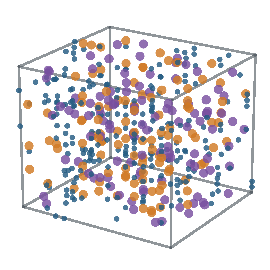
\includegraphics[width=2.45cm]{sampling_material_a_overview.pdf}};
 \node[font=\scriptsize,text=black!65] at (1.32,15.98)
   {strain samples $\{\ee^s\}$};
 \draw[flow] (2.56,17.95)--(3.02,17.95);
 \node[font=\tiny,text=black!60] at (2.79,18.20) {FOM};
 \node[inner sep=0pt] at (4.52,17.95)
   {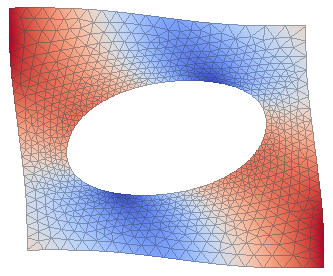
\includegraphics[width=3.05cm]{rve_deformed_overview.pdf}};
 \node[font=\scriptsize] at (4.52,15.98)
   {$\F^{s}\mapsto\bigl(W^{s},\ssv^{s}\bigr)$};

 \node[panel,minimum width=9.65cm,minimum height=5.00cm,anchor=south west,
       fill=orange!1] (featurepanel) at (6.45,15.50) {};
 \node[stage] at (6.81,20.12) {2};
 \node[font=\small\bfseries,anchor=west] at (7.19,20.12)
   {Learnable paired directional features};

 % Each sensor is explicitly drawn on the undeformed discretized RVE.
 \foreach \yy/\lab/\ang in {19.18/{z_1}/24,17.84/{z_2}/-12,16.25/{z_m}/48} {
   \node[inner sep=0pt] at (7.72,\yy)
     {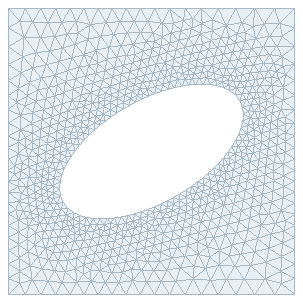
\includegraphics[width=.96cm]{rve_reference_overview.pdf}};
   \node[font=\scriptsize,anchor=east] at (7.17,\yy) {$\lab$};
   \coordinate (sensor) at (7.72,\yy);
   \draw[orange!85!black,line width=.85pt,-{Latex[length=1.1mm]}]
     (sensor)--++(\ang:.31);
   \draw[teal!75!black,line width=.85pt,-{Latex[length=1.1mm]}]
     (sensor)--++({\ang+90}:.31);
   \fill (sensor) circle (.85pt);
 }
 \node[font=\normalsize] at (7.72,17.04) {$\vdots$};

 \node[align=center,font=\small] at (11.90,17.68)
   {$\displaystyle z_i(\F,J)
     =\frac{\|\F\bm d_i\|^{2p_i}}{p_iJ^{b_i}}
     +\frac{\|\F\bm d_i^\perp\|^{2q_i}}{q_iJ^{c_i}}$};
 \node[align=center,font=\scriptsize,text=black!62] at (11.90,16.55)
   {orientation and exponents adapt to the RVE response\\
    within the analytic convexity bounds};
 \draw[orange!85!black,line width=.9pt,-{Latex[length=1.2mm]}]
   (11.30,19.12)--++(.55,0);
 \node[font=\scriptsize,anchor=west] at (11.99,19.12) {$\bm d_i$};
 \draw[teal!75!black,line width=.9pt,-{Latex[length=1.2mm]}]
   (11.30,18.62)--++(.55,0);
 \node[font=\scriptsize,anchor=west] at (11.99,18.62) {$\bm d_i^\perp$};

 \draw[flow] (rvepanel.east)--(featurepanel.west);

 \begin{scope}[yshift=.05cm]
 % -------------------------------------------------------------------------
 % Second level: a small, horizontal version of the core-architecture figure.
 % Information flows from left to right; ellipses stand for intervening layers.
 \node[panel,minimum width=16.10cm,minimum height=3.60cm,anchor=south west]
   (corepanel) at (0,11.40) {};
 \node[stage] at (.36,14.62) {3};
 \node[font=\small\bfseries,anchor=west] at (.74,14.62)
   {Monotone convex core};
 \draw[black!18] (8.05,11.60)--(8.05,14.35);
 \draw[flow] (featurepanel.south) -- (11.28,15.00);
 \node[font=\scriptsize,text=black!65,anchor=west] at (11.42,15.225)
   {conditioned input $\bm y(\bm z)$};

 % ICNN: learned nonnegative weights feed fixed softplus nodes.
 \node[font=\scriptsize\bfseries,text=icnncolor!80!black] at (4.03,14.10) {ICNN};
 \node[font=\scriptsize,text=black!65] at (4.03,13.76)
   {learned nonnegative weights, fixed softplus on nodes};
 \foreach \lx in {2.88,4.58}
   \filldraw[black!45,fill=black!3,line width=.6pt,rounded corners=1pt]
     (\lx-.33,11.92) rectangle (\lx+.33,13.40);
 \node[dot] (icin1) at (1.68,13.14) {};
 \node[dot] (icinm) at (1.68,12.18) {};
 \node[font=\scriptsize,anchor=east] at (1.56,13.14) {$y_1$};
 \node[font=\scriptsize,anchor=east] at (1.56,12.18) {$y_m$};
 \node[font=\scriptsize] at (1.68,12.72) {$\vdots$};
 \node[dot] (icout) at (5.78,12.66) {};
 \foreach \ya in {13.14,12.66,12.18} {
   \draw[weight] (icin1)--(2.644,\ya);
   \draw[weight] (icinm)--(2.644,\ya);
   \draw[weight] (4.816,\ya)--(icout);
   \foreach \yb in {13.14,12.66,12.18}
     \draw[weight] (3.116,\ya)--(4.344,\yb);
 }
 \fill[white] (3.53,11.95) rectangle (3.93,13.37);
 \foreach \ya in {13.14,12.66,12.18}
   \node[font=\scriptsize] at (3.73,\ya) {$\cdots$};
 \foreach \lx in {2.88,4.58}
   \foreach \ya in {13.14,12.66,12.18}
     \pic[scale=.62] at (\lx,\ya) {softplus};
 \node[font=\scriptsize,anchor=west] at (5.90,12.66) {$\widehat H(\bm y)$};
 % The conditioned input also enters the last hidden layer and the output.
 \draw[inputmap,rounded corners=2pt,-{Latex[length=1.1mm]}]
   (icinm)--(1.68,11.62)--(5.78,11.62)--(icout);
 \draw[inputmap,-{Latex[length=1mm]}] (4.58,11.62)--(4.58,11.90);

 % ICKAN: every edge carries its own learned convex, nondecreasing function.
 \node[font=\scriptsize\bfseries,text=ickancolor] at (12.08,14.10) {ICKAN};
 \node[font=\scriptsize,text=black!65] at (12.08,13.76)
   {learned convex, nondecreasing functions on edges};
 \filldraw[ickancolor,fill=ickancolor!4,line width=.6pt,rounded corners=1pt]
   (10.28,11.80) rectangle (10.72,13.52);
 \filldraw[ickancolor,fill=ickancolor!4,line width=.6pt,rounded corners=1pt]
   (12.76,11.98) rectangle (13.24,13.34);
 \node[dot] (kin1) at (9.80,13.14) {};
 \node[dot] (kinm) at (9.80,12.18) {};
 \node[font=\scriptsize,anchor=east] at (9.68,13.14) {$y_1$};
 \node[font=\scriptsize,anchor=east] at (9.68,12.18) {$y_m$};
 \node[font=\scriptsize] at (9.80,12.72) {$\vdots$};
 \foreach \j/\yn in {1/13.14,2/12.66,3/12.18} {
   \node[dot] (kfirst\j) at (11.30,\yn) {};
   \node[dot] (klast\j) at (12.35,\yn) {};
 }
 \node[dot] (kout) at (13.70,12.66) {};
 \foreach \j/\ya/\yb in {1/13.36/13.08,2/12.80/12.52,3/12.24/11.96} {
   \draw[connection] (kin1)--(10.50,\ya)--(kfirst\j);
   \draw[connection] (kinm)--(10.50,\yb)--(kfirst\j);
 }
 \foreach \j/\yn in {1/13.14,2/12.66,3/12.18} {
   \foreach \k in {1,2,3}
     \draw[connection] (kfirst\j)--(klast\k);
   \draw[connection] (klast\j)--(13.00,\yn)--(kout);
 }
 \fill[white] (11.63,11.95) rectangle (12.03,13.37);
 \foreach \yn in {13.14,12.66,12.18}
   \node[font=\scriptsize] at (11.83,\yn) {$\cdots$};
 \foreach \yy/\cc in {13.36/.70,13.08/.55,12.80/.80,12.52/.60,12.24/.75,11.96/.50}
   \pic[scale=.40] at (10.50,\yy) {edgecurve=\cc};
 \foreach \yy/\cc in {13.14/.72,12.66/.58,12.18/.66}
   \pic[scale=.45] at (13.00,\yy) {edgecurve=\cc};
 \node[font=\scriptsize,anchor=west] at (13.82,12.66) {$\widehat H(\bm y)$};
 % As in the deployed ICKAN, the conditioned input also has an output map.
 \draw[inputmap,rounded corners=2pt,-{Latex[length=1.1mm]}]
   (kinm)--(9.80,11.62)--(13.70,11.62)--(kout);
 \end{scope}
 \end{scope}

 % Both alternatives produce the same learned scalar contribution.
 \node[panel,minimum width=3.70cm,minimum height=.82cm]
   (hcore) at (8.05,5.89) {};
 \node[font=\scriptsize,align=center] at (8.05,5.98)
   {$H(\bm z)=\widehat H\!\left(\bm y(\bm z)\right)$};
 \node[font=\scriptsize,text=black!60] at (8.05,5.71)
   {learned contribution};
 \draw[secondaryflow] (corepanel.south)--(hcore.north);

 % -------------------------------------------------------------------------
 % Third level: analytic completion is part of the complete energy itself.
 \node[panel,minimum width=11.05cm,minimum height=3.60cm,
       anchor=south west] (energy) at (0,1.28) {};
 \node[stage] at (.36,4.49) {4};
 \node[font=\small\bfseries,anchor=west] at (1.08,4.49)
   {Complete stored energy};

 \node[font=\small,align=left] at (5.53,2.98)
   {$\displaystyle W(\F)=
      \underbrace{H(\bm z)-H(\bm z^0)}_{W_{\rm learn}}
      \underbrace{-r(J-1)}_{W_{\rm corr}}$\\[5pt]
    $\displaystyle \qquad+
      \underbrace{\alpha(J-1-\log J)+\frac{\beta}{2}(J-1)^2}_{W_{\rm vol}}
      +\underbrace{\varepsilon\!\left(\frac{\operatorname{tr}\C}{2}-1-\log J\right)}_{W_{\rm dist}}$};
 \node[font=\scriptsize,text=black!60] at (5.53,1.56)
   {reference state: $W(\I)=0,\qquad \ssv(\bm0)=\bm0$};

 \node[panel,minimum width=4.60cm,minimum height=3.60cm,
       anchor=south west] (response) at (11.50,1.28) {};
 \node[stage] at (11.87,4.49) {5};
 \node[font=\small\bfseries,anchor=west] at (12.25,4.49)
   {Constitutive output};
 \node[font=\small] at (13.80,3.38)
   {$\underbrace{\ssv=\nabla_{\ee}W}_{\text{stress}}$};
 \node[font=\small] at (13.80,2.05)
   {$\underbrace{\bm D=\nabla_{\ee}^{2}W}_{\text{tangent}}$};

 \draw[secondaryflow,rounded corners=2pt]
   (hcore.south) -- ++(0,-.22) -| (energy.north);
 \draw[flow] (energy.east)--(response.west);

 % Guarantee ribbon.  The six equally spaced entries reproduce criteria
 % (C1)--(C6) exactly; their labels replace manually positioned separators.
 \node[panel,fill=black!3,minimum width=16.10cm,minimum height=1.12cm]
   at (8.05,.60) {};
 \node[font=\footnotesize\bfseries] at (8.05,.96)
   {Criteria satisfied by construction};
 \node[font=\scriptsize,align=center,text=black!75]
   at (1.43,.43) {\textbf{(C1)} potential\\structure};
 \node[font=\scriptsize,align=center,text=black!75]
   at (4.08,.43) {\textbf{(C2)}\\objectivity};
 \node[font=\scriptsize,align=center,text=black!75]
   at (6.73,.43) {\textbf{(C3)} stress symmetry\\and anisotropy};
 \node[font=\scriptsize,align=center,text=black!75]
   at (9.38,.43) {\textbf{(C4)} reference\\normalization};
 \node[font=\scriptsize,align=center,text=black!75]
   at (12.03,.43) {\textbf{(C5)} 2D\\polyconvexity};
 \node[font=\scriptsize,align=center,text=black!75]
   at (14.68,.43) {\textbf{(C6)}\\growth};
\end{tikzpicture}

 \caption{Overview of the proposed constitutive construction. Sampled strain states are evaluated with the periodic RVE model to supply energy and stress data. These responses train learnable paired directional features and a monotone convex ICNN or ICKAN core. Analytic reference and growth terms complete the stored energy. Differentiation then supplies the work-conjugate stress and constitutive tangent. Criteria (C1)--(C6), defined in Section~\ref{sec:requirements}, follow from the complete construction rather than from sampled numerical checks.}
 \label{fig:constitutive_pipeline}
\end{figure}

Potential structure (C1), supplied by Eq.~\eqref{eq:energy_stress_relation}, implies that the work around every closed strain path $\Gamma$ satisfies
\begin{equation}
 \oint_{\Gamma}\ssv\cdot\dd\ee=0 .
 \label{eq:conservative_requirement}
\end{equation}
For the isothermal purely elastic setting considered here, (C1) likewise gives $\ssv\cdot\dot{\ee}-\dot W=0$, so the mechanical dissipation vanishes. The stress Jacobian is then the Hessian of $W$ and obeys the cross-derivative identities $\partial s_i/\partial e_j=\partial s_j/\partial e_i$, that is, the major symmetry $\bm D=\bm D^T$ of the constitutive tangent in Eq.~\eqref{eq:tangent}.

Objectivity (C2) must remove dependence on the spatial observer without inadvertently imposing material isotropy. For a superposed proper rotation $\bm Q$, it requires
\begin{equation}
 W(\bm Q\F)=W(\F),\qquad
 \bm P(\bm Q\F)=\bm Q\bm P(\F).
\end{equation}
Using $\C=\F^T\F$ as an energy input enforces the first identity, because a superposed spatial rotation leaves $\C$ unchanged. Differentiating the objective energy then gives the stress transformation. The stress symmetry required by (C3), $\Sg=\Sg^T$, follows for the energy models considered here from differentiation with respect to symmetric strain. It implies a symmetric Cauchy stress $\bm\sigma=J^{-1}\F\Sg\F^T$, as required by angular-momentum balance in the present continuum.

Objectivity still permits anisotropy, because material symmetry is a different invariance. A right action $\F\mapsto\F\bm Q_m$ leaves the energy unchanged precisely when $\bm Q_m$ belongs to the material symmetry group. Section~\ref{sec:feature_order} implements this distinction with directions attached to the reference material. A superposed spatial rotation acts on $\F$ from the left and does not alter the directional stretch measured in that reference. The major symmetry of $\bm D$ is a third, separate property, which follows from (C1) rather than from the symmetry of the stress tensor.

Reference normalization (C4) makes the learned energy consistent with the undeformed state by requiring
\begin{equation}
 W(\I)=0,\qquad \ssv(\bm0)=\bm0,
\end{equation}
where $\ssv(\bm0)=\bm0$ is equivalent to $\bm P(\I)=\bm0$. The first condition fixes an arbitrary additive energy constant. The second is a substantive stress condition, and the admissible correction depends on the model class. For the Unconstrained energy, Section~\ref{sec:tiers} subtracts the raw reference value and a term linear in $\E$. That correction preserves its scalar potential, but an arbitrary linear function of $\E$ need not preserve polyconvexity in $\F$. The ICNN and ICKAN energies instead use a correction that is affine in the determinant, which preserves convexity in the independent minors (Section~\ref{sec:energy_admissibility}).

Polyconvexity (C5) supplies the curvature control that potential structure leaves open. Direct convexity in $\F$ is generally too restrictive for objective finite-strain energies with singular-volume growth, so convexity is imposed instead in independent deformation minors~\cite{ball1977,Ciarlet1988}. In two dimensions,\footnote{The standard three-dimensional definition uses $(\F,\cof\F,\det\F)$. The two-dimensional guarantee established here does not imply an admissible extension to arbitrary out-of-plane deformation.} this means that the energy admits the representation
\begin{equation}
 W(\F)=\mathcal P(\F,\det\F),\qquad
 \mathcal P\text{ convex in its independent arguments}.
 \label{eq:polyconvex_definition}
\end{equation}
Here $\mathcal P$ is defined on the convex set $\R^{2\times2}\times(0,\infty)$, treating its matrix and scalar arguments as independent. Only its evaluation in $W$ sets the second argument equal to $\det\F$. The cofactor is linear in the entries of a $2\times2$ matrix, so it need not be introduced as an additional independent argument. Convexity of $\mathcal P$ implies that $W$ cannot curve downward along an admissible rank-one perturbation of $\F$.

Convexity in $\C$ or $\E$, as imposed in strain-space formulations such as that of As'ad et al.~\cite{asad2022}, does not imply polyconvexity~\cite{GaoNeffRoventaThiel2017}, because $\E=\tfrac12(\F^T\F-\I)$ depends quadratically on $\F$. Appendix~\ref{app:finite_strain_curvature} derives the rank-one consequence of (C5), states its differential form, and gives an analytical counterexample for convexity in $\E$.

Growth (C6) guards against volume collapse and unbounded deformation, which a polyconvex energy may still allow. It requires $W\to\infty$ as $J\to0^+$, as $J\to\infty$, and as $\|\F\|\to\infty$ while $J$ remains bounded away from zero and infinity. These conditions contribute to coercivity. Existence of a minimizer also requires admissible boundary data and finite-energy competitors~\cite{Ciarlet1988}, and no constitutive barrier guarantees convergence of a full Newton iteration.

\subsection{Unconstrained energy reference}
\label{sec:tiers}
The Unconstrained energy is a smooth neural network $\widehat W_{\theta}$ acting on
\begin{equation}
 \bm x(\ee)=\big(C_{11}-1,C_{22}-1,C_{12},J-1\big)^T.
 \label{eq:unconstrained_inputs}
\end{equation}
Here $\C=\I+2\E$ and $J=\sqrt{\det\C}$, so the four inputs are functions of the same three engineering-strain components. Using components of $\C$ in a material reference basis ensures objectivity under superposed spatial rotations but does not impose isotropy, since the network may depend differently on $C_{11}$, $C_{22}$, and $C_{12}$. Denote the resulting raw energy by $\widetilde W(\ee)=\widehat W_{\theta}(\bm x(\ee))$. A generic network does not satisfy the reference conditions automatically, so the normalized energy is defined, following the consistency correction of As'ad et al.~\cite{asad2022}, as
\begin{equation}
 W_{\mathrm{unc}}(\ee)=\widetilde W(\ee)-\widetilde W(\bm0)
 -\partial_{\ee}\widetilde W(\bm0)\cdot\ee.
 \label{eq:unconstrained_energy}
\end{equation}
By construction, $W_{\mathrm{unc}}(\bm0)=0$ and $\partial_{\ee}W_{\mathrm{unc}}(\bm0)=\bm0$. Because the correction is affine in $\ee$, it leaves the Hessian of the raw network unchanged, so the reference energy and stress are fixed while the learned curvature remains unrestricted.

\subsection{Feature design: expressiveness and admissibility}
\label{sec:feature_order}
The first design question is how to describe deformation without erasing the effective anisotropy of the RVE. Classical invariants provide the natural starting point. In two dimensions, the principal invariants of $\C$ are $I_1=\tr\C$ and $\det\C=J^2$, and they determine all three invariants of the plane-strain embedding $\diag(\C,1)$. They describe principal stretches without recording their orientation relative to the material, so an energy depending only on them is isotropic.

To retain directional information, one can supplement the isotropic measures with a structural direction $\bm d$. The familiar anisotropic stretch invariant is
\begin{equation}
 I_4(\bm d)=\bm d^T\C\bm d
          =\C:(\bm d\otimes\bm d)=\|\F\bm d\|^2,
 \qquad \|\bm d\|=1.
 \label{eq:directional_invariant}
\end{equation}
It measures squared stretch along a material direction and remains unchanged by a superposed spatial rotation. Such directional invariants are standard ingredients of anisotropic hyperelastic energies~\cite{SchroderNeff2003,Gasser2006}. Here $\bm d$ need not represent a physical fiber. Learned directions serve as objective scalar descriptors of the RVE's effective anisotropy. In two dimensions, $\bm d$ is naturally accompanied by its perpendicular $\bm d^\perp$. For this orthonormal pair,
\begin{equation}
 I_4(\bm d)+I_4(\bm d^\perp)=I_1,\qquad
 \|\cof\F\,\bm d\|^2=I_4(\bm d^\perp).
 \label{eq:directional_invariant_2d}
\end{equation}
The first identity shows that the pair splits $I_1$ between two perpendicular directions, so that its two members retain the directional information that $I_1$ discards. The second shows that a cofactor-based directional measure reads the stretch in the perpendicular direction rather than introducing an independent third in-plane descriptor.

Objective directional descriptors solve only the first part of the design problem. Because the learned contribution $H(\bm z)$ is nondecreasing in each feature, the feature vector $\bm z(\F)$ also determines which deformation states it must order. For any two deformation states,
\begin{equation}
 \bm z(\F_B)\geq\bm z(\F_A)\text{ componentwise}
 \quad\Longrightarrow\quad H(\bm z(\F_B))\geq H(\bm z(\F_A)),
 \label{eq:feature_ordering}
\end{equation}
whatever the width of the network. As anticipated in Section~\ref{sec:discussion}, this ordering constrains the learned contribution but not the analytic normalization and growth terms, so the feature map must be designed together with them. Additional features remain functions of the same three engineering-strain components and introduce no new strain variable, but they embed the strain state into more variables on which the core is monotone and convex. They can enlarge the admissible response family without guaranteeing that it contains the target response.

The paired construction below is designed to retain directional stretch, reshape the componentwise ordering seen by the monotone core, and remain convex in the independent variables $(\F,J)$. It meets these three objectives by coupling directional stretch to volume through admissible determinant exponents. A feature can consequently decrease along a path when its denominator grows sufficiently, even if a numerator increases. Its reference derivative is also controlled analytically, which will allow the reference stress to be removed without sacrificing convexity.

\subsubsection{Paired directional features}
Let $m$ denote the number of scalar features. For each $i=1,\ldots,m$, let $\bm d_i=(\cos\theta_i,\sin\theta_i)^T$ and $\bm d_i^\perp=(-\sin\theta_i,\cos\theta_i)^T$. Define
\begin{equation}
 \begin{aligned}
 z_i(\F,J)
 &=\frac{I_4(\bm d_i)^{p_i}}{p_i J^{b_i}}
          +\frac{I_4(\bm d_i^\perp)^{q_i}}{q_i J^{c_i}}\\
 &=\frac{\|\F\bm d_i\|^{2p_i}}{p_i J^{b_i}}
          +\frac{\|\F\bm d_i^\perp\|^{2q_i}}{q_i J^{c_i}},
 \end{aligned}
 \label{eq:features}
\end{equation}
where $\theta_i$ sets the orientation of the reference directions, $p_i,q_i$ are the powers of the squared-stretch invariants, and $b_i,c_i$ control each contribution's coupling to the area ratio $J$. These roles provide expressiveness, but the exponents cannot be chosen arbitrarily if the feature is to remain convex. They satisfy
\begin{equation}
 p_i,q_i\geq\tfrac12,\qquad
 0\leq b_i\leq2p_i-1,\qquad 0\leq c_i\leq2q_i-1.
 \label{eq:featureconstraints}
\end{equation}
The lower bounds on $p_i$ and $q_i$ make the corresponding powers of the directional norms convex, while the upper bounds on $b_i$ and $c_i$ prevent their coupling with $J$ from introducing a negative-curvature direction. Appendix~\ref{app:convex} derives these conditions from the Hessian of a single stretch--determinant contribution.
In the learned-feature variants, $\theta_i$ and the four exponent parameters are optimized, with $p_i,q_i,b_i,c_i$ subject to Eq.~\eqref{eq:featureconstraints}. The fixed-feature controls of Section~\ref{sec:constitutive_training} hold the same initialized feature parameters constant while training the core. With unconstrained parameters $\widehat p_i,\widehat q_i,\widehat b_i,\widehat c_i\in\R$ and the functions $\operatorname{softplus}(x)=\log(1+e^x)$ and $\operatorname{sigmoid}(x)=(1+e^{-x})^{-1}$, whose ranges are $(0,\infty)$ and $(0,1)$, the exponents are
\begin{equation}
 \begin{aligned}
 p_i&=\tfrac12+\operatorname{softplus}(\widehat p_i),
 &b_i&=(2p_i-1)\operatorname{sigmoid}(\widehat b_i),\\
 q_i&=\tfrac12+\operatorname{softplus}(\widehat q_i),
 &c_i&=(2q_i-1)\operatorname{sigmoid}(\widehat c_i).
 \end{aligned}
 \label{eq:feature_parameterization}
\end{equation}
The angles require no admissibility bound, because the maps $\F\mapsto\F\bm d_i$ and $\F\mapsto\F\bm d_i^\perp$ remain linear in $\F$ for any fixed $\theta_i$. Equation~\eqref{eq:feature_parameterization} satisfies the bounds of Eq.~\eqref{eq:featureconstraints} strictly for all finite parameter values, approaching the boundary only as a limit, so no penalty is needed during training. Each $z_i$ is one scalar feature with two perpendicular contributions. Because their exponents need not be equal, the pairing does not impose invariance under their interchange.

The construction was also designed to simplify reference normalization. Its paired and scaled contributions make the reference strain gradient of every feature isotropic. Consequently, the learned contribution has an isotropic reference stress, which a single scalar determinant correction can cancel in Section~\ref{sec:energy_admissibility}. The following result gathers the objectivity, convexity, and reference-state properties needed there.

\begin{proposition}
\label{prop:paired_features}
Under the constraints in Eq.~\eqref{eq:featureconstraints}, each feature in Eq.~\eqref{eq:features} is objective and convex in the independent variables $(\F,J)$ on $J>0$. Its value and engineering-strain gradient at the identity, evaluated with $J=\det\F$, are
\begin{equation}
 z_i^0=\frac1{p_i}+\frac1{q_i},\qquad
 \partial_{\ee}z_i\big|_{\bm0}=\rho_i(1,1,0)^T,
 \qquad \rho_i=2-\frac{b_i}{p_i}-\frac{c_i}{q_i}.
 \label{eq:referencefeatures}
\end{equation}
\end{proposition}
The proof is given in Appendix~\ref{app:convex}. The mechanism behind the reference gradient is that $1/p_i$ and $1/q_i$ cancel the stretch-power multipliers upon differentiation. The two perpendicular directional contributions then sum to $2\I$, while the determinant terms contribute $-(b_i/p_i+c_i/q_i)\I$. Hence $\rho_i$ is the amplitude of an isotropic reference gradient, with equal normal components and zero shear. This reference property does not imply isotropy of the response away from the reference state.

The raw features are now mechanically admissible, but their numerical magnitudes may differ. Before the features enter the core, they are centered and scaled as $y_i=(z_i-z_i^{\rm cen})/\tau_i$, with a centering value $z_i^{\rm cen}$ and a scale $\tau_i>0$ that are independent of deformation for any fixed parameter set. This positive affine conditioning preserves both convexity in independent $(\F,J)$ and the componentwise ordering required by the monotone core. The choices used in the constitutive assessments are specified in Section~\ref{sec:training_protocol}.

\subsection{Monotone ICNN and integrated-hat ICKAN cores}
\label{sec:convex_cores}
Section~\ref{sec:feature_order} supplies features $z_i$ that are objective and convex in the independent variables $(\F,J)$. The remaining question is how a learned core may combine them, through the conditioned vector $\bm y=(y_1,\ldots,y_m)^T$, without undoing that convexity.

Composition with the convex feature map preserves convexity only when the core is convex and componentwise nondecreasing~\cite{klein2022,linden2023}. The two cores enforce these properties differently. The ICNN learns nonnegative linear maps and applies fixed softplus activations at its hidden nodes, whereas the ICKAN learns a convex, nondecreasing scalar function on every edge and sums the incoming contributions at each node (Fig.~\ref{fig:convex_core_architectures}).

\begin{figure}[tbp]
 \centering% General multilayer schematic of the deployed monotone core families.
% Ellipses denote repeated hidden layers; widths and curves are illustrative.
% Purple paths bundle nonnegative linear maps of the entire original input.
% Model colours match the data figures: ICNN green, ICKAN blue; fixed
% operators are neutral.
\definecolor{icnncolor}{HTML}{2AA780}%
\definecolor{ickancolor}{HTML}{2B5DAA}%
\begin{tikzpicture}[x=1cm,y=1cm,font=\small,
  weight/.style={draw=icnncolor!90!black,line width=.75pt},
  connection/.style={draw=black!60,line width=.6pt},
  inputmap/.style={draw=violet!65!black,dashed,line width=.65pt},
  maparrow/.style={inputmap,-{Latex[length=1.4mm]}},
  dot/.style={circle,fill=black,inner sep=0pt,minimum size=4pt},
  callout/.style={-{Latex[length=1.8mm]},draw=black,line width=.75pt},
  annotation/.style={font=\small\itshape,align=center,text width=3.15cm,inner sep=2pt},
  pics/softplus/.style={code={
    \draw[draw=black!55,fill=white,line width=.45pt]
      (-.44,-.32) rectangle (.44,.32);
    \draw[black!25,line width=.2pt]
      (-.33,-.22) -- (.34,-.22) (-.33,-.22) -- (-.33,.24);
    \draw[black!70,line width=.7pt]
      plot[domain=-3:3,samples=35]
      ({.11*\x},{-.22+.42*(ln(1+exp(\x))-ln(1+exp(-3)))/3});
  }},
  pics/hatcurve/.style args={#1/#2}{code={
    \draw[draw=ickancolor,fill=white,line width=.4pt]
      (-.44,-.32) rectangle (.44,.32);
    \draw[black!25,line width=.2pt]
      (-.33,-.22) -- (.34,-.22) (-.33,-.22) -- (-.33,.24);
    \draw[ickancolor!85!black,line width=.6pt]
      plot[domain=-1.5:1.5,samples=41]
      ({.22*\x},{-.22+.42*(#1*(\x+1.5)
        +#2*(max(\x+1,0)^3-2*max(\x,0)^3+max(\x-1,0)^3)/6)
        /(3*#1+1.5*#2)});
  }}
]
 \path[use as bounding box] (0,.45) rectangle (16.2,9.45);
 \fill[icnncolor!7] (1.6,8.75) rectangle (8.9,9.45);
 \fill[ickancolor!7] (8.9,8.75) rectangle (16.2,9.45);
 \fill[black!2] (0,1.1) rectangle (1.6,9.45);
 \draw[black!65,line width=.5pt] (0,.45) rectangle (16.2,9.45);
 \foreach \tablex in {1.6,8.9}
   \draw[black!65,line width=.5pt] (\tablex,1.1) -- (\tablex,9.45);
 \foreach \tabley in {1.1,7.2,8.75}
   \draw[black!65,line width=.5pt] (0,\tabley) -- (16.2,\tabley);
 \node[font=\small\bfseries] at (.8,9.1) {Core};
 \node[font=\small\bfseries] at (5.25,9.1) {Monotone ICNN};
 \node[font=\small\bfseries] at (12.55,9.1) {Monotone integrated-hat ICKAN};
 \node[align=center,font=\footnotesize] at (.8,7.98) {Layer\\operation};
 \node[align=center,font=\footnotesize] at (.8,4.15) {Multilayer\\core};
 \node[align=center,text width=6.6cm] at (5.25,7.98)
   {\textcolor{icnncolor!80!black}{Learned nonnegative linear weights} + biases\\[3pt]
    $\longrightarrow$ \textcolor{black!70}{fixed softplus at hidden nodes}};
 \node[align=center,text width=6.6cm] at (12.55,7.98)
   {\textcolor{ickancolor}{One learned scalar function per edge}\\[2pt]
    \textcolor{ickancolor}{(convex and nondecreasing)}\\[2pt]
    $\longrightarrow$ sum at nodes + biases};

 % ICNN: information flows from the conditioned input at the top to the
 % scalar output at the bottom, consistently with the paper overview.
 \begin{scope}[xshift=1.6cm,yshift=1.35cm]
  \node[anchor=west,font=\small\bfseries] at (.12,5.55) {(a)};
  \node[font=\footnotesize,text=violet!65!black] (icinputvector) at (1.6,5.62)
    {input $\bm y$};
  \foreach \level in {4.05,1.70}
    \filldraw[black!45,fill=black!3,line width=.75pt]
      (.02,\level-.25) rectangle (3.18,\level+.25);
  \node[dot] (icinput1) at (.9,5.10) {};
  \node[dot] (icinputm) at (2.3,5.10) {};
  \node[font=\footnotesize] at (.9,5.34) {$y_1$};
  \node[font=\footnotesize] at (2.3,5.34) {$y_m$};
  \node[font=\footnotesize] at (1.6,5.10) {$\cdots$};
  \node[dot] (icoutput) at (1.6,.55) {};
  \node[font=\footnotesize] at (1.6,.12) {$\widehat H(\bm y)$};
  \foreach \j in {0,...,2} {
    \pgfmathsetmacro{\hiddenx}{.35+1.25*\j}
    \draw[weight] (icinput1) -- (\hiddenx,4.05);
    \draw[weight] (icinputm) -- (\hiddenx,4.05);
    \draw[weight] (\hiddenx,1.70) -- (icoutput);
    \foreach \k in {0,...,2} {
      \pgfmathsetmacro{\nextx}{.35+1.25*\k}
      \draw[weight] (\hiddenx,4.05) -- (\nextx,1.70);
    }
  }
  \fill[white] (.02,2.70) rectangle (3.23,3.13);
  \foreach \hiddenx in {.35,1.6,2.85}
    \node at (\hiddenx,2.91) {$\vdots$};

  % Direct input map to the output, and bundled maps into later preactivations.
  \draw[inputmap,rounded corners=2pt] (icinputvector.east)
    -- (3.7,5.62) -- (3.7,.55);
  \draw[maparrow] (3.7,.55) -- (icoutput.east);
  \draw[inputmap] (3.7,2.22) -- (.35,2.22);
  \foreach \hiddenx in {.35,1.6,2.85}
    \draw[maparrow] (\hiddenx,2.22) -- (\hiddenx,1.95);
  \node[fill=white,inner sep=1pt,text=violet!65!black] at (3.7,2.91) {$\vdots$};
  \foreach \j in {0,...,2} {
    \pgfmathsetmacro{\hiddenx}{.35+1.25*\j}
    \pic[scale=.58] at (\hiddenx,4.05) {softplus};
    \pic[scale=.58] at (\hiddenx,1.70) {softplus};
  }
  \node[annotation,text=black!70] (icfixed) at (5.65,4.15)
    {Nonlinear, fixed\\softplus activations};
  \node[annotation,text=icnncolor!80!black] (icweights) at (5.65,3.05)
    {Learned nonnegative\\linear weights};
  \node[annotation,text=violet!65!black] (icmaps) at (5.65,1.25)
    {Original input to later\\hidden layers and output};
  \draw[callout] (3.21,4.05) to[out=0,in=195] (icfixed.west);
  \draw[callout] (3.16,3.18) to[out=0,in=180] (icweights.west);
  \draw[callout] (3.77,1.25) -- (icmaps.west);
 \end{scope}

 % ICKAN: the same top-to-bottom convention; every displayed edge contains
 % its own learned scalar function before the receiving sum node.
 \begin{scope}[xshift=8.9cm,yshift=1.35cm]
  \node[anchor=west,font=\small\bfseries] at (.12,5.55) {(b)};
  \node[font=\footnotesize,text=violet!65!black] (kaninputvector) at (1.6,5.62)
    {input $\bm y$};
  \foreach \level in {4.55,2.25,1.05}
    \filldraw[ickancolor,fill=ickancolor!4,line width=.75pt]
      (0,\level-.22) rectangle (3.26,\level+.22);
  \node[dot] (kaninput1) at (.9,5.10) {};
  \node[dot] (kaninputm) at (2.3,5.10) {};
  \node[font=\footnotesize] at (.9,5.34) {$y_1$};
  \node[font=\footnotesize] at (2.3,5.34) {$y_m$};
  \node[font=\footnotesize] at (1.6,5.10) {$\cdots$};
  \node[dot] (kanoutput) at (1.6,.55) {};
  \node[font=\footnotesize] at (1.6,.12) {$\widehat H(\bm y)$};
  \foreach \j in {0,...,2} {
    \pgfmathsetmacro{\hiddenx}{.35+1.25*\j}
    \node[dot] (kanfirst\j) at (\hiddenx,3.95) {};
    \node[dot] (kanlast\j) at (\hiddenx,1.70) {};
  }
  \foreach \j in {0,...,2} {
    \pgfmathsetmacro{\hiddenx}{.35+1.25*\j}
    \draw[connection] (kanlast\j) -- (\hiddenx,1.05) -- (kanoutput);
    \foreach \r in {0,1} {
      \pgfmathsetmacro{\edgex}{.27+.53*(2*\j+\r)}
      \ifnum\r=0
        \draw[connection] (kaninput1) -- (\edgex,4.55) -- (kanfirst\j);
      \else
        \draw[connection] (kaninputm) -- (\edgex,4.55) -- (kanfirst\j);
      \fi
    }
    \foreach \k in {0,...,2} {
      \pgfmathsetmacro{\edgex}{.16+.36*(3*\j+\k)}
      \draw[connection] (kanfirst\k) -- (\edgex,2.25) -- (kanlast\j);
    }
  }
  \fill[white] (.02,2.78) rectangle (3.27,3.20);
  \foreach \hiddenx in {.35,1.6,2.85}
    \node at (\hiddenx,2.99) {$\vdots$};
  \foreach \j in {0,...,2} {
    \pgfmathsetmacro{\hiddenx}{.35+1.25*\j}
    \pgfmathsetmacro{\slope}{.08+.25*\j}
    \pgfmathsetmacro{\curvature}{1.5-.45*\j}
    \pic[scale=.45] at (\hiddenx,1.05) {hatcurve=\slope/\curvature};
    \foreach \r in {0,1} {
      \pgfmathsetmacro{\edgex}{.27+.53*(2*\j+\r)}
      \pgfmathsetmacro{\slope}{.08+.15*\j+.2*\r}
      \pgfmathsetmacro{\curvature}{1.4-.3*\j-.2*\r}
      \pic[scale=.39] at (\edgex,4.55) {hatcurve=\slope/\curvature};
    }
    \foreach \k in {0,...,2} {
      \pgfmathsetmacro{\edgex}{.16+.36*(3*\j+\k)}
      \pgfmathsetmacro{\slope}{.08+.11*\j+.14*\k}
      \pgfmathsetmacro{\curvature}{1.5-.23*\j-.25*\k}
      \pic[scale=.30] at (\edgex,2.25) {hatcurve=\slope/\curvature};
    }
  }
  \draw[inputmap,rounded corners=2pt] (kaninputvector.east)
    -- (3.7,5.62) -- (3.7,.55);
  \draw[maparrow] (3.7,.55) -- (kanoutput.east);
  \node[annotation,text=ickancolor] (kanfunctions) at (5.65,4.42)
    {One learned convex,\\nondecreasing function\\per edge};
  \node[annotation] (kansums) at (5.65,3.13) {Sum operation\\at nodes};
  \node[annotation,text=violet!65!black] (kanmap) at (5.65,1.25)
    {Linear map from\\input to output};
  \draw[callout] (3.29,4.55) to[out=0,in=170] (kanfunctions.west);
  \draw[callout] (3.0,3.95) to[out=0,in=130] (kansums.west);
  \draw[callout] (3.77,1.25) -- (kanmap.west);
 \end{scope}

 % Colour legend of the operators.
 \draw[weight,line width=1pt] (.35,.78) -- (.85,.78);
 \node[anchor=west,font=\footnotesize] at (.98,.78) {Learned linear weights};
 \pic[scale=.40] at (5.05,.78) {softplus};
 \node[anchor=west,font=\footnotesize] at (5.42,.78) {Fixed softplus};
 \pic[scale=.40] at (9.05,.78) {hatcurve=.1/1.3};
 \node[anchor=west,font=\footnotesize] at (9.42,.78) {Learned spline functions};
 \draw[inputmap,line width=1pt] (13.35,.78) -- (13.85,.78);
 \node[anchor=west,font=\footnotesize] at (13.98,.78) {Input maps};
\end{tikzpicture}

 \caption{Multilayer monotone cores mapping the conditioned paired features $\bm y$ to the scalar contribution $\widehat H(\bm y)$. (a) The ICNN learns nonnegative linear maps and applies fixed softplus activations at hidden nodes. (b) The ICKAN learns one convex, nondecreasing scalar function per edge and sums them at nodes. Purple dashed paths denote nonnegative maps of the complete input, and ellipses denote intervening layers. Glyph counts indicate where each operation acts, not deployed widths or parameter counts. Unrestricted biases are omitted.}
 \label{fig:convex_core_architectures}
\end{figure}

\subsubsection{Monotone ICNN}
\label{sec:icnn_core}
Let $L$ denote the number of hidden layers and $\bm a^{(\ell)}$ the vector of activations in layer $\ell$, for $\ell=1,\ldots,L$. Here $\widehat H(\bm y)$ denotes the scalar neural core acting on the conditioned features $\bm y$, to which the complete energy of Section~\ref{sec:energy_admissibility} adds the reference-normalization and growth terms. The deployed ICNN has the form
\begin{align}
 \bm a^{(1)}&=\phi(\bm U_1\bm y+\bm b_1),\nonumber\\
 \bm a^{(\ell)}&=\phi(\bm W_\ell\bm a^{(\ell-1)}+\bm U_\ell\bm y+\bm b_\ell),
 \qquad \ell=2,\ldots,L,\nonumber\\
 \widehat H(\bm y)&=\bm v^T\bm a^{(L)}+\bm w^T\bm y+b_{\rm out},
 \label{eq:monotone_icnn}
\end{align}
where $\phi=\operatorname{softplus}$ is applied componentwise. Its derivatives satisfy $\phi'(x)=\operatorname{sigmoid}(x)>0$ and $\phi''(x)=\operatorname{sigmoid}(x)[1-\operatorname{sigmoid}(x)]>0$. The activation is smooth, increasing, and convex, and its smoothness makes the core $C^2$, as required for a continuous constitutive tangent. The matrices $\bm U_\ell$ and $\bm W_\ell$ contain the weights from $\bm y$ and the preceding hidden layer, respectively, and $\bm b_\ell$ is the layer bias vector. The output weight vectors $\bm v$ and $\bm w$ act on $\bm a^{(L)}$ and $\bm y$, respectively, and $b_{\rm out}$ is an additive scalar output bias.

Every entry of $\bm W_\ell,\bm U_\ell,\bm v,\bm w$ is nonnegative, enforced by softplus transformations of unconstrained weight parameters. These signs play two related but distinct roles. The matrices $\bm W_\ell$ and the output vector $\bm v$ multiply convex hidden activations, so their nonnegativity preserves convexity as well as monotonicity. The maps $\bm U_\ell\bm y$ and $\bm w^T\bm y$ are affine, so they leave convexity unchanged for either sign, but nonnegative $\bm U_\ell$ and $\bm w$ are required for componentwise monotonicity. Biases are unrestricted because adding constants to a preactivation preserves both properties. Hidden biases can change the core's derivatives with respect to $\bm y$, whereas $b_{\rm out}$ only shifts $\widehat H$ and leaves its derivatives unchanged.

The preservation argument proceeds layer by layer. The first hidden layer is convex because softplus is convex and its argument is affine, and it is nondecreasing because $\bm U_1$ is nonnegative. Assuming that $\bm a^{(\ell-1)}$ is convex and nondecreasing, the nonnegative map $\bm W_\ell\bm a^{(\ell-1)}$, the nonnegative affine input map, and composition with $\phi$ preserve both properties in layer $\ell$. The same argument applies to the output, proving by induction that $\widehat H$ is convex and componentwise nondecreasing. This is the ICNN composition argument of Amos et al.~\cite{amos2017}, supplemented here by nonnegative direct-input maps to guarantee monotonicity.

\subsubsection{Monotone integrated-hat ICKAN}
\label{sec:ickan_core}
With $\bm h^{(0)}=\bm y$ and $n_\ell$ the width of layer $\ell$, where $n_0=m$, the hidden layers and scalar output of the ICKAN are
\begin{align}
 h_j^{(\ell)}
 &=\sum_{i=1}^{n_{\ell-1}}f_{ji}^{(\ell)}\!\left(h_i^{(\ell-1)}\right)
   +b_j^{(\ell)},
 &&j=1,\ldots,n_\ell,\quad \ell=1,\ldots,L,\nonumber\\
 \widehat H(\bm y)
 &=\sum_{i=1}^{n_L}f_i^{\rm out}\!\left(h_i^{(L)}\right)
   +\bm w^T\bm y+b_{\rm out},
 &&\bm w\geq\bm0.
 \label{eq:monotone_ickan}
\end{align}
Here $f_{ji}^{(\ell)}$ transforms the scalar carried by one edge and $h_j^{(\ell)}$ is the sum formed at a node. The nonnegative linear skip $\bm w^T\bm y$ connects the conditioned input directly to the scalar output.
\begin{samepage}
It remains to specify the functions appearing on the edges. For any $f_{ji}^{(\ell)}$ or $f_i^{\rm out}$ in Eq.~\eqref{eq:monotone_ickan}, let $x$ denote its scalar input. Each edge uses the common form
\begin{equation}
 f(x)=a x+\sum_k c_k B_k(x),\qquad a,c_k\geq0,
 \label{eq:splineedge}
\end{equation}
where $a$ is the learned linear slope, $c_k$ are learned weights of the spline bases $B_k$, and $k$ indexes these bases. Softplus transformations of unconstrained parameters impose the signs of $a$ and $c_k$. Additive constants are represented once, through the unrestricted node biases in Eq.~\eqref{eq:monotone_ickan}, rather than redundantly on every incoming edge.
\end{samepage}

To exclude negative slope and curvature by construction, the curvature of each edge is parameterized directly. Each $B_k''$ is a nonnegative triangular hat centered at a knot $\kappa_k$. The knots form a fixed uniform grid with spacing $h>0$ that is not optimized. Writing $s=(x-\kappa_k)/h$, one curvature basis is
\begin{equation}
 B_k''(x)=\max(1-|s|,0).
 \label{eq:hat_curvature}
\end{equation}
Integrating twice from the left conditions $B_k(x)=B_k'(x)=0$ for $x\leq\kappa_k-h$ gives
\begin{equation}
 B_k(x)=h^2\begin{cases}
 0,&s\leq-1,\\
 (s+1)^3/6,&-1<s\leq0,\\
 (-s^3+3s^2+3s+1)/6,&0<s<1,\\
 s,&s\geq1.
 \end{cases}
 \label{eq:hat}
\end{equation}
Figure~\ref{fig:integrated_hat_construction} shows both levels of the construction: integration of one curvature basis and assembly of a learned edge from several bases.
\begin{figure}[tbp]
 \centering% Analytic schematic of one integrated-hat basis and a learned edge assembled
% from several nonnegative curvature contributions.  Curves in panel (a) are
% exact for kappa=0 and h=1; panel (b) is a qualitative multi-basis schematic.
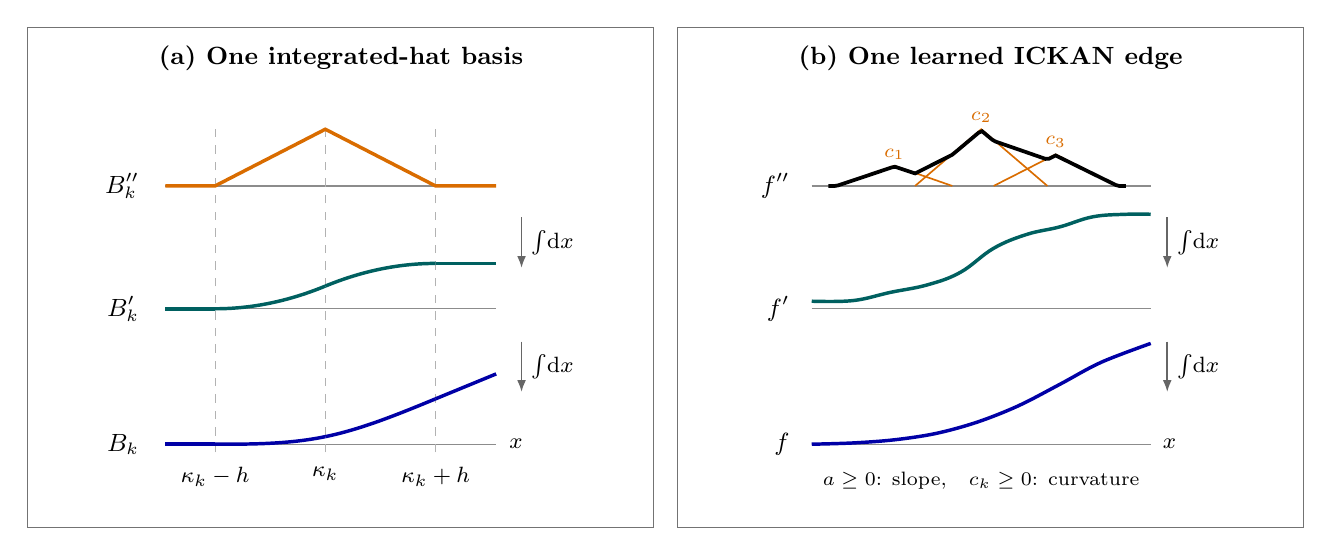
\begin{tikzpicture}[x=1cm,y=1cm,font=\small,
  axis/.style={draw=black!45,line width=.45pt},
  guide/.style={draw=black!30,dashed,line width=.4pt},
  curvature/.style={draw=orange!85!black,line width=1.25pt},
  slope/.style={draw=teal!75!black,line width=1.25pt},
  basis/.style={draw=blue!65!black,line width=1.25pt},
  total/.style={draw=black,line width=1.35pt},
  integrate/.style={-{Latex[length=1.5mm]},draw=black!60,line width=.55pt}
]
 \path[use as bounding box] (0,0) rectangle (16.2,6.35);
 \draw[black!55,line width=.5pt] (0,0) rectangle (7.95,6.35);
 \draw[black!55,line width=.5pt] (8.25,0) rectangle (16.2,6.35);

 \node[font=\small\bfseries] at (3.98,5.96) {(a) One integrated-hat basis};
 \node[font=\small\bfseries] at (12.23,5.96) {(b) One learned ICKAN edge};

 % Panel (a): exact normalized single-basis construction.  The larger left
 % inset keeps all row labels inside the panel.
 \begin{scope}[xshift=3.78cm,yshift=.62cm,x=1.40cm,y=.80cm]
  \foreach \yy/\lab in {4.65/{$B_k''$},2.70/{$B_k'$},.55/{$B_k$}} {
    \draw[axis] (-1.45,\yy) -- (1.55,\yy);
    \node[anchor=east] at (-1.60,\yy) {\lab};
  }
  \foreach \xx in {-1,0,1}
    \draw[guide] (\xx,.42) -- (\xx,5.55);

  \draw[curvature] (-1.45,4.65) -- (-1,4.65) -- (0,5.55)
    -- (1,4.65) -- (1.55,4.65);

  \draw[slope] (-1.45,2.70) -- (-1,2.70);
  \draw[slope] plot[domain=-1:0,samples=35]
    (\x,{2.70+.72*(\x+1)^2/2});
  \draw[slope] plot[domain=0:1,samples=35]
    (\x,{2.70+.72*(.5+\x-.5*\x^2)});
  \draw[slope] (1,3.42) -- (1.55,3.42);

  \draw[basis] (-1.45,.55) -- (-1,.55);
  \draw[basis] plot[domain=-1:0,samples=35]
    (\x,{.55+.72*(\x+1)^3/6});
  \draw[basis] plot[domain=0:1,samples=35]
    (\x,{.55+.72*(-\x^3+3*\x^2+3*\x+1)/6});
  \draw[basis] plot[domain=1:1.55,samples=15]
    (\x,{.55+.72*\x});

  \draw[integrate] (1.78,4.15) -- node[right,font=\footnotesize] {$\int\!\dd x$} (1.78,3.35);
  \draw[integrate] (1.78,2.18) -- node[right,font=\footnotesize] {$\int\!\dd x$} (1.78,1.38);
  \node[font=\footnotesize,anchor=north] at (-1,.34) {$\kappa_k-h$};
  \node[font=\footnotesize,anchor=north] at (0,.34) {$\kappa_k$};
  \node[font=\footnotesize,anchor=north] at (1,.34) {$\kappa_k+h$};
  \node[font=\footnotesize,anchor=west] at (1.58,.55) {$x$};
 \end{scope}

 % Panel (b): nonnegative learned combination of several fixed hats.
 \begin{scope}[xshift=12.11cm,yshift=.62cm,x=1.05cm,y=.80cm]
  \foreach \yy/\lab in {4.65/{$f''$},2.70/{$f'$},.55/{$f$}} {
    \draw[axis] (-2.05,\yy) -- (2.05,\yy);
    \node[anchor=east] at (-2.20,\yy) {\lab};
  }

  % Individual learned curvature contributions, in the curvature colour of
  % panel (a); their sum is drawn in black.
  \draw[orange!85!black,line width=.6pt]
    (-1.75,4.65) -- (-1.05,4.97) -- (-.35,4.65);
  \draw[orange!85!black,line width=.6pt]
    (-.80,4.65) -- (0,5.55) -- (.80,4.65);
  \draw[orange!85!black,line width=.6pt]
    (.15,4.65) -- (.90,5.15) -- (1.65,4.65);
  \draw[total] plot[domain=-1.85:1.75,samples=90]
    (\x,{4.65+.88*(.35*max(1-abs((\x+1.05)/.7),0)
      +max(1-abs(\x/.8),0)+.55*max(1-abs((\x-.9)/.75),0))});
  \node[font=\scriptsize,text=orange!85!black] at (-1.05,5.15) {$c_1$};
  \node[font=\scriptsize,text=orange!85!black] at (0,5.74) {$c_2$};
  \node[font=\scriptsize,text=orange!85!black] at (.90,5.35) {$c_3$};

  % Monotone accumulated slope and convex connection (schematic).
  \draw[slope] plot[smooth,tension=.65] coordinates {
    (-2.05,2.82) (-1.55,2.83) (-1.10,2.96) (-.65,3.08)
    (-.25,3.28) (.15,3.66) (.55,3.88) (.95,4.00)
    (1.35,4.16) (1.75,4.20) (2.05,4.20)};
  \draw[basis] plot[smooth,tension=.55] coordinates {
    (-2.05,.55) (-1.55,.57) (-1.05,.62) (-.55,.72)
    (-.05,.90) (.45,1.16) (.95,1.50) (1.45,1.85)
    (2.05,2.15)};

  \draw[integrate] (2.25,4.15) -- node[right,font=\footnotesize] {$\int\!\dd x$} (2.25,3.35);
  \draw[integrate] (2.25,2.18) -- node[right,font=\footnotesize] {$\int\!\dd x$} (2.25,1.38);
  \node[font=\footnotesize,anchor=west] at (2.08,.55) {$x$};
  \node[font=\scriptsize,align=center] at (0,-.03)
    {$a\geq0$: slope,\quad $c_k\geq0$: curvature};
 \end{scope}
\end{tikzpicture}

 \caption{Integrated-hat parameterization of an ICKAN edge. (a) A localized nonnegative curvature hat integrates to a nonnegative slope and a convex $C^2$ basis with a zero left tail and a linear right tail. (b) Nonnegative learned coefficients combine several fixed bases into a nonnegative edge curvature, and integration gives a nondecreasing slope and a convex, nondecreasing connection. The curves illustrate the analytic construction, not the deployed grid.}
 \label{fig:integrated_hat_construction}
\end{figure}

The value and first two derivatives in Eq.~\eqref{eq:hat} match at every join, and $B_k''$ vanishes at the outer joins, so $B_k$ is globally $C^2$. Its curvature is localized to $[\kappa_k-h,\kappa_k+h]$, whereas the integrated basis has a zero left tail and a linear right tail. Moreover, $B_k'(-\infty)=0$ and $B_k''\geq0$ imply $B_k'\geq0$. The complete edge therefore satisfies
\begin{equation}
 f''(x)=\sum_k c_kB_k''(x)\geq0,
 \qquad
 f'(x)=a+\sum_k c_kB_k'(x)\geq0,
 \label{eq:splineedge_guarantees}
\end{equation}
for every learned parameter set with $a,c_k\geq0$, which makes each edge convex and nondecreasing by construction.

Because every edge is convex and nondecreasing, induction across the layers of Eq.~\eqref{eq:monotone_ickan} shows that every $h_j^{(\ell)}$, and finally $\widehat H$, is convex and componentwise nondecreasing in $\bm y$. The nonnegative input-to-output skip preserves both properties. The fixed knot grid and finite number of bases limit where an individual edge can learn curvature, since outside their combined support the edge has linear tails. These tails are linear in the scalar input $x$ only, and the complete energy remains nonlinear in $\F$ through the features and the analytic growth terms. The grid used in the constitutive assessment is reported in Section~\ref{sec:training_protocol}. This core is inspired by the monotonic input-convex KAN framework~\cite{thakolkaran2025}, with the integrated-hat bases and analytic tails specified here.

\subsection{The complete energy and its admissibility guarantees}
\label{sec:energy_admissibility}
Sections~\ref{sec:feature_order} and~\ref{sec:convex_cores} constructed the physical feature vector $\bm z$, its conditioned representation $\bm y(\bm z)$, and the scalar neural core $\widehat H(\bm y)$, which together define the learned contribution
\begin{equation}
 H(\bm z)=\widehat H\bigl(\bm y(\bm z)\bigr).
 \label{eq:conditioned_neural_contribution}
\end{equation}
This term represents the anisotropic response. The energy and stress references and the growth toward the boundary of the admissible deformation domain are set by analytic terms.

The residual stress produced by $H$ at the undeformed state is quantified first. With $\bm z^0=\bm z(\I,1)$ and the feature-gradient factors $\rho_i$ of Eq.~\eqref{eq:referencefeatures}, the core sensitivities and the scalar amplitude of this residual stress are
\begin{equation}
 h_i=\partial_{z_i}H(\bm z^0)\geq0,
 \qquad
 r=\sum_i h_i\rho_i.
\end{equation}
For a fixed parameter set, $H(\bm z^0)$ and $r$ are constants with respect to deformation. The complete stored energy then combines the learned contribution with analytic reference-normalization and growth terms,
\begin{align}
 W(\F)={}&\underbrace{H(\bm z)-H(\bm z^0)}_{\text{(i) }W_{\rm learn}}
 +\underbrace{\big[-r(J-1)\big]}_{\text{(ii) }W_{\rm corr}}\nonumber\\
 &+\underbrace{\alpha(J-1-\log J)+\frac\beta2(J-1)^2}_{\text{(iii) }W_{\rm vol}}\nonumber\\
 &+\underbrace{\varepsilon\left(\frac{\tr\C}{2}-1-\log J\right)}_{\text{(iv) }W_{\rm dist}},
 \qquad \alpha,\beta,\varepsilon>0.
 \label{eq:energy}
\end{align}
Here $J=\det\F$, $\C=\F^T\F$, and $\bm z=\bm z(\F,J)$. The positive energy-density coefficients $\alpha$, $\beta$, and $\varepsilon$ weight the analytic growth terms. For either core, the composition in Eq.~\eqref{eq:conditioned_neural_contribution} is twice continuously differentiable, convex, and componentwise nondecreasing in $\bm z$.

Each of the four contributions named by the underbraces solves a distinct constitutive problem:
\begin{itemize}
 \item[(i)] The term $W_{\rm learn}$ carries the learned response and fixes the energy reference. At $\F=\I$, the features equal $\bm z^0$, and hence
 \begin{equation}
  W(\I)=H(\bm z^0)-H(\bm z^0)=0.
  \label{eq:energy_reference_value}
 \end{equation}
 The remaining terms also vanish because $J=1$ and $\tr\C=2$. Since $H(\bm z^0)$ is constant with respect to deformation, its subtraction fixes the energy reference without changing the stress or tangent.

 \item[(ii)] The correction $W_{\rm corr}$ removes the reference stress, which a constant subtraction cannot change. By the chain rule and Eq.~\eqref{eq:referencefeatures}, the learned contribution has the reference value
 \begin{equation}
  \left.\nabla_{\ee}H(\bm z)\right|_0
  =\sum_i h_i\left.\nabla_{\ee}z_i\right|_0
  =\sum_i h_i\rho_i(1,1,0)^T
  =r(1,1,0)^T.
  \label{eq:neural_reference_stress}
 \end{equation}
 The identity $J=\sqrt{(1+2E_{11})(1+2E_{22})-(2E_{12})^2}$ gives $\nabla_{\ee}J|_0=(1,1,0)^T$. Holding $r$ fixed when differentiating yields
 \begin{equation}
  \left.\nabla_{\ee}\big[H(\bm z)-r(J-1)\big]\right|_0
  =r(1,1,0)^T-r(1,1,0)^T=\bm0.
  \label{eq:energy_reference_stress}
 \end{equation}
 A single scalar $r$ suffices because the paired features make the reference stress isotropic (Proposition~\ref{prop:paired_features}). The correction is zero in value at $J=1$ and, being affine in the independent determinant variable, preserves convexity for either sign of $r$. Linden et al.~\cite{linden2023} use the same affine determinant term to normalize isotropic energies but need additional invariant terms for anisotropic ones, whereas Eq.~\eqref{eq:referencefeatures} makes the isotropic form sufficient for the paired features.

 \item[(iii)] The volumetric term $W_{\rm vol}$ controls growth in $J$. Its logarithmic part diverges as $J\to0^+$, where the quadratic part alone would remain finite with limit $\beta/2$. The quadratic part dominates the linear correction $-r(J-1)$ as $J\to\infty$, so the energy diverges under expansion for either sign of $r$. At the reference,
 \begin{equation}
  W_{\rm vol}(1)=0,\qquad
  W_{\rm vol}'(J)=\alpha(1-J^{-1})+\beta(J-1),\qquad
  W_{\rm vol}'(1)=0,
 \end{equation}
 so this term leaves the reference energy and stress unchanged.

 \item[(iv)] The distortional term $W_{\rm dist}$ supplies growth under area-preserving changes of shape, which a function of $J$ alone cannot detect. For example, with $\lambda>0$,
 \begin{equation}
  \F=\diag(\lambda,\lambda^{-1}),\qquad
  J=1,\qquad
  \varepsilon\left(\frac{\tr\C}{2}-1-\log J\right)
  =\frac\varepsilon2\left(\lambda^2+\lambda^{-2}-2\right).
 \end{equation}
 This contribution diverges as $\lambda\to\infty$, although the area remains constant. More generally, $\tr\C=\|\F\|_F^2$ supplies growth under unbounded deformation at bounded positive $J$. At the reference, the constant $-1$ sets its value to zero. Using $\C=\I+2\E$ and $\partial_{\E}J|_0=\I$, its stress contribution is
 \begin{equation}
  \left.\partial_{\E}\left[\varepsilon\left(\frac{\tr\C}{2}-1-\log J\right)\right]\right|_0
  =\varepsilon\left[\I-\left.J^{-1}\partial_{\E}J\right|_0\right]
  =\bm0.
 \end{equation}
\end{itemize}
Together, $W_{\rm learn}$ and $W_{\rm corr}$ set the learned response and its reference state, while $W_{\rm vol}$ and $W_{\rm dist}$ prescribe growth toward the boundary of the admissible domain. Although the analytic terms vanish with their first derivatives at the reference, they still contribute to the reference stiffness, because $J$ is nonlinear in $\ee$. The following proposition gathers the guarantees of their complete sum.

\begin{proposition}
\label{prop:complete_energy}
Let the features satisfy Eq.~\eqref{eq:featureconstraints}, let the core be either of the $C^2$ convex, componentwise nondecreasing constructions in Section~\ref{sec:convex_cores}, and let $\alpha,\beta,\varepsilon>0$. Then Eq.~\eqref{eq:energy} defines a $C^2$, objective, two-dimensional polyconvex energy on $\GL$. Its associated second Piola--Kirchhoff stress $\Sg$ is symmetric, its work-conjugate representation is $\ssv=\nabla_{\ee}W$, $W(\I)=0$, $\ssv(\bm0)=\bm0$, and $W$ diverges under collapse, unbounded expansion, and unbounded distortion at bounded positive area. Thus the construction satisfies (C1)--(C6).
\end{proposition}
The proof is given in Appendix~\ref{app:complete_energy_proof}. In brief, the convex, componentwise nondecreasing core preserves feature convexity, the remaining terms are constant, affine, or convex in independent $(\F,J)$, and the reference identities and growth limits complete the argument.

The three constitutive constructions carried into the numerical assessment are summarized in Table~\ref{tab:tiers}. The ICNN and ICKAN columns include both fixed- and learned-feature variants, and learning the feature parameters changes the representation while leaving the guarantees above intact.
\begin{table}[htbp]
\centering\small
\caption{Constitutive constructions carried into the numerical assessment. Criteria (C1)--(C6) are defined in Section~\ref{sec:requirements}, and the guarantees refer to the constructions of this section.}
\label{tab:tiers}
\begin{tabularx}{\linewidth}{lYYY}
\toprule
 & \shortstack{Unconstrained\\energy} & ICNN & ICKAN\\
\midrule
Role & Flexible hyperelastic reference & Guaranteed paired-feature energy & Guaranteed paired-feature energy\\
\midrule
Inputs & Objective measures from $(\C,J)$ & \shortstack{Paired features\\(fixed or learned)} & \shortstack{Paired features\\(fixed or learned)}\\
\midrule
Learned scalar map & Smooth energy network & \shortstack{Nonnegative weights;\\fixed activations} & \shortstack{Convex, nondecreasing\\edge functions}\\
\midrule
(C1)--(C4) & By construction & By construction & By construction\\
\midrule
(C5)--(C6) & Not imposed & By construction & By construction\\
\bottomrule
\end{tabularx}
\end{table}
\FloatBarrier

\section{Projection-based reduced-order models}
\label{sec:reduced}
The periodic RVE problem of Section~\ref{sec:fom} has $N$ independent displacement coordinates, and the nested FOM--FE$^2$ calculation solves it at every macroscopic integration point and Newton iteration. Its solutions, however, depend on only three strain components, so the microscopic states visited by a structural calculation form a three-parameter family. Projection-based model order reduction exploits this structure by collecting FOM solutions as snapshots and seeking each new state in a space learned from them.

These snapshots are taken of the independent state $\bm u\in\R^N$, obtained from the physical nodal displacement vector $\bm d\in\R^{N_{\rm dof}}$ after enforcing periodicity and removing rigid translation. In the deployed convention,
\begin{equation}
 \bm d(\bm u,\ee)=\bm T\bm u+\bm g_{\rm per}(\ee),
 \qquad \bm R(\bm u;\ee)=\bm T^T\bm f_{\rm int}
                 \bigl(\bm d(\bm u,\ee)\bigr)=\bm0.
 \label{eq:hdm_lifting}
\end{equation}
Here $\bm T$ identifies periodic degrees of freedom, and the lifting $\bm g_{\rm per}$ supplies the strain-dependent displacement jumps and anchor values of Section~\ref{sec:fom}, so any independent state $\bm u$ produces a physical field that satisfies the prescribed kinematic constraints. With $\bm K_{\rm phys}=\partial_{\bm d}\bm f_{\rm int}$ the assembled physical stiffness, the FOM tangent is $\bm K=\partial_{\bm u}\bm R=\bm T^T\bm K_{\rm phys}\bm T$, and all residuals follow the internal-force sign convention.

Because $\bm u=\bm a+\bm u_{\rm aff}(\ee)$ adds to the fluctuation coordinates $\bm a$ of Eq.~\eqref{eq:microeq} the affine displacement $\bm u_{\rm aff}$ at the independent nodes, the snapshots retain the affine part of the displacement. This choice leaves the periodic boundary conditions unchanged and keeps the load-correlated information used by the strain-informed identification below, so the reported POD dimension characterizes this representation and its truncation tolerance.

\subsection{POD approximation and the affine PROM}
FOM solutions $\bm u^s$ at sampled strains $\ee^s$, $s=1,\ldots,N_s$, are centered about a reference state $\bm u_{\rm ref}$, and the singular value decomposition (SVD) of the snapshot matrix
\begin{equation}
 \bm S_{\rm snap}=
 [\,\bm u^1-\bm u_{\rm ref},\ldots,\bm u^{N_s}-\bm u_{\rm ref}\,]
 =\bm U_S\bm\Sigma_S\bm Y_S^T.
 \label{eq:snapshot_svd}
\end{equation}
supplies the POD modes. The $n_{\rm tra}$ leading left singular vectors form the orthonormal reduced-order basis (ROB) $\bm V_{\rm tra}$ of the affine approximation
\begin{equation}
 \widetilde{\bm u}=\bm u_{\rm ref}+\bm V_{\rm tra}\qq_{\rm tra},
 \qquad \qq_{\rm tra}\in\R^{n_{\rm tra}},
 \qquad \bm V_{\rm tra}^T\bm V_{\rm tra}=\bm I.
 \label{eq:linear_prom}
\end{equation}
which replaces the $N$ independent displacement coordinates by $n_{\rm tra}\ll N$ modal amplitudes. The subscript ``tra'' marks this traditional affine approximation, and the term affine refers only to the approximation space, since the constitutive law and the reduced equilibrium equations remain nonlinear.

The retained dimension is selected from the relative squared reconstruction error, which for a Euclidean POD is
\begin{equation}
 \epsilon_{\rm POD}^2(n_{\rm tra})=
 \frac{\sum_{j>n_{\rm tra}}\sigma_j^2}{\sum_j\sigma_j^2}.
 \label{eq:pod_tail}
\end{equation}
This criterion measures how well the snapshots are compressed but does not bound the stress error at unsampled strains, because force evaluation, constitutive differentiation, and equilibrium conditioning can make small displacement components important.

Galerkin projection onto the admissible variations $\delta\widetilde{\bm u}=\bm V_{\rm tra}\delta\qq_{\rm tra}$ gives the reduced equations and tangent at a prescribed strain $\ee$,
\begin{equation}
 \bm r_{\rm tra}(\qq_{\rm tra};\ee)
 =\bm V_{\rm tra}^T
  \bm R(\bm u_{\rm ref}+\bm V_{\rm tra}\qq_{\rm tra};\ee)=\bm0,
 \quad
 \bm K_{\rm tra}=\bm V_{\rm tra}^T\bm K\bm V_{\rm tra}.
 \label{eq:linear_galerkin}
\end{equation}
The system now has $n_{\rm tra}$ unknowns, but evaluating $\bm R$ and $\bm K$ still visits every microscopic element, which the hyperreduction of Section~\ref{sec:hyperreduction} addresses.

\subsection{Nonlinear reduction through latent-space closure}
\label{sec:latent_closure}
The POD dimension required to reconstruct a displacement field can exceed the number of coordinates needed to parametrize the loading family. Latent-space closure exploits this distinction by retaining a rich linear span while learning dependencies among its modal amplitudes, so that only a smaller subset remains unknown in equilibrium~\cite{barnett2023,aresdeparga2026nonlinear}. Because the leading POD coefficients need not provide a well-conditioned primary-to-secondary map, the input-informed construction of Hern\'andez et al.~\cite{hernandez2026dimensional} instead combines the retained modal amplitudes linearly into $n=3$ primary coordinates $\bm\xi$, approximately aligned with the three macroscopic strain components. It splits the retained $n_{\rm tot}$-dimensional span into orthonormal primary and secondary blocks $\bm V\in\R^{N\times n}$ and $\overline{\bm V}\in\R^{N\times\bar n}$, with $n_{\rm tot}=n+\bar n$, and an ANN closure $\widehat{\mathcal N}:\R^n\to\R^{\bar n}$ predicts the secondary coordinates $\overline{\qq}=\overline{\bm V}^T(\bm u-\bm u_{\rm ref})$. The deployed decoder and its tangent are
\begin{equation}
 \widetilde{\bm u}(\bm\xi)=\bm u_{\rm ref}
   +\bm V\bm A_m\bm\xi
   +\overline{\bm V}\widehat{\mathcal N}(\bm\xi),
 \qquad
 \bm B_\xi=\partial_{\bm\xi}\widetilde{\bm u},
 \label{eq:deployed_decoder}
\end{equation}
where $\bm A_m$ is the nonsingular coordinate transformation of the construction. The ANN predicts modal amplitudes of the microscopic displacement, not stress or energy, and the secondary modes remain in that field without appearing as independent equilibrium unknowns.

The closure is trained on the snapshot pairs $(\bm\xi^s,\overline{\qq}^{\,s})$ by minimizing
\begin{equation}
 \mathcal L_{\rm cl}(\bm\eta)=
 \frac{1}{|\mathcal I_{\rm fit}|\bar n}
 \sum_{s\in\mathcal I_{\rm fit}}
 \|\widehat{\mathcal N}(\bm\xi^s;\bm\eta)-\overline{\qq}^{\,s}\|_2^2.
 \label{eq:closure_loss}
\end{equation}
The closure must be smooth, because projection requires the derivatives of the decoder. This coordinate loss measures displacement reconstruction within the secondary space.

Because the alignment $\bm\xi^s\approx\ee^s$ is only fitted from the snapshots, the iterative PROM--ANN solves at fixed $\ee$ for the state satisfying
\begin{equation}
 \bm r(\bm\xi;\ee)=\bm B_\xi^T
       \bm R(\widetilde{\bm u}(\bm\xi);\ee)=\bm0,
 \label{eq:manifold_galerkin}
\end{equation}
rather than imposing $\bm\xi=\ee$. The exact Newton derivative then includes the curvature of the decoder manifold, since $\bm B_\xi$ depends on the state. Appendix~\ref{app:latent_closure} gives the coordinate construction, the reconstruction-error split, and this tangent explicitly.

\subsection{Hyperreduction of the projected equations}
\label{sec:hyperreduction}
Hyperreduction replaces each full element sum in the projected equations with a sparse weighted sum, a second approximation introduced after the displacement representation has been chosen. Two integration tasks must be distinguished: assembling the projected equilibrium equations and recovering the homogenized stress. Hernández et al.~\cite{hernandez2026dimensional} formulate both tasks and discuss the use of either a common or a dedicated stress rule. Separate elementwise rules are used here because the two integrands and their accuracy requirements differ.

\subsubsection{Fixed elementwise cubature}
Let $\mathcal E$ be the microscopic element set and $\bm L_e$ extract element nodal values from $\bm d$. At fixed macroscopic input, define the reconstructed element state and its reduced tangent by
\begin{equation}
 \bm d_e=\bm L_e(\bm T\widetilde{\bm u}+\bm g_{\rm per}),
 \qquad \bm B_e=\bm L_e\bm T\bm B .
\end{equation}
The full reduced residual is $\sum_{e\in\mathcal E}\bm h_e$, where
$\bm h_e=\bm B_e^T\bm f_{{\rm int},e}$. Fixed ECM approximates it as
\begin{equation}
 \bm r_{\rm ECM}(\qq;\ee)=
       \sum_{e\in\mathcal Z_r}w_e\bm h_e(\qq;\ee)=\bm0,
 \quad \mathcal Z_r\subset\mathcal E,\quad w_e\geq0.
 \label{eq:ecm}
\end{equation}
Here $\qq$ denotes the equilibrium unknowns and $\bm B=\partial_{\qq}\widetilde{\bm u}$ the decoder tangent, namely $\qq_{\rm tra}$ and $\bm V_{\rm tra}$ for the affine HPROM and $\bm\xi$ and $\bm B_\xi$ for HPROM--ANN. A selected element retains its ordinary within-element quadrature, so selected elements, selected Gauss points, and independent coordinates are distinct counts.

Offline, the element contributions are collected over $N_c$ training states and compressed by an SVD truncated, as in Eq.~\eqref{eq:pod_tail}, at a tolerance $\varepsilon_{\rm SVD}$. ECM then selects a sparse support and nonnegative multipliers that reproduce the retained integration modes~\cite{hernandez2017}. If $\bm G_{\rm cub}$ denotes those modes augmented by the constant-integration constraint (Appendix~\ref{app:cubature}) and $\bm b_{\rm cub}=\bm G_{\rm cub}\bm1$, selection stops when
\begin{equation}
 \frac{\|\bm G_{\rm cub}\bm w-\bm b_{\rm cub}\|_2}
      {\|\bm b_{\rm cub}\|_2}\leq\varepsilon_{\rm ECM}.
 \label{eq:ecm_tolerance}
\end{equation}
The residual rule integrates the element contributions $\bm h_e$, and the stress rule those to the average first Piola--Kirchhoff stress (Appendix~\ref{app:cubature}). Their supports and weights remain fixed online.

\subsubsection{Manifold-adaptive weights}
\label{sec:adaptive_weights}
A fixed rule must represent every sampled state with the same multipliers. MAW--ECM instead retains one common support but lets its weights vary over the reduced manifold~\cite{hernandez2026dimensional}. Applied to the residual, this gives
\begin{equation}
 \bm r_{\rm MAW}(\qq;\ee)=
 \sum_{e\in\mathcal Z_r}w_e(\qq)\bm B_e(\qq)^T
                   \bm f_{{\rm int},e}(\bm d_e)=\bm0.
 \label{eq:maw}
\end{equation}
Starting from a fixed ECM rule, the MAW--ECM pruning algorithm removes elements while redistributing nonnegative statewise weights, through the local and graph-regularized stages described by Hernández et al.~\cite{hernandez2026dimensional}. Pruning identifies the support but not the continuous online map, and neural fields are used here for that final regression stage. Because the equilibrium and stress rules are separate, two maps, $\mathcal N_r$ and $\mathcal N_s$, are trained on independently pruned supports $\mathcal Z_r$ and $\mathcal Z_s$,
\begin{equation}
 \begin{aligned}
  \bm w(\bm\xi)&=N_{\rm el}\operatorname{softmax}
                 \bigl(\mathcal N_r(\bm\xi;\bm\theta_r)\bigr),
   &\sum_{e\in\mathcal Z_r}w_e&=N_{\rm el},\\
  \bm v(\bm\xi)&=N_{\rm el}\operatorname{softmax}
                 \bigl(\mathcal N_s(\bm\xi;\bm\theta_s)\bigr),
   &\sum_{e\in\mathcal Z_s}v_e&=N_{\rm el}.
 \end{aligned}
 \label{eq:softmax_weights}
\end{equation}
The scaled softmax guarantees positivity and normalization. Unlike the closure, these networks predict integration weights, fitted against full-mesh element sums with the loss of Appendix~\ref{app:cubature}.

Online, the current reduced iterate is passed to both the closure and $\mathcal N_r$, and $\mathcal N_s$ supplies the stress weights, with the supports and all network parameters fixed. Differentiating the adaptive residual produces three contributions: element stiffness, decoder curvature, and weight variation. Only the first enters the microscopic modified-Newton iteration, which changes the convergence rate but not the converged state. For the affine HPROM, the decoder curvature and weight-variation terms vanish, so its projected stiffness is the exact residual Jacobian.

To translate sparse cubature into wall-clock savings, each optimized reduced mesh contains only the selected elements and the nodes they require. The corresponding basis operators and periodic lifting are restricted to that support before online evaluation. Online cost therefore depends on the support size, the retained secondary dimension, the equilibrium iterations, and the derivative evaluation, and not only on the number of primary coordinates.

\subsection{Constitutive output}
\label{sec:reduced_outputs}
Each HPROM must return the same work-conjugate stress and tangent required by the FE$^2$ problem. The stress rule reconstructs the average first Piola--Kirchhoff stress as
\begin{equation}
 \bm P_h(\qq,\ee)=
 \frac1{|Y|}\sum_{e\in\mathcal Z_s}v_e(\qq)
        \sum_{g\in e}\omega_g\bm P_{\mu,g}(\bm d_e),\qquad
 \Sg_h=\F^{-1}\bm P_h ,
 \label{eq:hyperreduced_stress}
\end{equation}
where $v_e$ is fixed for HPROM and state dependent for HPROM--ANN. Because this independently fitted rule need not give an exactly symmetric $\Sg_h$, its symmetric part supplies the returned components $\ssv_h(\qq,\ee)$.

Reduced equilibrium defines an implicit state $\qq^*(\ee)$ and hence the constitutive map $\ssv_h(\qq^*(\ee),\ee)$. If the residual Jacobian is nonsingular, differentiating equilibrium gives
\begin{equation}
 \bm D_h=\ssv_{h,\ee}
       -\ssv_{h,\qq}\bm r_{h,\qq}^{-1}\bm r_{h,\ee},
 \label{eq:reduced_ift}
\end{equation}
whose partial derivatives, evaluated at the converged state, include the decoder curvature and, for adaptive rules, the weight variation. This tangent, rather than the modified-Newton matrix of Section~\ref{sec:adaptive_weights}, is returned to the structural solver, and Appendix~\ref{app:cubature} records how its derivatives are evaluated.

When input-informed coordinates closely approximate the loading parameters, the decoder can also be evaluated without solving reduced equilibrium, as discussed by Hern\'andez et al.~\cite{hernandez2026dimensional} for their hyperelastic example. Prescribing $\bm\xi=\ee$ in Eq.~\eqref{eq:deployed_decoder} gives the direct decoder $\widetilde{\bm u}_{D}(\ee)=\widetilde{\bm u}(\bm\xi=\ee)$ of D-HPROM--ANN, whose state enters the same adaptive stress rule, with the same closure and stress weights, and whose tangent is the derivative of this direct stress map.

Figure~\ref{fig:reduced_model_hierarchy} traces the three resulting routes, from the offline RVE snapshots through the affine and nonlinear state representations to this common stress--tangent output.

\begin{figure}[p]
 \centering% Didactic overview of the intrusive reduced references.
% Rows 1--3 explain the offline state construction; rows 4--5 summarize the
% three online operating modes and their common constitutive interface.
% Colours encode roles only: green for FOM data and reconstructed states, blue
% for coordinates solved by equilibrium, red for the secondary part predicted
% by the ANN.  Model names and shared panels stay neutral, so that no colour
% repeats the ICNN/ICKAN/Unconstrained identities of the other figures.
\definecolor{hpromblue}{RGB}{0,105,210}%
\begin{tikzpicture}[x=1cm,y=1cm,font=\small,
  panel/.style={draw=black!55,rounded corners=2pt,line width=.55pt,fill=white},
  card/.style={draw=black!35,rounded corners=1.5pt,line width=.45pt,fill=white},
  flow/.style={-{Latex[length=2mm]},draw=black!70,line width=.8pt},
  flowline/.style={draw=black!70,line width=.8pt},
  secondaryflow/.style={-{Latex[length=1.7mm]},draw=black!55,line width=.65pt},
  stage/.style={circle,draw=black!60,fill=black!72,text=white,
                font=\bfseries\footnotesize,minimum size=5.2mm,inner sep=0pt},
  snapshot/.style={draw=green!45!black,fill=green!23,line width=.55pt},
  affineblock/.style={draw=hpromblue!85!black,fill=hpromblue!24,line width=.65pt},
  basisprimary/.style={draw=blue!65!black,fill=blue!14,line width=.55pt},
  basissecondary/.style={draw=red!55!black,fill=red!14,line width=.55pt},
  statevector/.style={draw=green!45!black,fill=green!17,line width=.55pt},
  coordprimary/.style={draw=blue!65!black,fill=blue!8,rounded corners=1pt},
  coordsecondary/.style={draw=red!55!black,fill=red!8,rounded corners=1pt},
  neuron/.style={circle,draw=black!45,fill=white,minimum size=2.4mm,inner sep=0pt}
]
 \path[use as bounding box] (0,0) rectangle (16.2,21.2);

 % -----------------------------------------------------------------------
 % Row 1: generate microscopic displacement snapshots.
 \node[panel,minimum width=16.10cm,minimum height=3.05cm,anchor=south west]
   (generation) at (0,18.02) {};
 \node[stage] at (.36,20.67) {1};
 \node[font=\small\bfseries,anchor=west] at (.74,20.67)
   {RVE snapshot generation};

 \node[inner sep=0pt] (sampling) at (1.42,19.32)
   {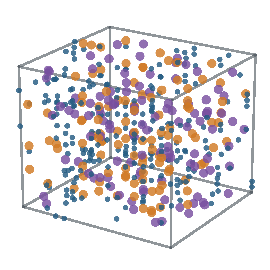
\includegraphics[width=1.58cm]{sampling_material_a_overview.pdf}};
 \node[font=\scriptsize,text=black!62] at (1.42,18.33)
   {sampled strains $\ee^s$};
 \node[inner sep=0pt] (rvesolve) at (4.30,19.32)
   {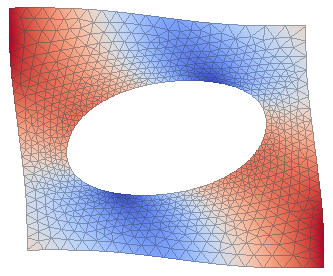
\includegraphics[width=2.10cm]{rve_deformed_overview.pdf}};
 \node[font=\scriptsize,align=center] at (4.30,18.33)
   {periodic FOM solve};
 \draw[flow] (sampling.east)--(rvesolve.west);
 \node[font=\tiny,text=black!58] at (2.73,19.57) {apply $\ee^s$};

 % Every column is a centered FOM state with the same dimension N.
 \node[font=\tiny,text=black!58] at (8.15,20.25)
   {$\widehat{\bm u}^{\,s}:=\bm u^s-\bm u_{\rm ref}$};
 \foreach \xx/\lab in {7.05/{\widehat{\bm u}^{\,1}},
                         7.92/{\widehat{\bm u}^{\,2}}} {
   \draw[snapshot] ({\xx-.21},18.64) rectangle ({\xx+.21},20.04);
   \node[font=\tiny] at (\xx,19.34) {$\lab$};
 }
\draw[snapshot] (9.29,18.64) rectangle (9.71,20.04);
\node[font=\tiny] at (9.50,19.34)
  {\scalebox{0.76}{$\scriptscriptstyle\widehat{\bm u}^{\,N_s}$}};
 \node[font=\normalsize] at (8.72,19.34) {$\cdots$};
 \node[font=\scriptsize,align=center] at (8.15,18.33)
   {centered displacement snapshots};
 \draw[flow] (rvesolve.east)--(6.72,19.32);

 \node[font=\scriptsize] at (13.30,20.25) {snapshot matrix};
 % Four vector-width units suggest the assembly of several N-vectors.
 \node[snapshot,minimum width=1.68cm,minimum height=1.40cm]
   (snapmatrix) at (13.30,19.34) {$\bm S_{\rm snap}$};
 \node[font=\tiny,text=black!58] at (13.30,18.46) {$N\times N_s$};
 \draw[flow] (9.84,19.32)--(snapmatrix.west);

 % -----------------------------------------------------------------------
 % Row 2: the same snapshot matrix generates either basis organization.
 \node[panel,minimum width=16.10cm,minimum height=3.10cm,anchor=south west,
       fill=black!1] (bases) at (0,14.60) {};
 \node[stage] at (.36,17.30) {2};
 \node[font=\small\bfseries,anchor=west] at (.74,17.30)
   {From the snapshot matrix to the reduced bases};

 % The matrix assembled in row 1 feeds both basis constructions directly.
 \node[card,minimum width=5.55cm,minimum height=2.02cm] (affinebasis)
   at (4.03,15.67) {};
 \node[font=\scriptsize] at (4.03,16.42) {affine basis};
 \draw[affineblock] (3.47,14.88) rectangle (4.59,16.28);
 \node[font=\scriptsize] at (4.03,15.58) {$\bm V_{\rm tra}$};
 \node[font=\tiny,text=black!58] at (4.03,14.75)
   {$N\times n_{\rm tra}$};

 \node[card,minimum width=5.55cm,minimum height=2.02cm] (splitbasis)
   at (12.08,15.67) {};
 \node[font=\scriptsize] at (12.08,16.42) {partitioned basis};
 \draw[basisprimary] (11.52,14.88) rectangle (11.94,16.28);
 \draw[basissecondary] (11.94,14.88) rectangle (12.64,16.28);
 \node[font=\scriptsize] at (11.73,15.58) {$\bm V$};
 \node[font=\scriptsize] at (12.29,15.58) {$\overline{\bm V}$};
 \node[font=\tiny,text=black!58] at (12.08,14.75)
   {$N\times(n+\bar n)$};

 % The route exits to the right, descends beside the panels, and becomes a
 % horizontal bus.  The two downward arrows then identify the alternatives.
 \coordinate (basisbusleft) at (4.03,16.98);
 \coordinate (basisbusright) at (15.82,16.98);
 \draw[flowline,rounded corners=2pt]
   (snapmatrix.east)--(15.82,19.34)--(basisbusright)--(basisbusleft);
 \draw[flow] (4.03,16.98)--(affinebasis.north);
 \draw[flow] (12.08,16.98)--(splitbasis.north);

 % -----------------------------------------------------------------------
 % Row 3: dimensional block diagrams for the two state representations.
 \node[panel,minimum width=16.10cm,minimum height=4.55cm,anchor=south west]
   (representations) at (0,9.72) {};
 \node[stage] at (.36,13.87) {3};
 \node[font=\small\bfseries,anchor=west] at (.74,13.87)
   {Two reduced representations of the microscopic state};
 \node[font=\scriptsize,fill=white,inner sep=1.5pt] at (8.05,13.46)
   {$\widehat{\widetilde{\bm u}}:=
     \widetilde{\bm u}-\bm u_{\rm ref}$};

 \node[card,minimum width=7.45cm,minimum height=3.24cm]
   (affinestate) at (4.03,11.48) {};
 \node[font=\scriptsize\bfseries] at (4.03,12.80)
   {Affine HPROM state};
 \node[font=\scriptsize] at (4.03,12.44)
   {$\widehat{\widetilde{\bm u}}=
     \bm V_{\rm tra}\qq_{\rm tra}$};
 \draw[statevector] (1.45,10.60) rectangle (1.87,12.00);
 \node[font=\tiny] at (1.66,11.31)
   {$\widehat{\widetilde{\bm u}}$};
 \node[font=\scriptsize] at (2.18,11.31) {$=$};
 % n_tra = n + nbar is encoded by the total block width.
 \draw[affineblock] (2.50,10.60) rectangle (3.62,12.00);
 \node[font=\scriptsize] at (3.06,11.31) {$\bm V_{\rm tra}$};
 \node[font=\scriptsize] at (3.88,11.31) {$\times$};
 \draw[affineblock,rounded corners=1pt]
   (4.16,10.75) rectangle (4.58,11.87);
 \node[font=\tiny] at (4.37,11.31) {$\qq_{\rm tra}$};
 \node[font=\tiny] at (1.66,10.43) {$N$};
 \node[font=\tiny] at (3.06,10.34) {$N\times n_{\rm tra}$};
 \node[font=\tiny] at (4.37,10.50) {$n_{\rm tra}$};
 \node[font=\scriptsize,align=center] at (4.03,10.06)
   {$n_{\rm tra}$ independent coordinates};

 \node[card,minimum width=7.45cm,minimum height=3.24cm]
   (nonlinearstate) at (12.08,11.48) {};
 \node[font=\scriptsize\bfseries] at (12.08,12.80)
   {HPROM--ANN nonlinear state};
 \node[font=\scriptsize] at (12.08,12.44)
   {$\widehat{\widetilde{\bm u}}=
     \bm V\qq+\overline{\bm V}\mathcal N(\qq)$};
 \draw[statevector] (8.45,10.60) rectangle (8.87,12.00);
 \node[font=\tiny] at (8.66,11.31)
   {$\widehat{\widetilde{\bm u}}$};
 \node[font=\scriptsize] at (9.10,11.31) {$=$};
 % The blue and red basis widths sum to the width of V_tra above.
 \draw[basisprimary] (9.42,10.60) rectangle (9.84,12.00);
 \node[font=\tiny] at (9.63,11.31) {$\bm V$};
 \draw[coordprimary] (10.03,11.10) rectangle (10.45,11.52);
 \node[font=\tiny] at (10.24,11.31) {$\qq$};
 \node[font=\scriptsize] at (10.66,11.31) {$+$};
 \draw[basissecondary] (10.91,10.60) rectangle (11.61,12.00);
 \node[font=\tiny] at (11.26,11.31) {$\overline{\bm V}$};
 \node[font=\scriptsize] at (11.84,11.31) {$\times$};
 \node[font=\tiny] at (8.66,10.43) {$N$};
 \node[font=\tiny] at (9.63,10.43) {$N\times n$};
 \node[font=\tiny] at (10.24,10.88) {$n$};
 \node[font=\tiny] at (11.26,10.43) {$N\times\bar n$};

 % The network box is the factor N(q); its output has the complementary
 % height so that q and qbar together match q_tra on the left.
 \draw[draw=black!25,rounded corners=1.5pt,fill=white]
   (12.08,10.55) rectangle (15.45,12.03);
 \node[font=\tiny,text=black!70,fill=white,inner sep=1pt]
   at (13.76,12.13)
   {$\mathcal N(\qq)$};
 \draw[coordprimary] (12.24,11.10) rectangle (12.66,11.52);
 \node[font=\tiny] at (12.45,11.31) {$\qq$};
 \foreach \j/\yy in {1/10.90,2/11.31,3/11.72}
   \node[neuron] (nh\j) at (13.23,\yy) {};
 \foreach \j/\yy in {1/10.90,2/11.31,3/11.72}
   \node[neuron] (nk\j) at (13.87,\yy) {};
 \draw[coordsecondary] (14.79,10.96) rectangle (15.21,11.66);
 \node[font=\tiny] (netout) at (15.00,11.31)
   {$\overline{\qq}$};
 \foreach \j in {1,...,3} {
   \draw[draw=black!38,line width=.35pt] (12.66,11.31)--(nh\j.west);
   \draw[draw=black!38,line width=.35pt] (nk\j.east)--(14.79,11.31);
   \foreach \k in {1,...,3}
     \draw[draw=black!28,line width=.28pt] (nh\j.east)--(nk\k.west);
 }
 \node[font=\tiny,text=black!58] at (12.45,10.76) {$n$};
 \node[font=\tiny,text=black!58] at (15.00,10.72) {$\bar n$};
 \node[font=\scriptsize] at (12.08,10.06)
   {only $\qq$ is solved independently};

 % -----------------------------------------------------------------------
 % Row 4: online use of the state representations and sparse rules.
 \node[panel,minimum width=16.10cm,minimum height=6.00cm,anchor=south west]
   (routes) at (0,3.35) {};
 \node[stage] at (.36,8.95) {4};
 \node[font=\small\bfseries,anchor=west] at (.74,8.95)
   {Three online routes};
 \node[card,minimum width=4.25cm,minimum height=.58cm]
   (commoninput) at (8.05,8.95)
   {\scriptsize prescribed macroscopic strain $\ee$};

 \node[panel,minimum width=4.72cm,minimum height=4.55cm]
   (hpromcol) at (2.67,5.83) {};
 \node[font=\small\bfseries] at (2.67,7.87) {HPROM};
 \node[card,minimum width=3.48cm,minimum height=.55cm] (hroute)
   at (2.67,7.32) {\scriptsize affine reconstruction};
 \node[inner sep=0pt] (hsupport) at (2.67,6.09)
   {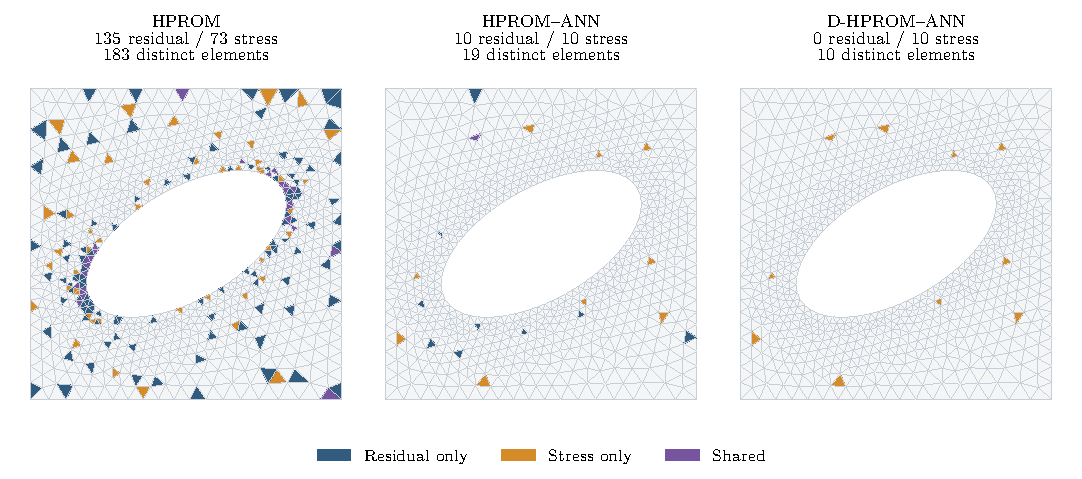
\includegraphics[width=1.75cm,trim=10bp 34bp 348bp 48bp,clip]
      {reduced_supports.pdf}};
 \node[font=\scriptsize,align=center] (hrules) at (2.67,4.96)
   {fixed residual/stress rules\\[-.08em]
    \textcolor{black!58}{$\approx4\%$ of FOM elements}};
 \node[card,minimum width=3.48cm,minimum height=.88cm]
   (hsolve) at (2.67,4.10) {};
 % The residual-vector heights mirror the solved coordinate dimensions.
 \draw[affineblock,rounded corners=.7pt]
   (1.16,3.83) rectangle (1.48,4.43);
 \node[font=\tiny] at (1.32,4.13)
   {$\scriptscriptstyle\bm r_h$};
 \node[font=\tiny,text=black!58] at (1.32,3.76) {$n_{\rm tra}$};
 \node[font=\scriptsize,align=center] at (2.92,4.12)
   {projected equilibrium\\[-.08em]
    $\bm r_h(\qq_{\rm tra};\ee)=\bm0$};

 \node[panel,minimum width=4.72cm,minimum height=4.55cm]
   (hpanncol) at (8.05,5.83) {};
 \node[font=\small\bfseries] at (8.05,7.87)
   {HPROM--ANN};
 \node[card,minimum width=3.48cm,minimum height=.55cm] (haroute)
   at (8.05,7.32) {\scriptsize nonlinear decoder};
 \node[inner sep=0pt] (hasupport) at (8.05,6.09)
   {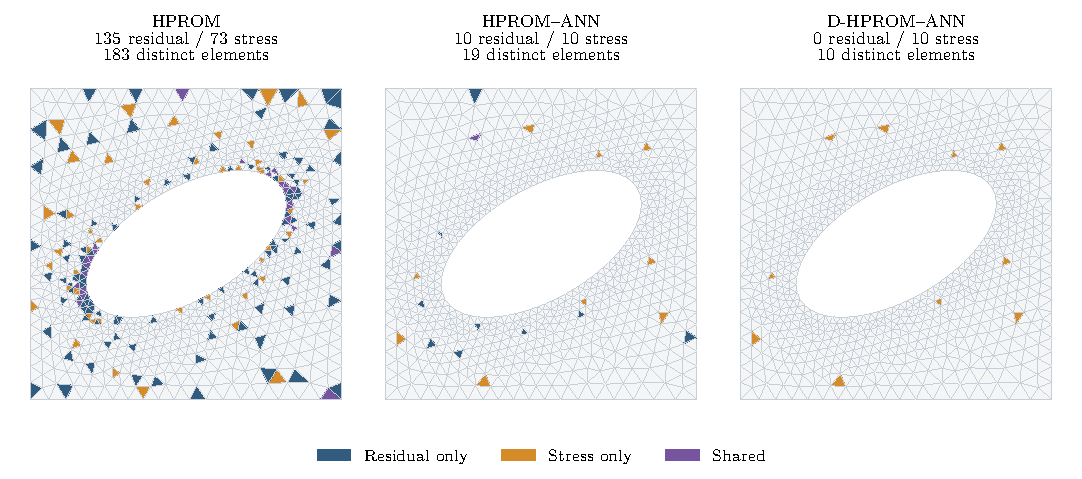
\includegraphics[width=1.75cm,trim=180bp 34bp 175bp 48bp,clip]
      {reduced_supports.pdf}};
 \node[font=\scriptsize,align=center] (harules) at (8.05,4.96)
   {adaptive residual/stress rules\\[-.08em]
    \textcolor{black!58}{$\approx0.4\%$ of FOM elements}};
 \node[card,minimum width=3.48cm,minimum height=.88cm]
   (hasolve) at (8.05,4.10) {};
 \draw[coordprimary,line width=.65pt,rounded corners=.7pt]
   (6.54,3.96) rectangle (6.86,4.30);
 \node[font=\tiny] at (6.70,4.13)
   {$\scriptscriptstyle\bm r_h$};
 \node[font=\tiny,text=black!58] at (6.70,3.81) {$n$};
 \node[font=\scriptsize,align=center] at (8.30,4.12)
   {projected equilibrium\\[-.08em]
    $\bm r_h(\qq;\ee)=\bm0$};

 \node[panel,minimum width=4.72cm,minimum height=4.55cm]
   (dhpanncol) at (13.43,5.83) {};
 \node[font=\small\bfseries] at (13.43,7.87)
   {D-HPROM--ANN};
 \node[card,minimum width=3.48cm,minimum height=.55cm] (droute)
   at (13.43,7.32) {\scriptsize direct decoder, $\bm\xi=\ee$};
 \node[inner sep=0pt] (dsupport) at (13.43,6.09)
   {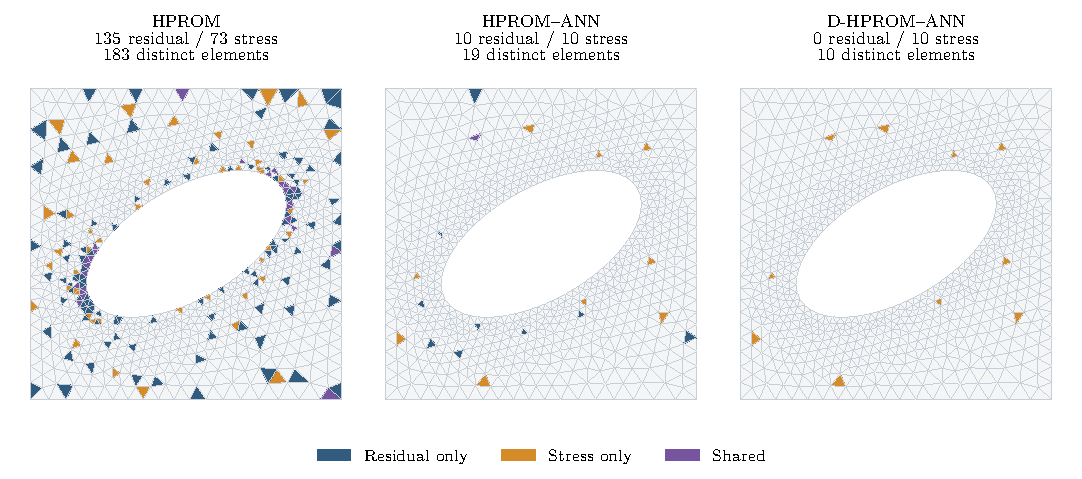
\includegraphics[width=1.75cm,trim=355bp 34bp 5bp 48bp,clip]
      {reduced_supports.pdf}};
 \node[font=\scriptsize,align=center] (drules) at (13.43,4.96)
   {adaptive stress rule\\[-.08em]
    \textcolor{black!58}{$\approx0.2\%$ of FOM elements}};
 \node[card,minimum width=3.48cm,minimum height=.88cm,align=center]
   (dsolve) at (13.43,4.10)
   {\scriptsize one-pass state evaluation\\[-.08em]
    \scriptsize $\ee\longmapsto\widetilde{\bm u}_{D}(\ee)$};

 \draw[flowline] (commoninput.south)--(8.05,8.42);
 \draw[flowline] (2.67,8.42)--(13.43,8.42);
 % The common loading enters through the center of each route frame.
 \draw[flow] (2.67,8.42)--(hpromcol.north);
 \draw[flow] (8.05,8.42)--(hpanncol.north);
 \draw[flow] (13.43,8.42)--(dhpanncol.north);
 \foreach \a/\b/\c/\d in {hroute/hsupport/hrules/hsolve,
                             haroute/hasupport/harules/hasolve,
                             droute/dsupport/drules/dsolve} {
   \draw[secondaryflow] (\a.south)--(\b.north);
   \draw[secondaryflow] (\c.south)--(\d.north);
 }

 % -----------------------------------------------------------------------
 % Row 5: common microscopic output interface.
 \node[panel,minimum width=16.10cm,minimum height=2.96cm,anchor=south west]
   (outputpanel) at (0,.05) {};
 \node[stage] at (.36,2.60) {5};
 \node[font=\small\bfseries,anchor=west] at (.74,2.60)
   {Common constitutive output};
 \node[card,minimum width=4.05cm,minimum height=.82cm,align=center]
   (microlaw) at (3.10,1.18)
   {\scriptsize output cubature\\[-.05em]
    \scriptsize $\bm P_h=
      |Y|^{-1}\!\displaystyle\sum_{e\in\mathcal Z_s}v_e\bm P_e$};
 \node[card,minimum width=3.15cm,minimum height=.82cm,align=center]
   (stressout) at (8.15,1.18)
   {\scriptsize work-conjugate stress $\ssv_h$};
 \node[card,minimum width=3.15cm,minimum height=.82cm,align=center]
   (tangentout) at (12.90,1.18)
   {\scriptsize consistent tangent $\bm D_h$};
 \draw[flow] (microlaw.east)--(stressout.west);
 \draw[flow] (stressout.east)--(tangentout.west);
 \draw[flowline] (hsolve.south)--(2.67,3.18);
 \draw[flowline] (hasolve.south)--(8.05,3.18);
 \draw[flowline] (dsolve.south)--(13.43,3.18);
 \draw[flowline] (2.67,3.18)--(13.43,3.18);
 % Enter below the heading so that the common route does not cross its text.
 \draw[flow,rounded corners=2pt]
   (8.05,3.18)--(8.05,2.10)--(3.10,2.10)--(microlaw.north);
 \node[font=\tiny,text=black!58] at (8.05,.24)
   {same FE$^2$ interface; different state, integration, and equilibrium approximations};
\end{tikzpicture}

 \caption{Intrusive HPROMs used in the comparison. FOM snapshots provide either an affine state representation or a primary--secondary partition in which the ANN predicts the secondary coordinates. Online, HPROM and HPROM--ANN solve projected equilibrium with fixed and adaptive cubature, respectively, whereas D-HPROM--ANN evaluates the nonlinear decoder directly. All three retain microscopic constitutive evaluations and return the same stress--tangent interface.}
\label{fig:reduced_model_hierarchy}
\end{figure}


\subsection{Mechanical structure retained by the HPROMs}
Every HPROM, unlike a direct constitutive surrogate, evaluates the original microscopic hyperelastic law, and the iterative variants also enforce projected equilibrium. Even so, the deployed macroscopic stress need not be the derivative of an effective potential. For fixed weights and consistent kinematics, Galerkin internal forces derive from a weighted reduced energy, as in the structure-preservation results for ECSW~\cite{farhat2015}. Here, however, equilibrium and stress use separate cubature rules, and state-dependent weights add the term $\sum_e\Pi_e\nabla_{\qq}w_e$ to the gradient of the weighted energy $\sum_e w_e(\qq)\Pi_e(\qq,\ee)$, a term that Eq.~\eqref{eq:maw} omits. Consequently, no exact effective potential or polyconvexity certificate is claimed for the HPROMs, whose consistent tangent is the derivative of the implemented stress map and need not be symmetric.

Table~\ref{tab:reduction_levels} summarizes the three HPROMs and their FOM reference.

\begin{table}[htbp]
 \centering\small
 \caption{HPROMs used in the accuracy--cost comparison and their FOM reference. All HPROMs retain microscopic constitutive evaluations.}
 \label{tab:reduction_levels}
 \setlength{\tabcolsep}{4pt}
 \renewcommand{\arraystretch}{1.2}
 \begin{tabularx}{\linewidth}{@{}llcYY@{}}
 \toprule
 Model & State representation & \begin{tabular}[t]{@{}c@{}}Equilibrium\\unknowns\end{tabular} & Integration & Learned component\\
 \midrule
 FOM & $\bm u$ & $N$ & Full mesh & None\\
 \addlinespace[.3em]
 HPROM & $\widetilde{\bm u}=\bm u_{\rm ref}+\bm V_{\rm tra}\qq_{\rm tra}$ & $n_{\rm tra}$ & Fixed ECM (residual and stress) & None\\
 \addlinespace[.3em]
 HPROM--ANN & $\widetilde{\bm u}(\bm\xi)=\bm u_{\rm ref}+\bm V\bm A_m\bm\xi+\overline{\bm V}\widehat{\mathcal N}(\bm\xi)$ & $n$ & Adaptive ECM (residual and stress) & Secondary coordinates; residual and stress weights\\
 \addlinespace[.3em]
 D-HPROM--ANN & $\widetilde{\bm u}_{D}(\ee)=\bm u_{\rm ref}+\bm V\bm A_m\ee+\overline{\bm V}\widehat{\mathcal N}(\ee)$ & None & Adaptive ECM (stress only) & Same closure and stress weights as HPROM--ANN\\
 \bottomrule
 \end{tabularx}
\end{table}
\FloatBarrier


\section{Numerical examples}
\label{sec:cell}
We use two periodic microstructures, each with its own independently trained models, so that the assessment does not rest on a single cavity arrangement. The multicavity RVE (MC-RVE) presents several geometric directions within one cell, which makes it a natural setting in which to isolate the effect of learning the paired features and of changing their number. The single-cavity RVE (SC-RVE) is instead the microscopic model subsequently propagated through the structural FE$^2$ calculation and shared with the intrusive references of Section~\ref{sec:reduced}; it therefore supplies the deployment qualification. Together, the two benchmarks test the same constitutive construction in distinct geometric settings, but not transfer of parameters between them.

The evidence follows those roles in causal order. After the common setting, we first ask on the MC-RVE how many paired features are needed and what learning them adds. We then ask on the SC-RVE whether the selected learned energies are accurate enough for the structural calculation of Section~\ref{sec:coupon}. Throughout, analytical guarantees are distinguished from predictive accuracy and finite implementation checks.

\subsection{Common setting}
Both benchmarks are square periodic cells with total void fraction $0.20$.  Their solid phase follows the same compressible Neo-Hookean law in plane strain.  With $\C_\mu=\F_\mu^T\F_\mu$ and $J_\mu=\det\F_\mu>0$, its local energy density is
\begin{equation}
 \psi_\mu=\frac\mu2(\tr\C_\mu-2)-\mu\log J_\mu
              +\frac\lambda2(\log J_\mu)^2,
\end{equation}
with Young's modulus $1.628$ GPa and Poisson ratio $0.4$, where $\mu$ and $\lambda$ are the Lam\'e constants.  The cavity geometry, rather than the matrix law, distinguishes the two benchmarks.

\paragraph{A common diagnostic state.}
The two cells respond differently to the same multiaxial deformation.  Figure~\ref{fig:common_rve_fields} applies $(E_{11},E_{22},2E_{12})=(18,-4,8)\%$ to both FOMs.  The inclined cavity of the SC-RVE concentrates the response around one dominant geometric direction, whereas the nonaligned cavities of the MC-RVE create several interacting localization regions.  This geometric contrast motivates the distinct roles of the two benchmarks; the figure shows FOM fields only and is not an error test.

\begin{figure}[t]
 \centering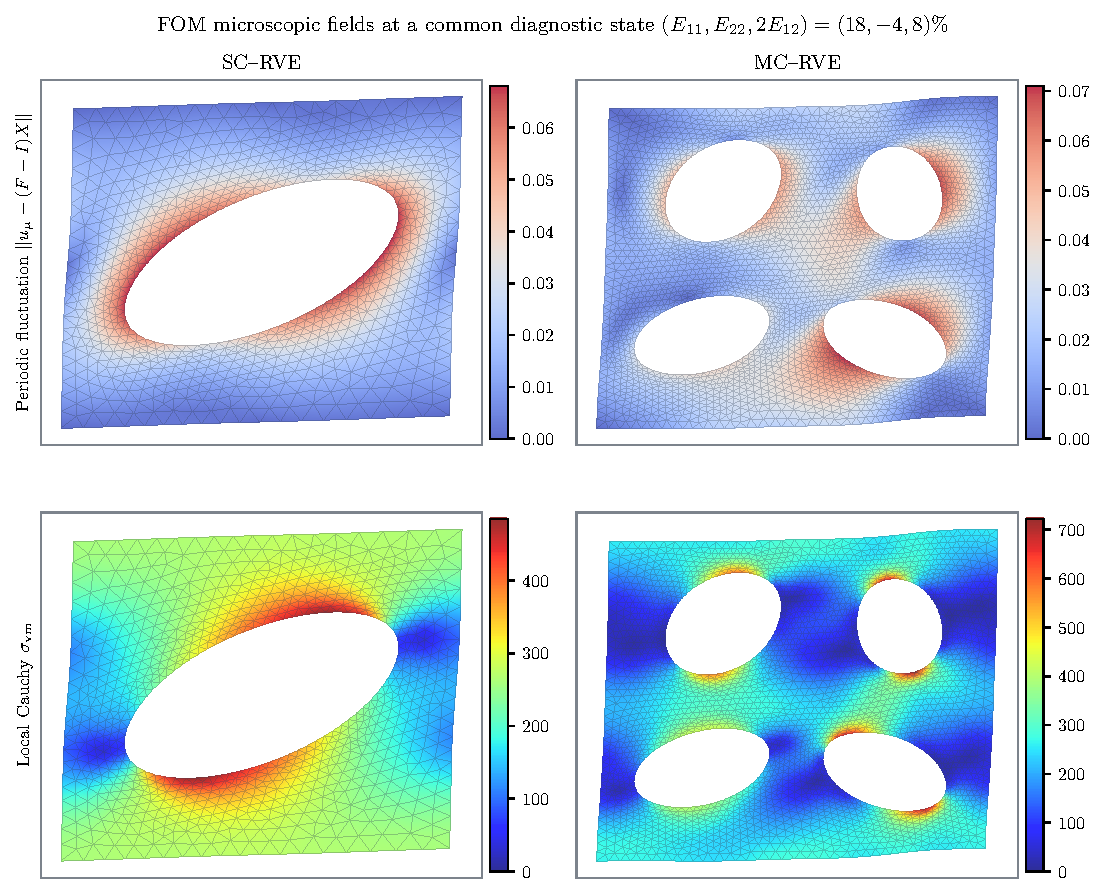
\includegraphics[width=.97\linewidth]{rve_common_diagnostic_fields.pdf}
 \caption{FOM microscopic fields at the common diagnostic state $(E_{11},E_{22},2E_{12})=(18,-4,8)\%$, shown on the actual deformed cells without displacement amplification.  Top: magnitude of the periodic displacement fluctuation after removing the imposed affine part.  Bottom: local three-dimensional Cauchy von Mises stress, including the plane-strain out-of-plane stress; Gauss-point values are averaged to the nodes for visualization.  Each panel uses its own color limits to resolve the spatial pattern within its respective cell; colors are therefore not a cross-cell magnitude comparison.}
 \label{fig:common_rve_fields}
\end{figure}

\subsubsection{Training protocol}
\label{sec:training_protocol}
The two benchmarks answer different questions, but their energies are trained and selected in the same way, so that differences within each benchmark reflect the constitutive representation rather than the fitting procedure.  Every model is a scalar energy $W(\ee;\bm\theta)$, whose first derivative gives the stress and whose second derivative gives the tangent $\bm D$ of Eq.~\eqref{eq:tangent}.  It is fitted to FOM energies and stresses at the fitting states and to the effective tangent $\bm D_0=\bm D(\bm 0)$ of the periodic cell at the undeformed state.

The ICNN of Eq.~\eqref{eq:monotone_icnn} and the ICKAN of Eq.~\eqref{eq:monotone_ickan} have two hidden layers of widths 24 and 12, respectively, and each ICKAN connection combines six integrated-hat bases on fixed knots from $-1.2$ to $1.2$ ($h=0.48$).  With six fixed paired features, the ICNN has 945 trainable parameters and the ICKAN 1629; learning the features adds only five parameters per feature.  The initial features are selected from a finite bank of admissible candidates using only the fitting response and the reference tangent.\footnote{The bank contains 2028 candidates, which combine twelve orientations $\theta_i=k\pi/12$ with the stretch powers $p_i,q_i\in\{0.5,1,1.5,2,3\}$ and with determinant exponents at the bounds and midpoint of Eq.~\eqref{eq:featureconstraints}, moved slightly inside the admissible interval so that the parameterization of Eq.~\eqref{eq:feature_parameterization} can represent them.  Nonnegative least-squares fits of the fitting response and of the reference tangent identify the contributing candidates.  The largest contributions are retained when more than $m$ are selected, and pivoted QR completes the set when fewer are.}  Before entering either core, each feature is centered at its undeformed value $z_i^0=1/p_i+1/q_i$ and divided by its largest deviation from that value over the fitting states at initialization.  The conditioned inputs therefore start in $[-1,1]$, which the ICKAN knots cover with a small margin.  The Unconstrained energy uses three softplus hidden layers of widths 128, 128, and 64 on the inputs of Eq.~\eqref{eq:unconstrained_inputs}, for 25\,473 parameters.

All trainable parameters, including the feature parameters of the learned variants, minimize
\begin{equation}
 \mathcal L(\bm\theta)=
 \frac{\sum_k\|\ssv(\ee_k;\bm\theta)-\ssv_k\|_2^2}{\sum_k\|\ssv_k\|_2^2}
 +0.2\,\frac{\sum_k\bigl[W(\ee_k;\bm\theta)-W_k\bigr]^2}{\sum_k W_k^2}
 +0.02\,\frac{\|\bm D(\bm0;\bm\theta)-\bm D_0\|_F^2}{\|\bm D_0\|_F^2},
 \label{eq:training_loss}
\end{equation}
where the sums run over the fitting states $\ee_k$, with FOM energies $W_k$ and stresses $\ssv_k$.  Stress carries the largest weight because it is queried throughout the FE$^2$ calculation.  The energy term keeps the potential itself, and not only its gradient, close to the homogenized energy.  The small tangent term anchors the stiffness at the undeformed state, where the vanishing stresses contribute little to the first term.

Optimization is full-batch and in double precision.  The validation error is the first term of Eq.~\eqref{eq:training_loss} evaluated on the validation states.  Adam runs until this error stops improving, or for at most 200\,000 steps, and L-BFGS then refines the best Adam state.\footnote{Adam starts from learning rates of $5\times10^{-3}$ for the ICNN and ICKAN and $4\times10^{-4}$ for the Unconstrained energy, halved after 40 validation checks without improvement down to $10^{-5}$, with a check every ten steps.  It stops when the best validation error improves by less than $0.1\%$ over 100 checks at the smallest learning rate.  L-BFGS, in calls of at most ten iterations, stops under the same criterion over 30 calls.}  The retained checkpoint is the one with the lowest validation error, and each model is trained from three seeds, 16, 29, and 47.  Independent test states are evaluated only after every checkpoint has been frozen.
\FloatBarrier

\subsection{Multicavity RVE: learning the paired features}
\label{sec:constitutive_training}
The paired-feature construction guarantees admissibility for every allowed parameter set, but it does not determine how much directional information the convex core needs.  This question is particularly relevant for the MC-RVE, whose nonaligned cavities introduce several geometric directions.  A small prescribed feature set may then fail to distinguish deformation states with different directional responses.  One remedy is to supply more features; another is to let their directions and exponents adapt to the RVE response.  We examine both effects together by asking how accuracy changes with the number $m$ of paired features and, for each $m$, what is gained by learning rather than fixing their parameters.

\subsubsection{Cell, data, and controlled comparison}
\label{sec:material_b}
The MC-RVE distributes the void space among four unequal, off-center ellipses with different aspect ratios and orientations; see Fig.~\ref{fig:rve_b}.  Its several geometric directions make it the representation benchmark.  The working mesh has 4621 quadratic triangles.

\begin{figure}[htbp]
 \centering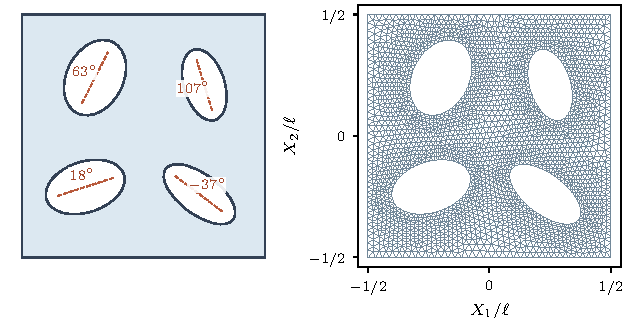
\includegraphics[width=.96\linewidth]{rve_geometry_b.pdf}
 \caption{MC-RVE cavity geometry (left) and quadratic mesh (right).  Dashed lines identify cavity major axes.}
 \label{fig:rve_b}
\end{figure}

Refining the mesh to 8961 elements changes the homogenized energy, stress, and tangent by less than $0.1\%$ over 64 audited states that include the corners of the strain domain used below; the sampled maximum microscopic first Piola stress norm changes by at most $4.06\%$.  These comparisons support the working mesh for the representation study.

\paragraph{Controlled comparison.}
We sample $E_{11},E_{22}\in[-0.04,0.20]$ and $2E_{12}\in[-0.08,0.08]$.  The left panel of Fig.~\ref{fig:constitutive_domains} shows the domain.  The 4200 fitting states combine 4096 scrambled Sobol points in the interior with 96 points on the faces and the eight corners, so that the boundary of the box is sampled rather than reached by extrapolation.  Independent Sobol sequences supply 512 validation and 512 independent-test states.  Ten further straight paths run from the undeformed state to the boundary of the box in axial, biaxial, shear, and combined directions, each with 40 scored states; like the test states, they play no role in training or selection.  For each $m\in\{2,4,6,8,16,24,32\}$, ICNN and ICKAN are trained in two variants that start from the same $m$ initial features.  The fixed variant holds their directions and exponents constant while training the convex core, whereas the learned variant optimizes those parameters subject to the constraints of Section~\ref{sec:learned}.  All other ingredients of Section~\ref{sec:training_protocol} are shared within each core, so the difference between the two variants isolates the effect of adapting the features.

\begin{figure}[htbp]
 \centering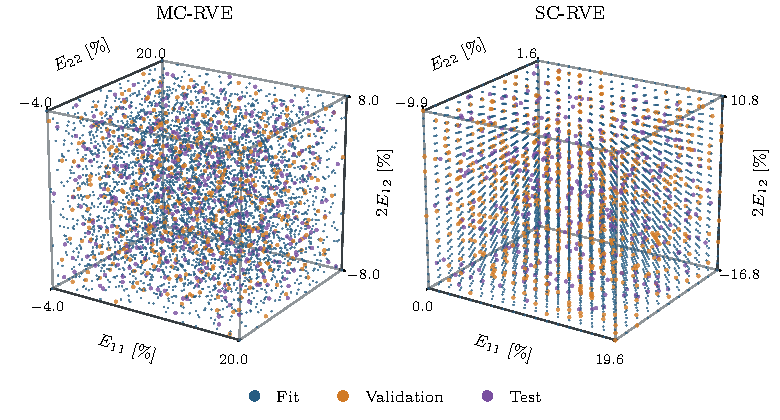
\includegraphics[width=.98\linewidth]{constitutive_domains.pdf}
 \caption{Constitutive sampling domains, in percent.  Left: MC-RVE representation benchmark.  Right: SC-RVE deployment benchmark.  Wireframes show the prescribed limits; colors identify fitting, validation, and independent-test states.}
 \label{fig:constitutive_domains}
\end{figure}

\subsubsection{How many paired features are needed?}
Figure~\ref{fig:feature_count_sensitivity} answers this question in the same way for both convex cores.  Two paired features leave the response under-resolved, and both variants improve as $m$ increases, but in different ways.  The learned variants gain most up to $m=6$ and change by less than a factor of two beyond it, whereas the fixed variants continue to improve gradually up to $m=32$.  We therefore select $m=6$, the first count at which both learned cores enter their low-error regime, for independent evaluation.

\begin{figure}[htbp]
 \centering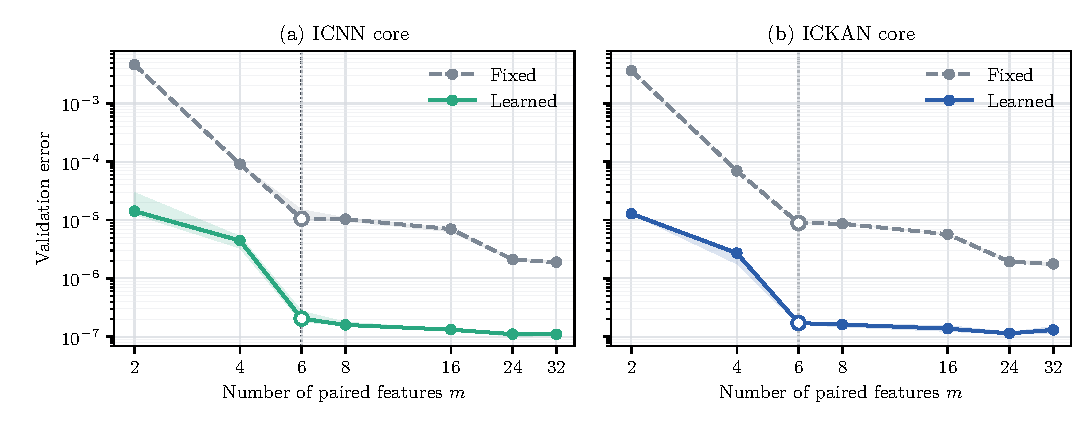
\includegraphics[width=.98\linewidth]{feature_count_sensitivity.pdf}
 \caption{MC-RVE validation error, the relative squared stress error of Section~\ref{sec:training_protocol}, versus the number $m$ of paired directional features.  Lines show the median over three seeds and bands span their minimum--maximum range.  The vertical guide marks $m=6$, used for the independent comparison.}
 \label{fig:feature_count_sensitivity}
\end{figure}

\subsubsection{What does learning the features add?}
Table~\ref{tab:mc_rve_m06} answers this question on the independent test states.  At $m=6$, learning the paired features lowers the ICNN median stress error from $0.328\%$ to $0.0445\%$ and the ICKAN error from $0.301\%$ to $0.0406\%$, a reduction by a factor of approximately $7.4$ in either core.  The energy and the tangent, which is never fitted away from the undeformed state, improve by factors of about 14 and 5, respectively.  Adding prescribed directions does not close this gap.  In the validation sweep, even 32 fixed features, with more than twice the trainable parameters of the learned six-feature models, remain about three times less accurate in relative stress error, a factor of about ten in the squared validation error of Fig.~\ref{fig:feature_count_sensitivity}.  The ten held-out paths confirm the ordering for stress, energy, and tangent on every path.  The largest gain appears in pure shear, where the relative stress error falls from $3.2$--$4.0\%$ with fixed features to $0.47$--$0.58\%$ with learned ones, whereas biaxial compression produces the largest tangent errors for both variants.  The similar gain for ICNN and ICKAN shows that the central improvement comes from adapting the directional representation rather than from one particular convex core.

The Unconstrained energy places these values in context.  Without convexity or growth conditions, it reaches $0.0073\%$ on the same states, about six times below either learned constrained model.  Its network is also considerably larger.  At matched capacity, the controls of Appendix~\ref{app:capacity} place the in-domain cost of the constraints on this cell at a factor of 3.2 to 5.5 in stress error; the one exception, a wide ICKAN, reflects early stopping rather than capacity.

\begin{table}[htbp]
 \centering\small
 \caption{MC-RVE independent-test errors at $m=6$.  Each entry is the relative error norm of the stress $\ssv$, the energy $W$, or the tangent $\bm D$ of Eq.~\eqref{eq:tangent} over the 512 test states, as the median over three seeds.  For every quantity, each learned seed is more accurate than each fixed seed.  Adam stopped at a validation plateau for the fixed variants, whereas five of the six learned runs and the Unconstrained energy, which has no paired features, reached the 200\,000-step cap.}
 \label{tab:mc_rve_m06}
 \begin{tabular}{lccc}
\toprule
Model & Stress [\%] & Energy [\%] & Tangent [\%]\\
\midrule
ICNN, fixed & 0.3282 & 0.1096 & 1.9247\\
ICNN, learned & 0.0445 & 0.0079 & 0.3851\\
\addlinespace
ICKAN, fixed & 0.3014 & 0.0943 & 1.7600\\
ICKAN, learned & 0.0406 & 0.0066 & 0.3622\\
\midrule
Unconstrained energy & 0.0073 & 0.0011 & 0.0857\\
\bottomrule
\end{tabular}

\end{table}

\subsubsection{What do the constraints guarantee beyond the data?}
\label{sec:mc_guarantees}
For the ICNN and ICKAN energies, conditions (C1)--(C6) hold for every admissible parameter set by construction, whereas the Unconstrained energy is built to satisfy (C1)--(C4) only.  Inside the box the difference does not show, since a bounded rank-one search over 520 states and 32 directions finds curvature above 236~MPa for all fifteen fits of Table~\ref{tab:mc_rve_m06}.  Farther out the two classes separate.  Figure~\ref{fig:mc_beyond_data}(a) follows equibiaxial compression, $\F=\sqrt J\,\I$, beyond the box.  The minimum rank-one curvature of every Unconstrained fit changes sign between $J=0.71$ and $0.73$, whereas the learned constrained fits remain above 220~MPa.  A directed search over principal stretches between 0.55 and 1.5, in arbitrary orientations, shows that this loss is not tied to one path.  It finds negative curvature for all three Unconstrained fits at more than a third of its 4096 sampled states, confirmed by energy finite differences, and only positive curvature for the twelve constrained fits, as their construction requires.

Figure~\ref{fig:mc_beyond_data}(b) continues the same path toward volume collapse.  The constrained energies diverge, as their logarithmic barrier guarantees, whereas the Unconstrained energy levels off at finite limits between 397 and 440~MPa.  This contrast reflects the growth terms rather than polyconvexity, and an unconstrained network could receive the same barrier.  No data constrain either energy at these states, so only the construction can guarantee (C5) and (C6) there.

\begin{figure}[htbp]
 \centering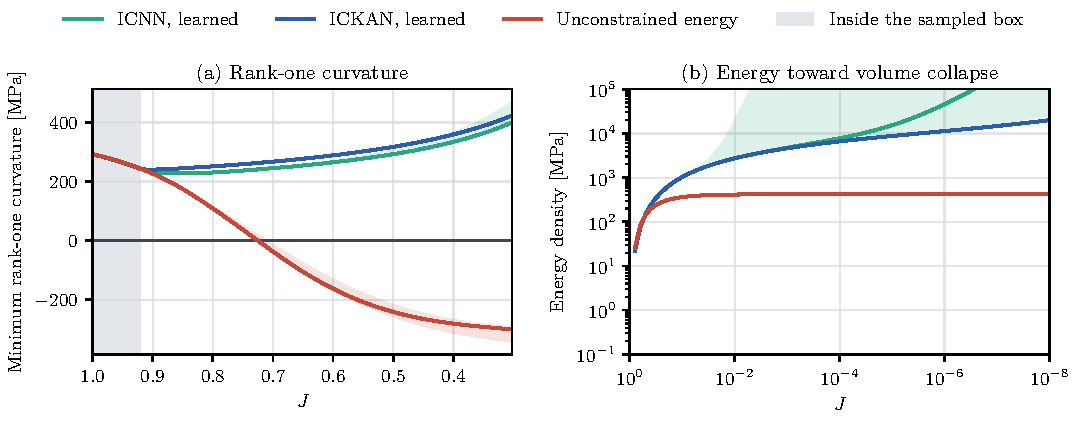
\includegraphics[width=.98\linewidth]{mc_beyond_data.pdf}
 \caption{MC-RVE energies beyond the data along equibiaxial compression, $\F=\sqrt J\,\I$, for the learned ICNN and ICKAN energies and the Unconstrained energy.  Lines show the median of three seeds and shaded bands their range.  (a) Minimum rank-one curvature over unit directions.  (b) Energy density toward volume collapse.}
 \label{fig:mc_beyond_data}
\end{figure}

Global nonnegative energy, which the construction leaves to the saved parameters, is certified by the sufficient bound of Appendix~\ref{app:nonnegative} for all six learned fits, with interval margins between 8.5 and 10.8 in normalized energy units.  For all fifteen fits, the reference energy and stress vanish to round-off, and centered differences reproduce the stress and the tangent to better than $10^{-9}$ of their largest entries.

Taken together, the MC-RVE supports the choices carried into the SC-RVE study.  Six paired features give a compact representation, and adapting their directional parameters supplies the main accuracy gain for either convex core.  The learned constrained energies then keep the median stress error below $0.05\%$ while securing, beyond the data, the rank-one convexity and growth that the Unconstrained energy loses there.
\FloatBarrier

\subsection{Single-cavity RVE: constitutive accuracy and FE$^2$ deployment}
\subsubsection{Cell and coupon-derived data}
\label{sec:material_a}
The SC-RVE contains one centered elliptical void with aspect ratio $2$ and major-axis angle $30^\circ$ relative to the cell axes; see Fig.~\ref{fig:rve}.  Its working mesh has 1546 quadratic triangles and 6320 independent microscopic displacement coordinates.

\begin{figure}[htbp]
 \centering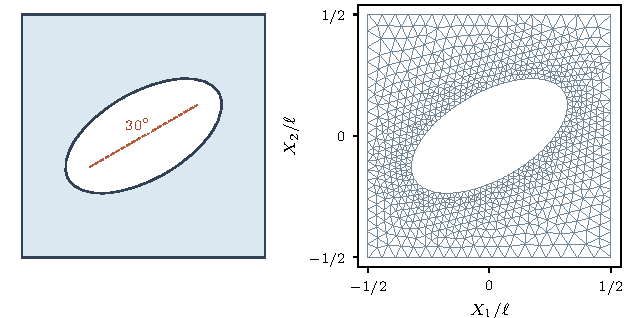
\includegraphics[width=.96\linewidth]{rve_geometry.pdf}
 \caption{SC-RVE cavity geometry (left) and quadratic mesh (right).  The dashed line identifies the cavity major axis.}
 \label{fig:rve}
\end{figure}

At a uniaxial-stress state with $E_{11}=0.20$, refining the mesh to 3095 elements changes the maximum microscopic first Piola stress norm by approximately $0.486\%$ and the average axial stress by approximately $0.001\%$.  This state lies on the path followed by the narrow section of the coupon in Section~\ref{sec:coupon}, beyond the largest axial strain reached there, so the check supports the mesh used for deployment.

\paragraph{Coupon-derived data.}
Unlike the MC-RVE, whose box is prescribed, the SC-RVE must supply the learned constitutive response throughout the coupon FE$^2$ calculation of Section~\ref{sec:coupon}, whose macroscopic quadrature points visit different strains during loading.  We first ran a displacement-controlled coupon prepass with a St Venant--Kirchhoff approximation based on the cell reference tangent.  The recorded strain envelope guides sampling only; RVE stresses provide the training labels.  A second prepass with a softer response shifted the componentwise extrema by at most $5.1\%$, so we enlarged the spans by $40\%$.  Because the coupon is tensile, the lower $E_{11}$ bound is zero.  In the engineering-strain coordinates $\ee=(E_{11},E_{22},2E_{12})^T$, the rounded bounds are
\begin{equation}
 \ee_{\min}=(0,-0.099,-0.168)^T,\qquad
 \ee_{\max}=(0.196,0.016,0.108)^T.
 \label{eq:box}
\end{equation}
A Cartesian grid supplies 4950 nonreference states, of which 4208 are used for fitting and 742 for validation (split seed 5); an independent off-grid set of 400 states tests interpolation; see the right panel of Fig.~\ref{fig:constitutive_domains}.  The same grid also provides neighboring states for the reduced microscopic models of Section~\ref{sec:reduced}.

\subsubsection{Constitutive accuracy}
\label{sec:constitutive_accuracy}
The MC-RVE study identifies $m=6$ as the first compact count at which both learned cores enter their low-error regime.  We therefore ask whether that same count is sufficient for the SC-RVE deployment, without transferring feature parameters between the two geometries.  Six initial features are selected anew from the SC-RVE fitting response and reference tangent, and the learned ICNN and ICKAN are trained as described in Section~\ref{sec:training_protocol}, as is the Unconstrained energy.  For each model, the seed with the lowest validation error supplies the deployed model.  Both constrained selections fall on seed 16, with the validation errors of the three seeds within $15\%$ of one another, and the Unconstrained selection falls on seed 47.

\paragraph{Independent response.}
The 400 off-grid states now answer the deployment question directly.  The compact ICNN and ICKAN attain aggregate stress errors of $0.621\%$ and $0.636\%$, respectively, and the Unconstrained energy reaches $0.0052\%$, about 120 times lower; see Table~\ref{tab:constitutive}.  On this cell the construction therefore costs far more accuracy than on the MC-RVE, and capacity is not the reason.  In the controls of Appendix~\ref{app:capacity}, cores widened to about 25\,000 parameters change the constrained errors by less than $3\%$, whereas an Unconstrained energy with only 981 parameters remains about 75 to 80 times more accurate than either wide core.  Thirty-two learned features lower the errors only to $0.537\%$ and $0.618\%$.  This behavior is consistent with the ordering argument of Section~\ref{sec:feature_order}, since a monotone core cannot reverse the componentwise ordering of its features whatever its width; widening the core therefore cannot enlarge the response family beyond what the features and that ordering admit.  The price of this restriction depends on the cell, a factor of 3.2 to 5.5 on the MC-RVE and of 76 to 126 on the SC-RVE at matched capacity.  Comparable costs are reported for other constrained constructions.  Linden et al.~\cite{linden2023} found that imposing all common conditions on a small invariant-based network raised its stress error by about one order of magnitude for transverse isotropy, and still recommended the constrained model for its extrapolation.  On homogenization data of a matrix with a stiff spherical inclusion, the polyconvex models of Klein et al.~\cite{klein2026} reached root-mean-square stress errors three to five times those of their non-polyconvex counterparts, and Kalina et al.~\cite{Kalina2024} dropped polyconvexity after finding it too restrictive for their fits.  The MC-RVE factors are of this size, whereas the SC-RVE shows that the price can be much larger for some microstructures.

\paragraph{Response beyond the box.}
A separate 350-state probe resolves the response outside the fitting box.  It contains five increasing overshoot factors and labelled face, edge, and corner patterns; five states without a finite FOM label are excluded for every model, leaving 345.  The aggregate probe errors rise to $10.6\%$ and $10.1\%$ for ICNN and ICKAN and to $0.668\%$ for the Unconstrained energy, with the ringwise results in Supplementary Section~S1.  On this cell the constraints thus cost accuracy inside and outside the box.  Inside it, where every coupon state lies, both constrained energies remain below $0.65\%$; what the constraints secure beyond it is examined next.  Thirty-two features would also raise the probe errors to $35.6\%$ and $16.9\%$ and lose the nonnegative-energy certificate of Appendix~\ref{app:nonnegative}, so the coupon keeps the $m=6$ models.

\begin{table}[htbp]
 \centering\small
 \caption{SC-RVE independent-test constitutive errors of the selected models, in percent.}
 \label{tab:constitutive}
 \begin{tabular}{lrr}
\toprule
Model & $e_S^{\rm test}$ [\%] & $e_W^{\rm test}$ [\%] \\
\midrule
HPROM & 0.0169 & -- \\
HPROM--ANN & 0.2177 & -- \\
D-HPROM--ANN & 0.0959 & -- \\
ICNN & 0.6214 & 0.1929 \\
ICKAN & 0.6359 & 0.1900 \\
Unconstrained energy & 0.0052 & 0.0010 \\
\bottomrule
\end{tabular}

\par\smallskip{\footnotesize All values are percentages. Stress and energy errors are aggregate array norms. SC-RVE: 400 independent test states. The HPROMs return no energy.}

\end{table}
\FloatBarrier

\subsubsection{Admissibility beyond the data}
\label{sec:mechanical_assessment}
The comparison of Section~\ref{sec:mc_guarantees} carries over to this cell; Supplementary Section~S2 gives the sampled values.  On the test, probe, and 12\,000 additional in-box states, the rank-one curvature of all three energies stays above 135~MPa.  Farther out, a radial expansion of the box to four times its size finds negative curvature for the Unconstrained energy at 14\,108 of 109\,743 states, first at 1.55 times the box and $J=0.78$, and a broad scan of principal stretches between 0.25 and 3 finds it at 10\,048 of 24\,000 states.  The ICNN and ICKAN remain above 176~MPa on both sets.  The Unconstrained energy also stays finite along $\F=\sqrt J\,\I$ as $J\to0^+$, because its network inputs remain bounded on that path, whereas the logarithmic barrier makes the constrained energies diverge.  For the two deployed models, the sufficient bound of Appendix~\ref{app:nonnegative} certifies nonnegative energy, with interval margins of 4.85 and 4.91 in normalized energy units.  For all three energies, derivative checks and the vanishing closed-cycle work of Supplementary Section~S3 confirm the potential structure of the implementation.
\FloatBarrier

\subsubsection{Reduced models built from the same snapshots}
\label{sec:material_a_reduction}
The 4950 displacement snapshots provide the basis of the reduced microscopic models as well as the effective constitutive labels. Figure~\ref{fig:pod} shows how the relative truncation norm of their POD basis decays with the number of modes; for the retained 39-dimensional space it is $9.94\times10^{-7}$. After its orthogonal rotation into primary and secondary spaces, $n=3$ and $\bar n=36$ in the notation of Section~\ref{sec:reduced}.

The fitted relation between the deployed primary coordinates and macroscopic strain has an aggregate relative array discrepancy of $3.60\times10^{-5}$ on these snapshots; its maximum absolute component discrepancy is $2.55\times10^{-5}$. These quantities explain why macroscopic strain is a useful primary-coordinate predictor for this material. The direct substitution in D-HPROM--ANN nevertheless remains an additional approximation.

The secondary-coordinate closure is a $3$--$64$--$64$--$36$ feed-forward network with two $\tanh$ hidden layers and a linear output. Its training script uses input standardization, the raw secondary-coordinate loss in Eq.~\eqref{eq:closure_loss}, and a 90/10 internal fit/validation split with seed 20260903. Full-batch Adam has initial learning rate $2\times10^{-3}$, a validation-driven reduction schedule, and a maximum budget of 20000 epochs. Its best relative validation mean-square error is $3.75\times10^{-7}$, an internal closure metric; the coupon of Section~\ref{sec:coupon} provides the independent assessment.

Each deployed adaptive cubature field has architecture $3$--$128$--$128$--$128$--$10$, GELU hidden activations, and the scaled softmax output of Eq.~\eqref{eq:softmax_weights}. The residual and stress checkpoints use distinct ten-element supports. Their larger neural cores illustrate why the online cost cannot be inferred solely from the three equilibrium coordinates or from the element count.

\begin{figure}[htbp]
 \centering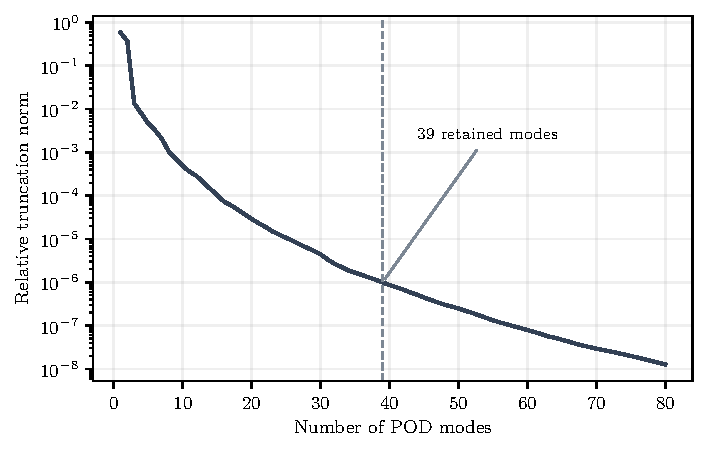
\includegraphics[width=.6\linewidth]{pod_primary_coordinates.pdf}
 \caption{Relative truncation norm of the POD basis of the 4950 SC-RVE displacement snapshots versus the number of modes. The deployed basis retains 39 modes; its rotation into primary and secondary coordinates leaves this span unchanged.}
 \label{fig:pod}
\end{figure}

\paragraph{Online models.}
The linear HPROM uses $n_{\rm tra}=39$ generalized coordinates, a residual rule supported on 135 elements, and a stress rule on 73 elements; their union contains 183 elements. The integrand-SVD tolerances are $\varepsilon_{\rm SVD}^{r}=10^{-3}$ and $\varepsilon_{\rm SVD}^{s}=10^{-5}$, retaining 134 and 72 integrand modes, respectively. The greedy integration tolerance in Eq.~\eqref{eq:ecm_tolerance} is $\varepsilon_{\rm ECM}=10^{-6}$ for both rules, including the multiplier-sum constraint.

The iterative HPROM--ANN uses $n=3$ primary and $\bar n=36$ secondary coordinates, with ten residual and ten stress elements and a union of 19. Initial fixed-ECM candidates use $\varepsilon_{\rm SVD}=10^{-4}$ and $\varepsilon_{\rm ECM}=10^{-6}$; adaptive pruning targets ten elements per rule. This count is a prescribed pruning target, assessed through integration and response errors. The pruning uses up to 500 sampled states, tests up to 20 removal candidates per elimination, and applies only the local, positivity-enforcing stage of the algorithm; the residual weight field is then refitted on the same support with a longer training budget.

The direct model evaluates stress on ten elements and solves no microscopic equilibrium equations. All these counts refer to reduced computational meshes, not full-mesh evaluations followed by masking. Figure~\ref{fig:supports} shows their spatial distribution and the overlap of residual and output rules.

\begin{figure}[htbp]
 \centering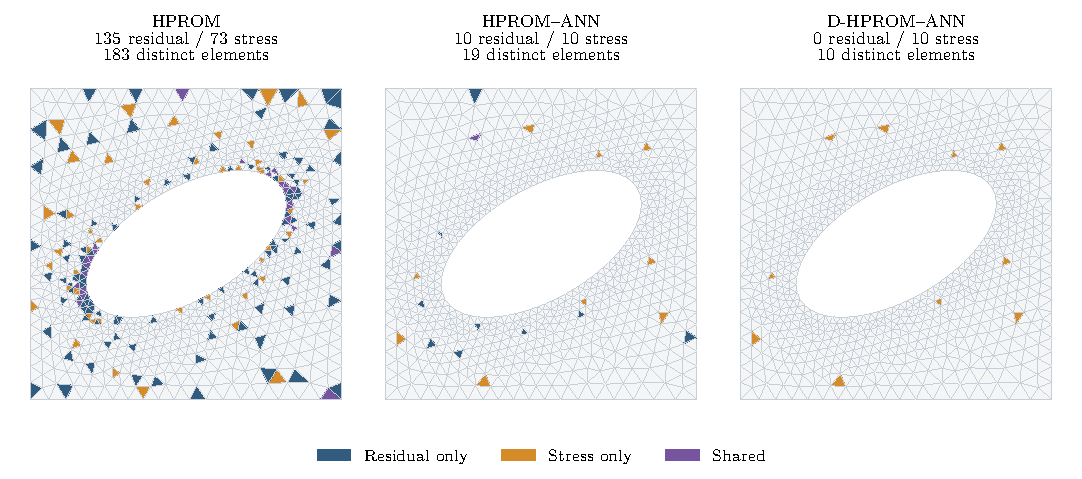
\includegraphics[width=.99\linewidth]{reduced_supports.pdf}
 \caption{Element supports of the deployed hyperreduced microscopic models. The pale full-cell mesh provides location context only; discarded elements are not assembled online. Colors distinguish residual-only, stress-only, and shared elements.}
 \label{fig:supports}
\end{figure}

\subsubsection{Coupon FE$^2$: accuracy and online cost}
\label{sec:coupon}
\paragraph{Purpose, boundary conditions, and coverage.}
We now use the SC-RVE to compare learned constitutive laws and reduced microscopic solvers within the same nonlinear structural calculation. The coupon measures how their approximations affect structural accuracy and online cost. The dog-bone profile has overall length 165 mm, grip width 19 mm, narrow-section width 13 mm, narrow-section length 57 mm, and fillet radius 76 mm. It is a plane-strain computational benchmark using an ASTM-inspired in-plane profile, not a simulation certified to reproduce an ASTM tensile test.

\begin{figure}[htb]
 \centering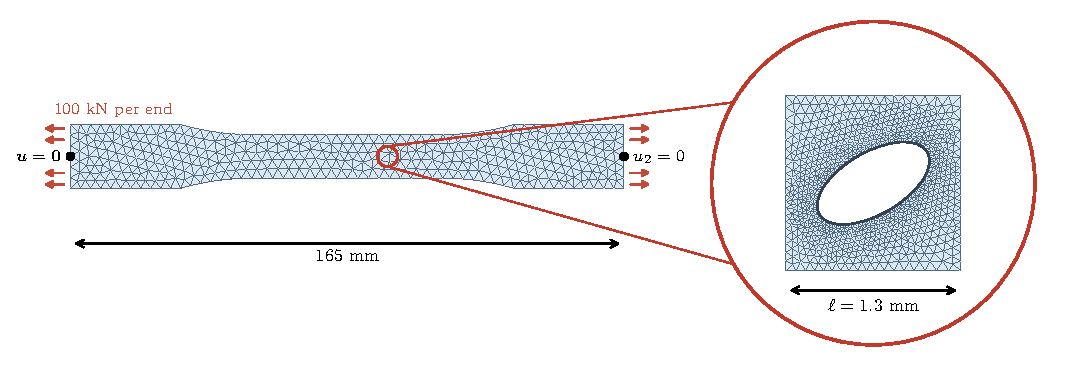
\includegraphics[width=.99\linewidth]{two_scale_coupon.pdf}
 \caption{Coupon problem.  Undeformed macro mesh with equal-and-opposite resultants of 100~kN per end; the three point constraints only remove rigid-body motion, since the two resultants balance each other.  Every integration point queries the SC-RVE, solved by the FOM or replaced by a reduced model or a learned energy.}
 \label{fig:coupon_setup}
\end{figure}

The two end faces receive equal-and-opposite axial resultants of 100 kN per end, applied in 20 equal increments (Fig.~\ref{fig:coupon_setup}). Three point constraints remove rigid modes: the axial and transverse displacement at the left mid-edge node, and transverse displacement at the right mid-edge node. Entire end faces are not clamped. Consequently, a small skew of the deformed ends is not ruled out by the boundary conditions. The anisotropic response can couple axial extension to shear.

The macro mesh contains 690 quadratic triangles, 1501 nodes, and 2070 integration points. The reference extrusion thickness used to convert the two-dimensional stress integrals into the stated force resultants is 50 mm. This force convention is part of the plane-strain benchmark, not an ASTM specimen-thickness specification. The physical cell size is declared as 1.3 mm, corresponding to ten cells across the narrow width. This provides a scale-separation assumption, not a direct numerical validation of homogenization error at that ratio. All saved converged integration-point strains for every reported model remain inside the unchanged training box. Figure~\ref{fig:coupon} shows the reference fields at the final load. The equivalent stress is nearly uniform in the narrow section, peaks slightly where the fillets begin, and decreases toward the grips.

\begin{figure}[htb]
 \centering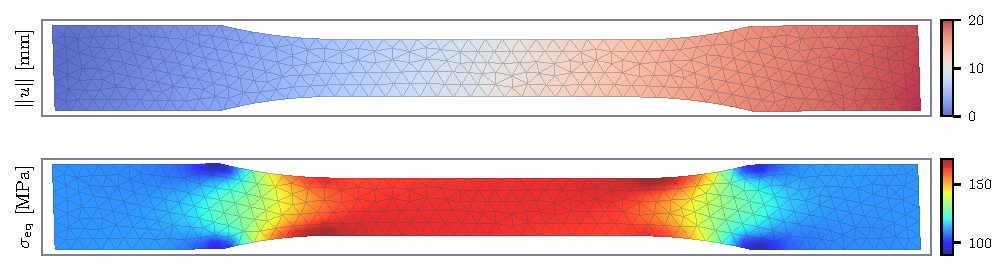
\includegraphics[width=.99\linewidth]{coupon_fields.pdf}
 \caption{Nested FOM--FE$^2$ reference at 100 kN per end, shown on the deformed mesh without displacement amplification.  Top: displacement magnitude.  Bottom: in-plane von Mises equivalent of the macroscopic Cauchy stress, $\sigma_{\rm eq}=(\sigma_{11}^2-\sigma_{11}\sigma_{22}+\sigma_{22}^2+3\sigma_{12}^2)^{1/2}$; Gauss-point values are averaged to the nodes for visualization.}
 \label{fig:coupon}
\end{figure}

\paragraph{Error and timing definitions.}
For a saved nodal or integration-point array $A$, the reported relative error is
\begin{equation}
 e_A=100\frac{\|\operatorname{vec}(A-A_0)\|_2}{\|\operatorname{vec}(A_0)\|_2},
 \label{eq:error}
\end{equation}
where $A_0$ is the nested reference on the same meshes. These are unweighted discrete array norms. The strain array stores engineering shear, whereas the stress array stores tensor shear. They are neither quadrature-weighted continuum $L^2$ norms nor invariant tensor Frobenius norms. The metric is kept identical across models; this does not make the three different field errors interchangeable.

Online wall time includes the complete macroscopic solve, microscopic or surrogate stress/tangent evaluations, communication, and lazy worker construction within the timed solve. Parent setup, offline data generation, training, reduced-mesh construction outside the timed region, and result export are excluded. The FOM uses 20 worker processes with one numerical-library thread per worker. The three optimized microscopic surrogates use the same process configuration and three sequential fresh complete runs. PANN evaluations are batched in one process, with the number of PyTorch threads selected by a preliminary sweep.

The macroscopic solve stops when the free-degree-of-freedom residual norm falls below $10^{-5}$ N or its ratio to the initial increment residual falls below $10^{-7}$. The periodic FOM uses a relative microscopic displacement-increment tolerance of $10^{-10}$, with continuation when needed. The FOM and PANN times come from single runs, so their ratios are observed online speed-ups under the stated implementations rather than matched-thread efficiency estimates.

The affine HPROM uses its exact reduced residual Jacobian, whereas HPROM--ANN uses the projected-stiffness modified-Newton matrix described in Section~\ref{sec:adaptive_weights}; both use a microscopic increment tolerance of $10^{-10}$. Their effective constitutive tangents nevertheless account for the equilibrium sensitivity of their respective full residuals. The reported speed-up compares these implemented workflows, including their different iteration matrices and derivative costs; it does not isolate a nonlinear-representation gain or quantify the iteration penalty of modified Newton.

\begin{table}[htbp]
 \centering\small
 \caption{Coupon simulations: final-field errors of Eq.~\eqref{eq:error} with respect to the nested FOM, online wall time, and speed-up over the FOM.}
 \label{tab:fe2}
 \begin{tabular}{lrrrrr}
\toprule
Model & $e_u$ [\%] & $e_E$ [\%] & $e_S$ [\%] & Time [s] & Speed-up \\
\midrule
FOM & -- & -- & -- & 4268.68 & -- \\
HPROM & 0.0057 & 0.0165 & 0.0010 & 67.35 & 63.38 \\
HPROM--ANN & 0.0520 & 0.1497 & 0.0373 & 30.14 & 141.61 \\
D-HPROM--ANN & 0.0232 & 0.0485 & 0.0097 & 3.79 & 1126.90 \\
ICNN & 0.4066 & 0.6785 & 0.0739 & 1.04 & 4105.14 \\
ICKAN & 0.4197 & 0.6914 & 0.0732 & 1.95 & 2187.66 \\
Unconstrained energy & 0.0022 & 0.0050 & 0.0006 & 1.48 & 2884.31 \\
\bottomrule
\end{tabular}

\end{table}

\paragraph{Accuracy--cost trade-off and Newton behavior.}
Table~\ref{tab:fe2} shows distinct operating points rather than a single universally best model. Among the reduced microscopic models, the linear HPROM gives the smallest displacement error, approximately $0.0057\%$, at a median online time of 67.35 s. The iterative HPROM--ANN reduces this time to 30.14 s with a displacement error of approximately $0.0520\%$. The iterative nonlinear model is therefore about $2.23$ times faster than the linear one, both in their optimized implementations. The direct closure reduces the time to 3.79 s and has a displacement error of approximately $0.0232\%$ on this path. Its lower error than the iterative nonlinear model is an observed outcome, not a consequence of a general error ordering.

The six-feature ICNN and ICKAN take 1.04 s and 1.95 s, with displacement errors of approximately $0.407\%$ and $0.420\%$, below their constitutive test errors but above those of the reduced microscopic models on this benchmark. The Unconstrained energy takes 1.48 s and gives the smallest displacement error in Table~\ref{tab:fe2}, $0.0022\%$, which mirrors the constitutive ordering of Section~\ref{sec:constitutive_accuracy}. Every saved coupon state lies inside the box, where all three energies have positive rank-one curvature at every sampled state, so this tensile path does not exercise the guarantees that separate them. On this path the constrained energies trade about two orders of magnitude in structural accuracy for admissibility beyond the data, while keeping the displacement error near $0.4\%$.

All models require four macroscopic iterations per increment, so this example provides no evidence that polyconvexity reduces Newton iterations. Inside the box, the constrained energies thus run in the common structural solver like the Unconstrained energy, at comparable cost. Their guarantees matter at states that the coupon never reaches, and the next example reaches them deliberately.

\subsubsection{Confined compression beyond the data}
\label{sec:confined}
Confined compression reaches such states through compaction.  A square block of side 10~mm, meshed with 128 quadratic triangles, is compressed by a uniform traction on one face while rigid, frictionless walls fix the normal displacement of the other three (Fig.~\ref{fig:confined}a).  The three SC-RVE energies, the assembly, and the Newton iteration are those of the coupon, and the load is applied in 20 equal increments up to 500~MPa, in $x$ or in $y$.  Compression in $x$ leaves the fitting box with the first increment, since the box contains no axial compression, and compression in $y$ leaves it beyond about $10\%$ shortening.  At every converged increment we also evaluate the rank-one curvature of Eq.~\eqref{eq:lh_background} at the 384 Gauss points of the block, minimized over unit directions.  Where it is positive, the incremental equilibrium problem is strongly elliptic.

\begin{figure}[t]
 \centering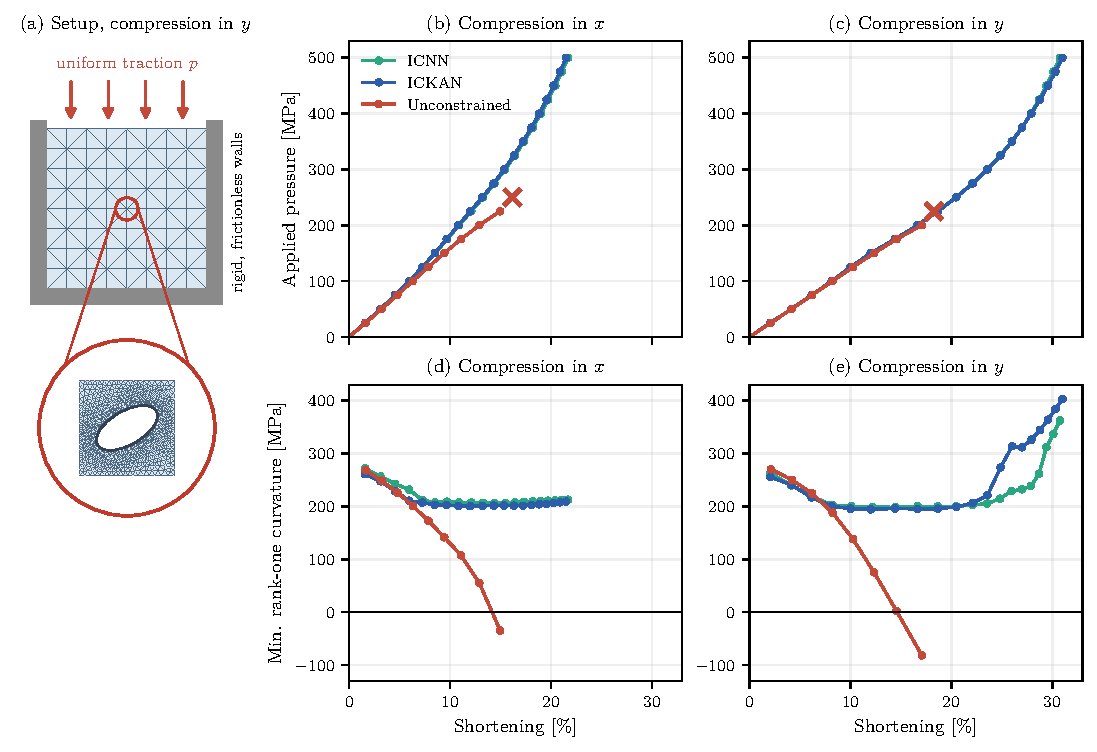
\includegraphics[width=.86\linewidth]{confined_compression.pdf}
 \caption{Confined compression beyond the data with the SC-RVE energies.  (a) Setup for compression in $y$: the homogenized block, meshed with 128 quadratic triangles, evaluates the SC-RVE energy at every integration point; for compression in $x$ the traction acts on a vertical face.  (b, c) Applied pressure versus shortening, one marker per increment of 25~MPa; a cross marks the increment in which Newton does not converge.  (d, e) Minimum rank-one curvature over the 384 Gauss points of the block at each converged increment.}
 \label{fig:confined}
\end{figure}

Both constrained energies reach 500~MPa in both directions, with four to nine Newton iterations per increment and final shortenings of about $22\%$ in $x$ and $31\%$ in $y$ (Fig.~\ref{fig:confined}b,c).  The Unconstrained energy follows a softer curve in $x$ and nearly the same curve in $y$, until Newton does not converge within 50 iterations in the increment to 250~MPa in $x$ and to 225~MPa in $y$.  This stop coincides with a loss of rank-one convexity in the block (Fig.~\ref{fig:confined}d,e).  The minimum curvature of the Unconstrained energy falls steadily with the load and turns negative at the last converged increment, at one of the 384 Gauss points in $x$ and at two in $y$.  These points lie in the elements at the corner where the left and bottom walls meet, where the local volume ratio has fallen to $J$ between 0.61 and 0.72.  The constrained energies, rank-one convex by construction, keep the minimum curvature above 194~MPa at every Gauss point and increment.  The test does not compare accuracy, because neither data nor a reference exist at these states; it shows which energies keep the structural problem solvable once it leaves the data.

\section{Conclusions}
\label{sec:conclusions}
Paired directional features with constrained trainable powers and determinant exponents provide a practical polyconvex constitutive construction for the anisotropic periodic cells studied here.  Their isotropic reference derivatives allow exact stress normalization through an affine determinant correction without tying the normalization coefficient to the volumetric barrier stiffness.  The proof combines feature convexity in independent minors with core convexity and monotonicity, and includes every correction in the complete energy.  Global nonnegative energy is supported separately by a sufficient bound evaluated for the saved parameters, which certifies every learned six-feature model of this study.

The two cells separate representation from deployment.  On the multicavity cell, learning six paired features reduces the held-out stress error sevenfold, to about $0.04\%$, and prescribing more directions does not close this gap.  On the single-cavity cell, the selected ICNN and ICKAN attain approximately $0.63\%$ held-out stress error and below $0.42\%$ displacement error in the coupon simulation.  The Unconstrained energy, trained under the same protocol, is more accurate inside the data by a factor of about six on the first cell and about 120 on the second, and controls of capacity and feature count attribute this price to the admissible construction rather than to network size.  Beyond the data, the Unconstrained energy loses rank-one convexity and remains finite under volume collapse, whereas the constrained energies are rank-one convex everywhere and grow without bound as the volume vanishes.

Optimized reduced microscopic models provide a complementary accuracy--cost reference.  They are more accurate than the constrained energies on the coupon, while direct learned constitutive evaluation is generally faster, and all compared models converge with the same number of macroscopic iterations per increment.  Because every coupon state lies inside the data, that example does not exercise the guarantees, and the Unconstrained energy is the most accurate model there.  Confined compression takes the same energies beyond the data.  The constrained energies then carry the block to 500~MPa in both directions, whereas with the Unconstrained energy Newton stops below half that load, exactly when its rank-one curvature turns negative at a corner of the block.  The accuracy given up is thus the price of a structural problem that remains solvable beyond the data, which is the property the construction is designed to secure.

\FloatBarrier
\appendix
\section{Rank-one paths and finite-strain energy curvature}
\label{app:finite_strain_curvature}
This appendix supplies the algebra behind the two finite-strain curvature statements in criterion (C5). For a twice differentiable energy, nonnegative curvature along every rank-one perturbation is expressed by the Legendre--Hadamard condition
\begin{equation}
 \partial^2_{\F\F}W(\F)[\bm a\otimes\bm b,\bm a\otimes\bm b]\geq0
 \quad\hbox{for all }\bm a,\bm b\in\R^2 .
 \label{eq:lh_background}
\end{equation}
The argument below shows why the polyconvex representation in Eq.~\eqref{eq:polyconvex_definition} implies this condition.

\paragraph{Determinant along a rank-one path.}
For arbitrary $\F,\bm H\in\R^{2\times2}$, expansion of the two products in the determinant gives
\begin{align}
 \det(\F+t\bm H)
 &=(F_{11}+tH_{11})(F_{22}+tH_{22})
 -(F_{12}+tH_{12})(F_{21}+tH_{21})\nonumber\\
 &=\det\F+t(F_{22}H_{11}+F_{11}H_{22}
 -F_{21}H_{12}-F_{12}H_{21})+t^2\det\bm H.
\end{align}
The coefficient of $t$ is $\cof\F:\bm H$, since
\begin{equation}
 \cof\F=\begin{pmatrix}F_{22}&-F_{21}\\-F_{12}&F_{11}\end{pmatrix},
 \qquad \bm A:\bm B=\sum_{i,j}A_{ij}B_{ij}.
\end{equation}
For $\bm H=\bm a\otimes\bm b$, its entries are $H_{ij}=a_i b_j$, so
\begin{equation}
 \det\bm H=a_1b_1a_2b_2-a_1b_2a_2b_1
 =a_1a_2(b_1b_2-b_2b_1)=0.
\end{equation}
The determinant is therefore affine along a rank-one path:
\begin{equation}
 \det(\F+t\bm a\otimes\bm b)
 =\det\F+t\,\cof\F:(\bm a\otimes\bm b).
 \label{eq:rankone_minor_line}
\end{equation}
If $\F_B=\F_A+\bm H$ and $\F_s=(1-s)\F_A+s\F_B$, with $\bm H=\bm a\otimes\bm b$, then
\begin{equation}
 (\F_s,\det\F_s)
 =(1-s)(\F_A,\det\F_A)+s(\F_B,\det\F_B).
\end{equation}
For $0\leq s\leq1$ and positive endpoint determinants, the whole segment remains admissible. Convexity of $\mathcal P$ therefore yields
\begin{equation}
 W(\F_s)\leq(1-s)W(\F_A)+sW(\F_B).
\end{equation}
For a twice differentiable energy, the restriction to this line consequently has nonnegative second derivative, as required by Eq.~\eqref{eq:lh_background}.

\paragraph{Strain curvature and the chain rule.}
Let $\bm H\in\R^{2\times2}$ be an arbitrary perturbation and let $t$ parametrize $\F(t)=\F+t\bm H$. Dots denote derivatives with respect to $t$, and $\operatorname{sym}(\bm A)=(\bm A+\bm A^T)/2$ denotes the symmetric part of a matrix. Direct multiplication gives
\begin{align}
 \E(t)
 &=\tfrac12\bigl[\F^T\F-\I
 +t(\F^T\bm H+\bm H^T\F)+t^2\bm H^T\bm H\bigr]\nonumber\\
 &=\E(0)+t\operatorname{sym}(\F^T\bm H)
 +\tfrac12t^2\bm H^T\bm H.
\end{align}
Thus $\dot\E(0)=\operatorname{sym}(\F^T\bm H)$ and $\ddot\E(0)=\bm H^T\bm H$. Using the engineering-strain convention of Eq.~\eqref{eq:voigt}, the chain and product rules give
\begin{align}
 \frac{\dd W}{\dd t}&=\ssv\cdot\dot\ee,\nonumber\\
 \frac{\dd^2 W}{\dd t^2}
 &=\sum_{i,j}\frac{\partial s_i}{\partial e_j}\dot e_j\dot e_i
 +\sum_i s_i\ddot e_i
 =\dot\ee^{\,T}\bm D\dot\ee+\Sg:\ddot\E.
\end{align}
Substituting $\ddot\E(0)$ gives
\begin{equation}
 \left.\frac{\dd^2 W(\F+t\bm H)}{\dd t^2}\right|_{t=0}
 =\dot{\ee}(0)^T\bm D\dot{\ee}(0)+\Sg:(\bm H^T\bm H).
 \label{eq:strain_vs_F_curvature}
\end{equation}
Here $\bm D=\partial\ssv/\partial\ee$ is the strain tangent and $\Sg$ is the second Piola--Kirchhoff stress, both evaluated at $t=0$. The first term accounts for the change of stress with strain; the second accounts for the curvature of the strain path, weighted by the current stress. Even if $\bm D$ is positive semidefinite, the stress term can be negative in compression.

\paragraph{An analytical counterexample.}
Consider $W(\E)=\mu\E:\E$, where $\mu>0$ is a constant with units of energy density. One has $\Sg=2\mu\E$. Since
\begin{equation}
 W(\ee)=\mu(e_1^2+e_2^2+e_3^2/2),
 \qquad \bm D=\diag(2\mu,2\mu,\mu),
\end{equation}
the energy is strictly convex in engineering strain. At $\F=\lambda\I$, where $\lambda>0$ is the common in-plane stretch, choose the rank-one perturbation $\bm H=\diag(1,0)$. Then
\begin{equation}
 \dot\ee=(\lambda,0,0)^T,\qquad
 \Sg=\mu(\lambda^2-1)\I,\qquad
 \bm H^T\bm H=\diag(1,0).
\end{equation}
Hence the strain-tangent term is $2\mu\lambda^2$, and the stress term is $\mu(\lambda^2-1)$, giving
\begin{equation}
 \left.\frac{\dd^2 W(\lambda\I+t\bm H)}{\dd t^2}\right|_{t=0}
 =2\mu\lambda^2+\mu(\lambda^2-1)
 =\mu(3\lambda^2-1).
 \label{eq:strain_convex_counterexample}
\end{equation}
At $\lambda=1/2$, the curvature is $-\mu/4$, violating Eq.~\eqref{eq:lh_background} despite convexity in $\E$. This is an analytical counterexample, not a sampled observation about the RVE or a trained model. Compression alone does not force negative curvature: at $\lambda=3/4$, the same expression is $11\mu/16>0$.

Equivalently, direct substitution gives
\begin{equation}
 W(\lambda\I+t\bm H)
 =\frac\mu4\bigl[(\lambda+t)^2-1\bigr]^2
 +\frac\mu4(\lambda^2-1)^2,
\end{equation}
whose second derivative at zero is $\mu(3\lambda^2-1)$. The path is admissible near zero because $\det(\lambda\I+t\bm H)=\lambda(\lambda+t)>0$ for $t>-\lambda$.

\section{Proofs for the paired features and complete energy}
\label{app:convex}
The proof follows the construction used in the main text. We first isolate one stretch--determinant contribution and derive the exponent bounds that make it convex. We then assemble two perpendicular contributions and compute their reference derivative, proving Proposition~\ref{prop:paired_features}. Finally, we compose the resulting features with the monotone convex core and examine $W_{\rm learn}$, $W_{\rm corr}$, $W_{\rm vol}$, and $W_{\rm dist}$ to establish Proposition~\ref{prop:complete_energy}.

\subsection{Joint convexity of the directional building block}
Every contribution in Eq.~\eqref{eq:features} has the form
\begin{equation}
 f(\bm x,J)=\|\bm x\|^aJ^{-b},
 \qquad \bm x=\F\bm d,
\end{equation}
up to a positive constant, with $a=2p$ or $2q$. It is therefore enough to determine when this building block is jointly convex in $(\bm x,J)$. Let $t=\|\bm x\|>0$. Because $f$ depends on $\bm x$ only through $t$, its Hessian separates into a block coupling the radial variable $t$ to $J$ and transverse directions orthogonal to $\bm x$. The radial--determinant block is
\begin{equation}
 \begin{pmatrix}
 a(a-1)t^{a-2}J^{-b} & -ab t^{a-1}J^{-b-1}\\
 -ab t^{a-1}J^{-b-1} & b(b+1)t^aJ^{-b-2}
 \end{pmatrix}.
\end{equation}
For this symmetric $2\times2$ block to be positive semidefinite, its diagonal entries and determinant must be nonnegative. The diagonal entries are nonnegative for $a\geq1$ and $b\geq0$, while the determinant is
\begin{align}
 \det &=ab\bigl[(a-1)(b+1)-ab\bigr]t^{2a-2}J^{-2b-2}\nonumber\\
 &=ab(a-b-1)t^{2a-2}J^{-2b-2}\geq0.
\end{align}
The factor $a-b-1$ gives the upper bound $b\leq a-1$; if this bound is violated, the determinant is negative and the block has curvatures of opposite sign. The remaining, transverse Hessian eigenvalues are $a t^{a-2}J^{-b}\geq0$. Hence $a\geq1$ and $0\leq b\leq a-1$ make the complete Hessian positive semidefinite. Continuous extension gives convexity at $\bm x=0$. For the constitutive evaluation on $\GL$, a nonzero reference direction cannot satisfy $\F\bm d=0$, so this point does not introduce an interior singularity of the directional norm. Substituting $a=2p$ gives $p\geq\tfrac12$ and $0\leq b\leq2p-1$; the same argument with $(q,c)$ establishes all bounds in Eq.~\eqref{eq:featureconstraints}.

\subsection{Proof of Proposition~\ref{prop:paired_features}}
\begin{proof}
\emph{Convexity and objectivity.}
For any fixed learned parameter set, the directions $\bm d_i$ and $\bm d_i^\perp$ are independent of deformation. The maps $\F\mapsto\F\bm d_i$ and $\F\mapsto\F\bm d_i^\perp$ are therefore linear. Composing the convex building block above with these maps, multiplying by the positive factors $1/p_i$ and $1/q_i$, and adding the two contributions proves convexity of $z_i$ in independent $(\F,J)$. A left proper rotation changes $\F\bm d$ to $\bm Q\F\bm d$ without changing its norm, so each contribution is objective.

\emph{Reference value and derivative.}
We now return to the physical relation $J=\det\F$, still holding every learned parameter fixed. At $\E=\bm0$, both directional invariants and $J$ equal one, so the two contributions give $z_i^0=1/p_i+1/q_i$. Moreover, $I_4(\bm d_i)=\bm d_i^T(\I+2\E)\bm d_i$ and $J^2=(1+2E_{11})(1+2E_{22})-4E_{12}^2$ imply $\partial_{\E}I_4(\bm d_i)=2\bm d_i\otimes\bm d_i$ and $\partial_{\E}J|_0=\I$. Applying the product rule to the first contribution gives
\begin{equation}
 \left.\partial_{\E}\frac{I_4(\bm d_i)^{p_i}}{p_iJ^{b_i}}\right|_0
 =\frac1{p_i}\bigl[2p_i\bm d_i\otimes\bm d_i-b_i\I\bigr]
 =2\bm d_i\otimes\bm d_i-\frac{b_i}{p_i}\I.
\end{equation}
The prefactor $1/p_i$ has cancelled the factor $p_i$ produced by differentiating the stretch power. The perpendicular contribution has the same form with $(\bm d_i,p_i,b_i)$ replaced by $(\bm d_i^\perp,q_i,c_i)$. The two directional projectors satisfy $\bm d_i\otimes\bm d_i+\bm d_i^\perp\otimes\bm d_i^\perp=\I$; adding the contributions therefore removes the directional dependence at the reference and gives
\begin{equation}
 \left.\partial_{\E}z_i\right|_0
 =2(\bm d_i\otimes\bm d_i+\bm d_i^\perp\otimes\bm d_i^\perp)
 -\left(\frac{b_i}{p_i}+\frac{c_i}{q_i}\right)\I
 =\rho_i\I.
\end{equation}
In the work-conjugate engineering-strain convention of Eq.~\eqref{eq:voigt}, this tensor gradient corresponds to $\partial_{\ee}z_i|_0=\rho_i(1,1,0)^T$, proving Eq.~\eqref{eq:referencefeatures}.
\end{proof}

\paragraph{Positive affine conditioning.}
The raw feature is converted to the core input by $y_i=(z_i-z_i^{\rm cen})/s_i$, with $s_i>0$ independent of deformation. Writing $\bm X=(\F,J)$,
\begin{equation}
 \partial^2_{\bm X\bm X}y_i=\frac1{s_i}\partial^2_{\bm X\bm X}z_i,
 \qquad
 y_i(\bm X_B)-y_i(\bm X_A)
 =\frac{z_i(\bm X_B)-z_i(\bm X_A)}{s_i}.
\end{equation}
The first identity preserves positive-semidefinite curvature and the second preserves componentwise order. Thus the numerical conditioning applied before the monotone core changes neither property used in the composition proof below.

\subsection{Proof of Proposition~\ref{prop:complete_energy}}
\label{app:complete_energy_proof}

\begin{proof}
\emph{Potential structure, objectivity, and stress symmetry (C1)--(C3).}
Every directional norm and $J$ is unchanged by left proper rotations. The features can also be expressed through $\bm d_i^T\C\bm d_i$ and $\sqrt{\det\C}$. Hence the complete energy is objective, and differentiation with respect to symmetric strain gives a symmetric material stress. Differentiating this scalar energy supplies (C1) and the major symmetry of its strain tangent. Smoothness holds on $\GL$ because $J>0$, nonzero material directions have nonzero deformed length, and both cores are $C^2$. Because this argument uses left rotations only, it does not impose a material symmetry group.

\emph{Reference normalization (C4).}
Equation~\eqref{eq:energy_reference_value} shows that $W_{\rm learn}$ sets the reference energy, and Eq.~\eqref{eq:energy_reference_stress} shows that $W_{\rm corr}$ cancels the learned reference stress. The calculations for $W_{\rm vol}$ and $W_{\rm dist}$ in Section~\ref{sec:energy_admissibility} show that both growth terms have zero value and zero strain gradient at the reference. Thus the complete energy satisfies both reference conditions.

\emph{Polyconvexity (C5).} Let $\bm G\in\R^{2\times2}$ and $j>0$ be independent. Define $\mathcal P(\bm G,j)$ by the right-hand side of Eq.~\eqref{eq:energy}, replacing $\bm z$ by $\bm z(\bm G,j)$, $J$ by $j$, and $\tr\C$ by $\|\bm G\|_F^2$. For two such pairs $\bm X_1=(\bm G_1,j_1)$, $\bm X_2=(\bm G_2,j_2)$ and $0\leq t\leq1$,
\begin{align}
 H\!\left(\bm z(t\bm X_1+(1-t)\bm X_2)\right)
 &\leq H\!\left(t\bm z(\bm X_1)+(1-t)\bm z(\bm X_2)\right)\nonumber\\
 &\leq tH(\bm z(\bm X_1))+(1-t)H(\bm z(\bm X_2)).
 \label{eq:convex_composition_proof}
\end{align}
The first inequality uses feature convexity and core monotonicity; the second uses core convexity. Therefore $W_{\rm learn}$ is convex up to its constant reference subtraction. The correction $W_{\rm corr}=-r(j-1)$ is affine for either sign of $r$, while $W_{\rm vol}$ and $W_{\rm dist}$ are convex in independent $(\bm G,j)$ because their nonaffine parts are positive multiples of $-\log j$, $(j-1)^2$, and $\|\bm G\|_F^2$. Thus $\mathcal P$ is convex and $W(\F)=\mathcal P(\F,\det\F)$, establishing Eq.~\eqref{eq:polyconvex_definition}.

\emph{Growth (C6).}
Convexity of $H$ gives its supporting-plane inequality at $\bm z^0$:
\begin{equation}
 H(\bm z)\geq H(\bm z^0)+\sum_i h_i(z_i-z_i^0)
 \geq H(\bm z^0)-\sum_i h_i z_i^0.
\end{equation}
The second inequality uses $h_i,z_i\geq0$. Hence $W_{\rm learn}$ has a deformation-independent lower bound and cannot cancel the analytic growth terms. As $J\to0^+$, the logarithmic part of $W_{\rm vol}+W_{\rm dist}$ diverges while $W_{\rm corr}$ remains bounded. As $J\to\infty$, the positive quadratic part of $W_{\rm vol}$ dominates every potentially negative linear or logarithmic term. Finally, if $J$ remains in a compact subset of $(0,\infty)$ while $\|\F\|_F\to\infty$, the term $\varepsilon\|\F\|_F^2/2$ in $W_{\rm dist}$ diverges and all determinant-only terms remain bounded. These are the three stated growth limits.
\end{proof}

\section{Sufficient lower bound for nonnegative energy}
\label{app:nonnegative}
Define $k_i=1/p_i+1/q_i$ and $\eta_i=\rho_i/k_i$. Write $t=\|\F\bm d_i\|^2$, $u=\|\F\bm d_i^\perp\|^2$. Hadamard's determinant inequality gives $tu\geq J^2$. Since each feature is increasing in $t,u$, its minimum at fixed $J$ occurs on $tu=J^2$. Minimizing
\begin{equation}
 \frac{t^{p_i}}{p_iJ^{b_i}}+\frac{J^{2q_i-c_i}t^{-q_i}}{q_i}
\end{equation}
gives $t^{p_i+q_i}=J^{2q_i+b_i-c_i}$ and hence $z_i\geq k_iJ^{\eta_i}$. This is a separate lower bound for each feature; simultaneous attainability for all directions is not assumed. It therefore remains valid after summing the supporting-plane inequalities.

Together with $\tr\C/2\geq J$ and the supporting plane of $H$, this feature bound gives
\begin{equation}
 W\geq g(J):=\sum_i h_i k_i[J^{\eta_i}-1-\eta_i(J-1)]
 +(\alpha+\varepsilon)(J-1-\log J)+\frac\beta2(J-1)^2.
 \label{eq:lowerbound}
\end{equation}
Because $g(1)=g'(1)=0$, it remains to establish $g''(J)\geq0$ for every $J>0$. Differentiation gives
\begin{equation}
 J^2g''(J)=\alpha+\varepsilon+\beta J^2+\sum_i c_i^*J^{\eta_i},
 \qquad c_i^*=h_i k_i\eta_i(\eta_i-1).
\end{equation}
Only terms with $0<\eta_i<1$ can have negative coefficients. If $c_-=\sum_{c_i^*<0}|c_i^*|$, the two inequalities
\begin{align}
 \alpha+\varepsilon+\sum_{\eta_i<0}c_i^*-c_-&\geq0,\\
 \beta+\sum_{\eta_i\geq1}c_i^*-c_-&\geq0
\end{align}
are sufficient on $0<J\leq1$ and $J\geq1$, respectively. For the first region, $J^{\eta_i}\leq1$ for negative-coefficient terms and $J^{\eta_i}\geq1$ when $\eta_i<0$. For the second region, divide $J^2g''$ by $J$: all negative-coefficient powers then satisfy $J^{\eta_i-1}\leq1$, while $J^{\eta_i-1}\geq1$ for $\eta_i\geq1$ and $\beta J\geq\beta$. Dropping the remaining nonnegative contributions gives the stated bounds. Their failure is inconclusive.

The selected parameters require a sharper check. The audit partitions $[10^{-4},10^4]$ into 4000 logarithmically spaced intervals. On each interval $[J_L,J_R]$, a positive power term is bounded below by the smaller endpoint value, whereas a negative-coefficient term is bounded below by $c_i^*J_R^{\eta_i}$, since its exponent lies in $(0,1)$. The constant and quadratic terms are bounded below by $\alpha+\varepsilon$ and $\beta J_L^2$. Below the finite interval, the nonnegative negative-exponent terms increase and the magnitudes of the negative-coefficient terms decrease toward $J=0$. Above it, factoring out $J^{\eta_-}$ with $\eta_-=\max_{c_i^*<0}\eta_i<1$ yields a lower bound whose retained positive powers increase. These endpoint and tail inequalities cover every $J>0$, not only the grid points. Positive margins establish the sufficient analytical argument for the saved parameters to the accuracy of its floating-point evaluation; random energy samples alone would not establish it.

\section{Latent-space closure details}
\label{app:latent_closure}
This appendix supplies the algebra omitted from Section~\ref{sec:latent_closure}. Let $\bm\Phi\in\R^{N\times n_{\rm tot}}$ be the retained orthonormal POD basis, let $\bm S_{\rm snap}$ collect the centered displacement snapshots, and collect the corresponding engineering-strain inputs in $\bm M=[\,\ee^1,\ldots,\ee^{N_s}\,]$. Their POD coefficients are
\begin{equation}
 \bm Q_{\rm POD}=\bm\Phi^T\bm S_{\rm snap}.
\end{equation}
The input-informed construction first identifies the least-squares map from these coefficients to strain,
\begin{equation}
 \bm T_m=\bm M\bm Q_{\rm POD}^{\dagger}
 \in\arg\min_{\bm H}\|\bm H\bm Q_{\rm POD}-\bm M\|_F^2,
\end{equation}
where $\dagger$ denotes the Moore--Penrose pseudoinverse. Assuming rank three, the compact factorization
\begin{equation}
 \bm\Phi\bm T_m^T=\bm V\bm\Sigma_m\bm Z_m^T,
 \qquad
 \bm A_m=\bm\Sigma_m^{-1}\bm Z_m^T
\end{equation}
defines the three-column orthonormal primary block $\bm V$ and its coordinate scaling $\bm A_m$. The secondary block $\overline{\bm V}$ is an orthonormal complement within the retained POD span, ordered by snapshot energy. With $\bm q=\bm A_m\bm\xi$, the deployed decoder is
\begin{equation}
 \widetilde{\bm u}(\bm\xi)=\bm u_{\rm ref}
 +\bm V\bm A_m\bm\xi
 +\overline{\bm V}\widehat{\mathcal N}(\bm\xi),
 \qquad
 \bm\xi^s=\bm T_m\bm Q_{\rm POD}^{\,s}.
\end{equation}
Thus $\bm\xi^s\approx\ee^s$ is a fitted snapshot relation, not a kinematic identity.

The displacement error separates the two approximation mechanisms. For $\bm V_{\rm tot}=[\,\bm V,\overline{\bm V}\,]$ and projected coordinates $(\bm q^s,\overline{\bm q}^{\,s})$,
\begin{equation}
 \|\bm u^s-\widetilde{\bm u}(\bm q^s)\|_2^2
 =\|\overline{\bm q}^{\,s}-\mathcal N(\bm q^s)\|_2^2
 +\|(\bm I-\bm V_{\rm tot}\bm V_{\rm tot}^T)
       (\bm u^s-\bm u_{\rm ref})\|_2^2.
\end{equation}
The first term is the closure error within the retained span; the second is the POD truncation error. Increasing network capacity cannot recover a displacement component excluded from $\bm V_{\rm tot}$.

Finally, let $\bm B_{\xi}=\partial_{\bm\xi}\widetilde{\bm u}$, $\bm R$ be the constrained microscopic residual, and $\bm K=\partial_{\bm u}\bm R$. Differentiating the projected residual $\bm r=\bm B_{\xi}^T\bm R$ gives
\begin{equation}
 \frac{\partial\bm r}{\partial\bm\xi}
 =\bm B_{\xi}^T\bm K\bm B_{\xi}
 +\sum_{j=1}^{N}R_j
   \frac{\partial^2\widetilde u_j}
        {\partial\bm\xi\,\partial\bm\xi}.
\end{equation}
The second term is the curvature contribution of the decoder manifold. It need not vanish at reduced equilibrium because $\bm B_{\xi}^T\bm R=\bm0$ does not imply $\bm R=\bm0$.

\section{Elementwise cubature conventions}
\label{app:cubature}
This appendix records the implementation conventions omitted from Section~\ref{sec:reduced}. The general ECM construction and MAW--ECM pruning algorithm follow Refs.~\cite{hernandez2017,hernandez2026dimensional}; the expressions below specify how the deployed residual and stress rules are assembled.

\paragraph{Fixed rule.}
Let $\bm c_e^s\in\R^d$ contain the contribution of element $e$ at training state $s$. Residual cubature uses $\bm c_e^s=\bm h_e^s$. Stress cubature uses the four components of
\begin{equation}
 \bm p_e^s=\frac{1}{|Y|}\sum_{g\in e}\omega_g\bm P_{\mu,g}^s,
 \qquad
 \bm c_e^s=\operatorname{vec}\bm p_e^s
 =\begin{bmatrix}p_{e,11}^s&p_{e,12}^s&p_{e,21}^s&p_{e,22}^s\end{bmatrix}^{T}.
\end{equation}
One element occupies each row of the sampled integrand matrix,
\begin{equation}
 \bm M_{\rm int}=
 \begin{bmatrix}
  (\bm c_1^1)^T&\cdots&(\bm c_1^{N_c})^T\\
  \vdots&&\vdots\\
  (\bm c_{N_{\rm el}}^1)^T&\cdots&(\bm c_{N_{\rm el}}^{N_c})^T
 \end{bmatrix}
 \in\R^{N_{\rm el}\times(dN_c)}.
\end{equation}
A truncated SVD gives $\bm M_{\rm int}\simeq\bm U_{\rm cub}\bm\Sigma_{\rm cub}\bm V_{\rm cub}^T$. To enforce the multiplier sum without duplicating a constant component already represented by the retained integration modes, the fitting system uses
\begin{equation}
 \bm p_\perp=(\bm I-\bm U_{\rm cub}\bm U_{\rm cub}^T)\bm1,
 \qquad
 \bm G_{\rm cub}=
 \begin{bmatrix}
  \bm U_{\rm cub}^T\\
  \bm p_\perp^T/\|\bm p_\perp\|_2
 \end{bmatrix},
 \qquad
 \bm b_{\rm cub}=\bm G_{\rm cub}\bm1.
\end{equation}
If the constant already lies in the retained span, the last row is redundant. Otherwise its exact reproduction gives $\sum_e w_e=N_{\rm el}$. The reference quadrature measures are already contained in $\bm c_e^s$; the unknowns are element multipliers.

\paragraph{Adaptive neural fields.}
After MAW--ECM pruning selects a support $\mathcal Z=\{e_1,\ldots,e_m\}$, neural fitting returns to the uncompressed contributions at each decoded state:
\begin{equation}
 \bm A^s=
 \begin{bmatrix}
  \bm c_{e_1}^s&\cdots&\bm c_{e_m}^s\\
  1&\cdots&1
 \end{bmatrix},
 \qquad
 \bm b^s=
 \begin{bmatrix}
  \displaystyle\sum_{e\in\mathcal E}\bm c_e^s\\
  N_{\rm el}
 \end{bmatrix}.
 \label{eq:statewise_cubature_appendix}
\end{equation}
Thus the target uses the full-mesh sum, not the selected-column sum. Residual fitting uses $d=n$ and $\mathcal Z_r$; stress fitting uses $d=4$ and $\mathcal Z_s$. With the scaled-softmax map of Eq.~\eqref{eq:softmax_weights}, the residual network minimizes
\begin{equation}
 \mathcal L_{\rm cub}(\bm\theta_r)=
 \frac{1}{|\mathcal I_{\rm fit}|}
 \sum_{s\in\mathcal I_{\rm fit}}
 \frac{\|\bm A^s\bm w(\bm\xi^s)-\bm b^s\|_2^2}
      {\max(\|\bm b^s\|_2^2,\delta_{\rm floor})},
\end{equation}
and the stress network uses the analogous loss with $\bm v$. A preliminary fit to the sampled MAW--ECM weights initializes each network, but the final objective is integration accuracy; a reproducing weight vector is not unique.

\paragraph{Tangent evaluation.}
Both reduced implementations use Eq.~\eqref{eq:reduced_ift}, but evaluate its partial derivatives differently. For the affine HPROM, the assembled reduced stiffness and the analytic lifting derivative provide $\dd\qq_{\rm tra}^*/\dd\ee$ through three linear right-hand sides; central differences are applied only to the stress along those linearized equilibrium directions. For HPROM--ANN, central differences at fixed $\qq$ or fixed $\ee$ evaluate all four partial-derivative blocks in Eq.~\eqref{eq:reduced_ift}, including decoder curvature and weight variation. The resulting small linear system does not require a new nonlinear microscopic solve for every perturbed strain. Numerical differentiation is an implementation choice; analytic or automatic differentiation would give the same formal tangent subject to their respective numerical tolerances.

\section{Capacity and feature-count controls}
\label{app:capacity}
The comparisons of Section~\ref{sec:cell} pair compact constrained cores with a larger Unconstrained network.  To separate the effect of the constraints from that of capacity, both benchmarks complete a two-by-two design.  The constrained cores are widened to about 25\,000 parameters, comparable with the Unconstrained energy, and an Unconstrained energy with 981 parameters matches the compact ICNN.  Every new fit follows the protocol of Section~\ref{sec:training_protocol} with the same three seeds, and its test states are opened only once, after training has ended.

Table~\ref{tab:capacity_mc} reports the MC-RVE cells as medians over three seeds, as in Table~\ref{tab:mc_rve_m06}.  Widening changes the ICNN error from $0.0445\%$ to $0.0398\%$, while the Unconstrained energy improves from $0.0126\%$ to $0.0073\%$.  At matched capacity the constraints therefore cost a factor of 3.2 to 5.5 in stress error.  The wide ICKAN is less accurate than the compact one because two of its three seeds met the validation-plateau criterion early, so its row reflects the common stopping rule rather than capacity.

Table~\ref{tab:capacity_sc} reports the SC-RVE cells for the validation-selected seed, as in Table~\ref{tab:constitutive}, together with the coupon of Section~\ref{sec:coupon}.  Widening changes the constrained test errors by less than $3\%$, and the Unconstrained energy with 981 parameters remains about 75 to 80 times more accurate than either wide core.  In the coupon, the corresponding factor between matched cells lies between about 115 and 200.  Thirty-two learned features, trained with the same protocol, lower the test errors to $0.537\%$ and $0.618\%$ and the coupon errors to $0.343\%$ and $0.347\%$.  They also raise the probe errors to $35.6\%$ and $16.9\%$ (Section~\ref{sec:constitutive_accuracy}), and the sufficient bound of Appendix~\ref{app:nonnegative} fails for both saved parameter sets.  The six-feature models therefore remain the deployed choice.

\begin{table}[htbp]
 \centering\small
 \caption{MC-RVE capacity controls: independent-test errors, in percent.}
 \label{tab:capacity_mc}
 \begin{tabular}{lrrrr}
\toprule
Model & Parameters & Stress [\%] & Energy [\%] & Tangent [\%] \\
\midrule
ICNN, $m=6$ & 975 & 0.0445 & 0.0079 & 0.3851 \\
ICNN, wide & 26\,919 & 0.0398 & 0.0069 & 0.2962 \\
ICKAN, $m=6$ & 1\,659 & 0.0406 & 0.0066 & 0.3622 \\
ICKAN, wide$^\ast$ & 24\,847 & 0.0744 & 0.0104 & 1.8311 \\
Unconstrained, small & 981 & 0.0126 & 0.0019 & 0.1579 \\
Unconstrained & 25\,473 & 0.0073 & 0.0011 & 0.0857 \\
\bottomrule
\end{tabular}

\par\smallskip{\footnotesize Relative error norm over the 512 test states, median over three seeds. $^\ast$Adam stopped at the validation plateau after 28\,540 and 33\,330 steps for two of the three seeds, against 114\,910 for the third.}

\end{table}

\begin{table}[htbp]
 \centering\small
 \caption{SC-RVE capacity and feature-count controls, in percent.}
 \label{tab:capacity_sc}
 \begin{tabular}{lrrr}
\toprule
Model & Parameters & $e_S^{\rm test}$ [\%] & $e_u$ [\%] \\
\midrule
ICNN, $m=6$ & 975 & 0.6214 & 0.4066 \\
ICNN, wide & 26\,919 & 0.6066 & 0.4162 \\
ICNN, $m=32$ & 2\,379 & 0.5370 & 0.3433 \\
ICKAN, $m=6$ & 1\,659 & 0.6359 & 0.4197 \\
ICKAN, wide & 24\,847 & 0.6540 & 0.4322 \\
ICKAN, $m=32$ & 3\,999 & 0.6177 & 0.3469 \\
Unconstrained, small & 981 & 0.0081 & 0.0035 \\
Unconstrained & 25\,473 & 0.0052 & 0.0022 \\
\bottomrule
\end{tabular}

\par\smallskip{\footnotesize Validation-selected seed of each cell. Test: 400 states; $e_u$: final nodal displacement error of the coupon of Section~\ref{sec:coupon}.}

\end{table}

\begin{thebibliography}{99}

\bibitem{Miehe1999}
C. Miehe, J. Schr\"oder, J. Schotte, Computational homogenization
analysis in finite plasticity simulation of texture development in
polycrystalline materials, Computer Methods in Applied Mechanics
and Engineering 171(3--4) (1999) 387--418.
\doi{10.1016/S0045-7825(98)00218-7}

\bibitem{kouznetsova2001approach}
V.~G. Kouznetsova, W.~A.~M. Brekelmans, F.~P.~T. Baaijens,
An approach to micro--macro modeling of heterogeneous materials,
Computational Mechanics 27(1) (2001) 37--48.
\doi{10.1007/s004660000212}

\bibitem{geers2010multi}
M.~G.~D. Geers, V.~G. Kouznetsova, W.~A.~M. Brekelmans,
Multi-scale computational homogenization: Trends and challenges,
Journal of Computational and Applied Mathematics 234(7) (2010) 2175--2182.
\doi{10.1016/j.cam.2009.08.077}

\bibitem{feyel2003multilevel}
F. Feyel, A multilevel finite element method (FE$^2$) to describe the
response of highly non-linear structures using generalized continua,
Computer Methods in Applied Mechanics and Engineering 192(28--30) (2003)
3233--3244.
\doi{10.1016/S0045-7825(03)00348-7}

\bibitem{le2015computational}
B.~A. Le, J. Yvonnet, Q.-C. He, Computational homogenization of nonlinear
elastic materials using neural networks, International Journal for Numerical
Methods in Engineering 104(12) (2015) 1061--1084.
\doi{10.1002/nme.4953}

\bibitem{benner2015survey}
P. Benner, S. Gugercin, K.~E. Willcox, A survey of projection-based model
reduction methods for parametric dynamical systems, SIAM Review 57(4) (2015)
483--531.
\doi{10.1137/130932715}

\bibitem{yvonnet2007}
J. Yvonnet, Q.-C. He, The reduced model multiscale method (R3M) for the non-linear homogenization of hyperelastic media at finite strains, Journal of Computational Physics 223 (2007) 341--368. \doi{10.1016/j.jcp.2006.09.019}

\bibitem{Hernandez2014}
J.~A. Hern\'andez, J. Oliver, A.~E. Huespe, M.~A. Caicedo, J.~C.
Cante, High-performance model reduction techniques in computational
multiscale homogenization, Computer Methods in Applied Mechanics
and Engineering 276 (2014) 149--189.

\bibitem{hernandez2017}
J.A. Hern\'andez, M.A. Caicedo, A. Ferrer, Dimensional hyper-reduction of nonlinear finite element models via empirical cubature, Computer Methods in Applied Mechanics and Engineering 313 (2017) 687--722. \doi{10.1016/j.cma.2016.10.022}

\bibitem{Aldakheel2023}
F. Aldakheel, E.~S. Elsayed, T.~I. Zohdi, P. Wriggers, Efficient
multiscale modeling of heterogeneous materials using deep neural
networks, Computational Mechanics 72(1) (2023) 155--171.

\bibitem{kalina2023}
K.A. Kalina, L. Linden, J. Brummund, M. K\"astner, FEANN: an efficient data-driven multiscale approach based on physics-constrained neural networks and automated data mining, Computational Mechanics 71 (2023) 827--851. \doi{10.1007/s00466-022-02260-0}

\bibitem{Liu2022}
B. Liu, N. Kovachki, Z. Li, K. Azizzadenesheli, A. Anandkumar, A.~M.
Stuart, K. Bhattacharya, A learning-based multiscale method and its
application to inelastic impact problems, Journal of the
Mechanics and Physics of Solids 158 (2022) 104668.

\bibitem{Ghaderi2020}
A. Ghaderi, V. Morovati, R. Dargazany, A physics-informed assembly of
feed-forward neural network engines to predict inelasticity in
cross-linked polymers, Polymers 12(11) (2020) 2628.
\doi{10.3390/polym12112628}

\bibitem{AsadFarhat2026}
F. As'ad, C. Farhat, A staggered training framework for
mechanics-informed neural networks in tractable multiscale
homogenization with application to woven fabrics, Computer
Methods in Applied Mechanics and Engineering 452 (2026) 118666.

\bibitem{asad2022}
F. As'ad, P. Avery, C. Farhat, A mechanics-informed artificial neural network approach in data-driven constitutive modeling, International Journal for Numerical Methods in Engineering 123 (2022) 2738--2759. \doi{10.1002/nme.6957}

\bibitem{klein2022}
D.K. Klein, M. Fern\'andez, R.J. Martin, P. Neff, O. Weeger, Polyconvex anisotropic hyperelasticity with neural networks, Journal of the Mechanics and Physics of Solids 159 (2022) 104703. \doi{10.1016/j.jmps.2021.104703}

\bibitem{linden2023}
L. Linden, D.K. Klein, K.A. Kalina, J. Brummund, O. Weeger, M. K\"astner,
Neural networks meet hyperelasticity: A guide to enforcing physics,
Journal of the Mechanics and Physics of Solids 179 (2023) 105363.
\doi{10.1016/j.jmps.2023.105363}
Consulted full text: arXiv:2302.02403v2.

\bibitem{GaoNeffRoventaThiel2017}
D.~Y. Gao, P. Neff, I. Roventa, C. Thiel, On the convexity of
nonlinear elastic energies in the right Cauchy--Green tensor,
Journal of Elasticity 127 (2017) 303--308.
\doi{10.1007/s10659-016-9601-6}

\bibitem{Xu2021}
K. Xu, D.~Z. Huang, E. Darve, Learning constitutive relations using
symmetric positive definite neural networks,
Journal of Computational Physics 428 (2021) 110072.
\doi{10.1016/j.jcp.2020.110072}

\bibitem{ball1977}
J.M. Ball, Convexity conditions and existence theorems in nonlinear elasticity, Archive for Rational Mechanics and Analysis 63 (1977) 337--403.

\bibitem{Ciarlet1988}
P.~G. Ciarlet, Mathematical Elasticity, Volume I: Three-Dimensional
Elasticity, North-Holland, 1988.

\bibitem{SchroderNeff2003}
J. Schr\"oder, P. Neff, Invariant formulation of hyperelastic
transverse isotropy based on polyconvex free energy functions,
International Journal of Solids and Structures 40(2) (2003) 401--445.

\bibitem{Gasser2006}
T.~C. Gasser, R.~W. Ogden, G.~A. Holzapfel, Hyperelastic modelling of
arterial layers with distributed collagen fibre orientations,
Journal of the Royal Society Interface 3(6) (2006) 15--35.
\doi{10.1098/rsif.2005.0073}

\bibitem{amos2017}
B. Amos, L. Xu, J.Z. Kolter, Input convex neural networks, Proceedings of Machine Learning Research 70 (2017) 146--155. \url{https://proceedings.mlr.press/v70/amos17b.html}

\bibitem{Kalina2024}
K.A. Kalina, J. Brummund, W. Sun, M. K\"astner,
Neural networks meet anisotropic hyperelasticity: A framework based on generalized structure tensors and isotropic tensor functions,
Computer Methods in Applied Mechanics and Engineering 437 (2025) 117725.
\doi{10.1016/j.cma.2024.117725}
Consulted local version: arXiv:2410.03378v1 (2024).

\bibitem{klein2026}
D.K. Klein, K.A. Kalina, R. Ortigosa, J. Mart\'inez-Frutos, M. K\"astner, O. Weeger, Advances in polyconvex anisotropic hyperelasticity, arXiv:2605.27011v1 (2026). \url{https://arxiv.org/abs/2605.27011}

\bibitem{Linka2023}
K. Linka, E. Kuhl, A new family of Constitutive Artificial Neural
Networks towards automated model discovery,
Computer Methods in Applied Mechanics and Engineering 403 (2023) 115731.

\bibitem{Tac2022}
V. Tac, F. Sahli Costabal, A. Buganza Tepole, Data-driven tissue
mechanics with polyconvex neural ordinary differential equations,
Computer Methods in Applied Mechanics and Engineering 398 (2022) 115248.
\doi{10.1016/j.cma.2022.115248}

\bibitem{Abdolazizi2025}
K.P. Abdolazizi, R.C. Aydin, C.J. Cyron, K. Linka,
Constitutive Kolmogorov--Arnold networks (CKANs): Combining accuracy and interpretability in data-driven material modeling,
Journal of the Mechanics and Physics of Solids 203 (2025) 106212.
\doi{10.1016/j.jmps.2025.106212}

\bibitem{thakolkaran2025}
P. Thakolkaran, Y. Guo, S. Saini, M. Peirlinck, B. Alheit, S. Kumar, Can KAN CANs? Input-convex Kolmogorov-Arnold Networks (KANs) as hyperelastic constitutive artificial neural networks (CANs), Computer Methods in Applied Mechanics and Engineering 443 (2025) 118089. \doi{10.1016/j.cma.2025.118089}

\bibitem{Hernandez2020}
J.~A. Hern\'andez, A multiscale method for periodic structures using
domain decomposition and ECM-hyperreduction, Computer Methods in
Applied Mechanics and Engineering 368 (2020) 113192.

\bibitem{Amsallem2012}
D. Amsallem, M.~J. Zahr, C. Farhat, Nonlinear model order
reduction based on local reduced-order bases, International
Journal for Numerical Methods in Engineering 92(10) (2012) 891--916.

\bibitem{Lee2020}
K. Lee, K.~T. Carlberg, Model reduction of dynamical systems on
nonlinear manifolds using deep convolutional autoencoders,
Journal of Computational Physics 404 (2020) 108973.

\bibitem{Barnett2022}
J. Barnett, C. Farhat, Quadratic approximation manifold for
mitigating the Kolmogorov barrier in nonlinear projection-based model
order reduction, Journal of Computational Physics 464 (2022) 111348.

\bibitem{barnett2023}
J. Barnett, C. Farhat, Y. Maday, Neural-network-augmented projection-based model order reduction for mitigating the Kolmogorov barrier to reducibility, Journal of Computational Physics 492 (2023) 112420.
\doi{10.1016/j.jcp.2023.112420}

\bibitem{sibuet2025discrete}
N. Sibuet, S. Ares de Parga, J.~R. Bravo, R. Rossi,
Discrete physics-informed training for projection-based reduced-order models with neural networks,
Axioms 14(5) (2025) 385.
\doi{10.3390/axioms14050385}

\bibitem{aresdeparga2026nonlinear}
S. Ares de Parga, R. Tezaur, C.G. Hern\'andez, C. Farhat,
Nonlinear projection-based model order reduction with machine learning regression for closure error modeling in the latent space,
Computer Methods in Applied Mechanics and Engineering 448 (2026) 118443.
\doi{10.1016/j.cma.2025.118443}

\bibitem{Chmiel2024}
M.~R. Chmiel, J.~L. Barnett, C. Farhat, Assessment of
projection-based model order reduction for a benchmark hypersonic flow
problem, AIAA SciTech 2024 Forum (2024), paper 2024-0250.
\doi{10.2514/6.2024-0250}

\bibitem{Fritzen2016}
F. Fritzen, M. Hodapp, The finite element square reduced (FE$^{2R}$) method with GPU acceleration: towards three-dimensional two-scale simulations,
International Journal for Numerical Methods in Engineering 107 (2016) 853--881.
\doi{10.1002/nme.5188}

\bibitem{Grimberg2021}
S. Grimberg, C. Farhat, R. Tezaur, C. Bou-Mosleh, Mesh sampling and
weighting for the hyperreduction of nonlinear Petrov--Galerkin
reduced-order models with local reduced-order bases, International
Journal for Numerical Methods in Engineering 122(7) (2021) 1846--1874.

\bibitem{AresDeParga2023}
S. Ares de Parga, J.~R. Bravo, J.~A. Hern\'andez, R. Zorrilla,
R. Rossi, Hyper-reduction for Petrov--Galerkin reduced order models,
Computer Methods in Applied Mechanics and Engineering
416 (2023) 116298.

\bibitem{Chaturantabut2010}
S. Chaturantabut and D. C. Sorensen.
Nonlinear model reduction via discrete empirical interpolation.
\emph{SIAM Journal on Scientific Computing} 32(5) (2010) 2737--2764.
\doi{10.1137/090766498}

\bibitem{patera2017lp}
A.~T. Patera, M. Yano,
An LP empirical quadrature procedure for parametrized functions,
C. R. Acad. Sci. Paris, Ser. I 355 (2017) 1161--1167.
\doi{10.1016/j.crma.2017.10.020}

\bibitem{yano2019lp}
M. Yano, A.~T. Patera,
An LP empirical quadrature procedure for reduced basis treatment of parametrized nonlinear PDEs,
Computer Methods in Applied Mechanics and Engineering 344 (2019) 1104--1123.
\doi{10.1016/j.cma.2018.02.028}

\bibitem{Farhat2014}
C. Farhat, P. Avery, T. Chapman, J. Cortial, Dimensional reduction
of nonlinear finite element dynamic models with finite rotations and
energy-based mesh sampling and weighting for computational efficiency,
International Journal for Numerical Methods in Engineering
98(9) (2014) 625--662.

\bibitem{farhat2015}
C. Farhat, T. Chapman, P. Avery, Structure-preserving, stability, and accuracy properties of the energy-conserving sampling and weighting method for the hyper reduction of nonlinear finite element dynamic models, International Journal for Numerical Methods in Engineering 102 (2015) 1077--1110. \doi{10.1002/nme.4820}

\bibitem{Hernandez2024}
J.~A. Hern\'andez, J.~R. Bravo, S. Ares de Parga, CECM: A
continuous empirical cubature method with application to the
dimensional hyperreduction of parameterized finite element models,
Computer Methods in Applied Mechanics and Engineering
418 (2024) 116552.

\bibitem{Bravo2024}
J.~R. Bravo, J.~A. Hern\'andez, S. Ares de Parga, R. Rossi, A
subspace-adaptive weights cubature method with application to the
local hyperreduction of parameterized finite element models,
International Journal for Numerical Methods in Engineering
125(24) (2024) e7590.

\bibitem{hernandez2026dimensional}
J.~A. Hern\'andez, S. Ares de Parga, R. Rossi,
Dimensional hyperreduction of nonlinear finite element models via empirical cubature with manifold-adaptive weights,
arXiv:2609.03068v1 (2026).
\url{https://arxiv.org/abs/2609.03068}

\bibitem{Tac2024}
V. Tac, K. Linka, F. Sahli-Costabal, E. Kuhl, A. Buganza Tepole,
Benchmarking physics-informed frameworks for data-driven hyperelasticity,
Computational Mechanics 73 (2024) 49--65.
\doi{10.1007/s00466-023-02355-2}
Consulted local version: arXiv:2301.10714v1, with the title \emph{Benchmarks for physics-informed data-driven hyperelasticity}.

\end{thebibliography}

\end{document}
